\documentclass[twoside]{book}

% Packages required by doxygen
\usepackage{fixltx2e}
\usepackage{calc}
\usepackage{doxygen}
\usepackage[export]{adjustbox} % also loads graphicx
\usepackage{graphicx}
\usepackage[utf8]{inputenc}
\usepackage{makeidx}
\usepackage{multicol}
\usepackage{multirow}
\PassOptionsToPackage{warn}{textcomp}
\usepackage{textcomp}
\usepackage[nointegrals]{wasysym}
\usepackage[table]{xcolor}

% Font selection
\usepackage[T1]{fontenc}
\usepackage[scaled=.90]{helvet}
\usepackage{courier}
\usepackage{amssymb}
\usepackage{sectsty}
\renewcommand{\familydefault}{\sfdefault}
\allsectionsfont{%
  \fontseries{bc}\selectfont%
  \color{darkgray}%
}
\renewcommand{\DoxyLabelFont}{%
  \fontseries{bc}\selectfont%
  \color{darkgray}%
}
\newcommand{\+}{\discretionary{\mbox{\scriptsize$\hookleftarrow$}}{}{}}

% Page & text layout
\usepackage{geometry}
\geometry{%
  a4paper,%
  top=2.5cm,%
  bottom=2.5cm,%
  left=2.5cm,%
  right=2.5cm%
}
\tolerance=750
\hfuzz=15pt
\hbadness=750
\setlength{\emergencystretch}{15pt}
\setlength{\parindent}{0cm}
\setlength{\parskip}{3ex plus 2ex minus 2ex}
\makeatletter
\renewcommand{\paragraph}{%
  \@startsection{paragraph}{4}{0ex}{-1.0ex}{1.0ex}{%
    \normalfont\normalsize\bfseries\SS@parafont%
  }%
}
\renewcommand{\subparagraph}{%
  \@startsection{subparagraph}{5}{0ex}{-1.0ex}{1.0ex}{%
    \normalfont\normalsize\bfseries\SS@subparafont%
  }%
}
\makeatother

% Headers & footers
\usepackage{fancyhdr}
\pagestyle{fancyplain}
\fancyhead[LE]{\fancyplain{}{\bfseries\thepage}}
\fancyhead[CE]{\fancyplain{}{}}
\fancyhead[RE]{\fancyplain{}{\bfseries\leftmark}}
\fancyhead[LO]{\fancyplain{}{\bfseries\rightmark}}
\fancyhead[CO]{\fancyplain{}{}}
\fancyhead[RO]{\fancyplain{}{\bfseries\thepage}}
\fancyfoot[LE]{\fancyplain{}{}}
\fancyfoot[CE]{\fancyplain{}{}}
\fancyfoot[RE]{\fancyplain{}{\bfseries\scriptsize Generated by Doxygen }}
\fancyfoot[LO]{\fancyplain{}{\bfseries\scriptsize Generated by Doxygen }}
\fancyfoot[CO]{\fancyplain{}{}}
\fancyfoot[RO]{\fancyplain{}{}}
\renewcommand{\footrulewidth}{0.4pt}
\renewcommand{\chaptermark}[1]{%
  \markboth{#1}{}%
}
\renewcommand{\sectionmark}[1]{%
  \markright{\thesection\ #1}%
}

% Indices & bibliography
\usepackage{natbib}
\usepackage[titles]{tocloft}
\setcounter{tocdepth}{3}
\setcounter{secnumdepth}{5}
\makeindex

% Hyperlinks (required, but should be loaded last)
\usepackage{ifpdf}
\ifpdf
  \usepackage[pdftex,pagebackref=true]{hyperref}
\else
  \usepackage[ps2pdf,pagebackref=true]{hyperref}
\fi
\hypersetup{%
  colorlinks=true,%
  linkcolor=blue,%
  citecolor=blue,%
  unicode%
}

% Custom commands
\newcommand{\clearemptydoublepage}{%
  \newpage{\pagestyle{empty}\cleardoublepage}%
}

\usepackage{caption}
\captionsetup{labelsep=space,justification=centering,font={bf},singlelinecheck=off,skip=4pt,position=top}

%===== C O N T E N T S =====

\begin{document}

% Titlepage & ToC
\hypersetup{pageanchor=false,
             bookmarksnumbered=true,
             pdfencoding=unicode
            }
\pagenumbering{alph}
\begin{titlepage}
\vspace*{7cm}
\begin{center}%
{\Large Xaria \\[1ex]\large 1.\+0 }\\
\vspace*{1cm}
{\large Generated by Doxygen 1.8.13}\\
\end{center}
\end{titlepage}
\clearemptydoublepage
\pagenumbering{roman}
\tableofcontents
\clearemptydoublepage
\pagenumbering{arabic}
\hypersetup{pageanchor=true}

%--- Begin generated contents ---
\chapter{Namespace Index}
\section{Namespace List}
Here is a list of all documented namespaces with brief descriptions\+:\begin{DoxyCompactList}
\item\contentsline{section}{\hyperlink{namespaceXaria}{Xaria} }{\pageref{namespaceXaria}}{}
\item\contentsline{section}{\hyperlink{namespaceXaria_1_1Drops}{Xaria.\+Drops} }{\pageref{namespaceXaria_1_1Drops}}{}
\item\contentsline{section}{\hyperlink{namespaceXaria_1_1Enemies}{Xaria.\+Enemies} }{\pageref{namespaceXaria_1_1Enemies}}{}
\item\contentsline{section}{\hyperlink{namespaceXaria_1_1Projectiles}{Xaria.\+Projectiles} }{\pageref{namespaceXaria_1_1Projectiles}}{}
\item\contentsline{section}{\hyperlink{namespaceXaria_1_1Screens}{Xaria.\+Screens} }{\pageref{namespaceXaria_1_1Screens}}{}
\end{DoxyCompactList}

\chapter{Hierarchical Index}
\section{Class Hierarchy}
This inheritance list is sorted roughly, but not completely, alphabetically\+:\begin{DoxyCompactList}
\item Activity\begin{DoxyCompactList}
\item \contentsline{section}{md59e336b20c5f59a4196ec0611a339f132.\+Android\+Game\+Activity}{\pageref{classmd59e336b20c5f59a4196ec0611a339f132_1_1AndroidGameActivity}}{}
\begin{DoxyCompactList}
\item \contentsline{section}{md5e5bf58b44a1ae043005510c92804be87.\+Activity1}{\pageref{classmd5e5bf58b44a1ae043005510c92804be87_1_1Activity1}}{}
\end{DoxyCompactList}
\item \contentsline{section}{md5b60ffeb829f638581ab2bb9b1a7f4f3f.\+Forms\+Application\+Activity}{\pageref{classmd5b60ffeb829f638581ab2bb9b1a7f4f3f_1_1FormsApplicationActivity}}{}
\begin{DoxyCompactList}
\item \contentsline{section}{md5b60ffeb829f638581ab2bb9b1a7f4f3f.\+Android\+Activity}{\pageref{classmd5b60ffeb829f638581ab2bb9b1a7f4f3f_1_1AndroidActivity}}{}
\end{DoxyCompactList}
\end{DoxyCompactList}
\item Android\+Game\+Activity\begin{DoxyCompactList}
\item \contentsline{section}{Xaria.\+Activity1}{\pageref{classXaria_1_1Activity1}}{}
\end{DoxyCompactList}
\item Android\+Game\+View\begin{DoxyCompactList}
\item \contentsline{section}{md59e336b20c5f59a4196ec0611a339f132.\+Mono\+Game\+Android\+Game\+View}{\pageref{classmd59e336b20c5f59a4196ec0611a339f132_1_1MonoGameAndroidGameView}}{}
\end{DoxyCompactList}
\item \contentsline{section}{android.\+support.\+v7.\+recyclerview.\+R.\+anim}{\pageref{classandroid_1_1support_1_1v7_1_1recyclerview_1_1R_1_1anim}}{}
\item \contentsline{section}{android.\+support.\+design.\+R.\+anim}{\pageref{classandroid_1_1support_1_1design_1_1R_1_1anim}}{}
\item \contentsline{section}{android.\+support.\+v4.\+R.\+anim}{\pageref{classandroid_1_1support_1_1v4_1_1R_1_1anim}}{}
\item \contentsline{section}{project4.\+xaria.\+R.\+anim}{\pageref{classproject4_1_1xaria_1_1R_1_1anim}}{}
\item \contentsline{section}{android.\+support.\+v7.\+appcompat.\+R.\+anim}{\pageref{classandroid_1_1support_1_1v7_1_1appcompat_1_1R_1_1anim}}{}
\item \contentsline{section}{android.\+support.\+graphics.\+drawable.\+animated.\+R.\+anim}{\pageref{classandroid_1_1support_1_1graphics_1_1drawable_1_1animated_1_1R_1_1anim}}{}
\item \contentsline{section}{android.\+support.\+v7.\+cardview.\+R.\+anim}{\pageref{classandroid_1_1support_1_1v7_1_1cardview_1_1R_1_1anim}}{}
\item \contentsline{section}{android.\+support.\+graphics.\+drawable.\+R.\+anim}{\pageref{classandroid_1_1support_1_1graphics_1_1drawable_1_1R_1_1anim}}{}
\item \contentsline{section}{android.\+support.\+v7.\+mediarouter.\+R.\+anim}{\pageref{classandroid_1_1support_1_1v7_1_1mediarouter_1_1R_1_1anim}}{}
\item \contentsline{section}{Xaria.\+Resource.\+Animation}{\pageref{classXaria_1_1Resource_1_1Animation}}{}
\item Animator\+Listener\+Adapter\begin{DoxyCompactList}
\item \contentsline{section}{md5b60ffeb829f638581ab2bb9b1a7f4f3f.\+Generic\+Animator\+Listener}{\pageref{classmd5b60ffeb829f638581ab2bb9b1a7f4f3f_1_1GenericAnimatorListener}}{}
\end{DoxyCompactList}
\item App\+Compat\+Activity\begin{DoxyCompactList}
\item \contentsline{section}{md5b60ffeb829f638581ab2bb9b1a7f4f3f.\+Forms\+App\+Compat\+Activity}{\pageref{classmd5b60ffeb829f638581ab2bb9b1a7f4f3f_1_1FormsAppCompatActivity}}{}
\end{DoxyCompactList}
\item App\+Compat\+Button\begin{DoxyCompactList}
\item \contentsline{section}{md57018357d52b54713cd814fbd5262dd1f.\+Button\+Renderer}{\pageref{classmd57018357d52b54713cd814fbd5262dd1f_1_1ButtonRenderer}}{}
\end{DoxyCompactList}
\item \contentsline{section}{mono.\+android.\+app.\+Application\+Registration}{\pageref{classmono_1_1android_1_1app_1_1ApplicationRegistration}}{}
\item \contentsline{section}{android.\+support.\+graphics.\+drawable.\+R.\+attr}{\pageref{classandroid_1_1support_1_1graphics_1_1drawable_1_1R_1_1attr}}{}
\item \contentsline{section}{android.\+support.\+v7.\+recyclerview.\+R.\+attr}{\pageref{classandroid_1_1support_1_1v7_1_1recyclerview_1_1R_1_1attr}}{}
\item \contentsline{section}{android.\+support.\+design.\+R.\+attr}{\pageref{classandroid_1_1support_1_1design_1_1R_1_1attr}}{}
\item \contentsline{section}{android.\+support.\+v4.\+R.\+attr}{\pageref{classandroid_1_1support_1_1v4_1_1R_1_1attr}}{}
\item \contentsline{section}{project4.\+xaria.\+R.\+attr}{\pageref{classproject4_1_1xaria_1_1R_1_1attr}}{}
\item \contentsline{section}{android.\+support.\+v7.\+appcompat.\+R.\+attr}{\pageref{classandroid_1_1support_1_1v7_1_1appcompat_1_1R_1_1attr}}{}
\item \contentsline{section}{android.\+support.\+graphics.\+drawable.\+animated.\+R.\+attr}{\pageref{classandroid_1_1support_1_1graphics_1_1drawable_1_1animated_1_1R_1_1attr}}{}
\item \contentsline{section}{android.\+support.\+v7.\+cardview.\+R.\+attr}{\pageref{classandroid_1_1support_1_1v7_1_1cardview_1_1R_1_1attr}}{}
\item \contentsline{section}{android.\+support.\+v7.\+mediarouter.\+R.\+attr}{\pageref{classandroid_1_1support_1_1v7_1_1mediarouter_1_1R_1_1attr}}{}
\item \contentsline{section}{Xaria.\+Resource.\+Attribute}{\pageref{classXaria_1_1Resource_1_1Attribute}}{}
\item \contentsline{section}{Xaria.\+Screens.\+Background}{\pageref{classXaria_1_1Screens_1_1Background}}{}
\item Base\+Adapter\begin{DoxyCompactList}
\item \contentsline{section}{md5b60ffeb829f638581ab2bb9b1a7f4f3f.\+Cell\+Adapter}{\pageref{classmd5b60ffeb829f638581ab2bb9b1a7f4f3f_1_1CellAdapter}}{}
\begin{DoxyCompactList}
\item \contentsline{section}{md5b60ffeb829f638581ab2bb9b1a7f4f3f.\+List\+View\+Adapter}{\pageref{classmd5b60ffeb829f638581ab2bb9b1a7f4f3f_1_1ListViewAdapter}}{}
\begin{DoxyCompactList}
\item \contentsline{section}{md5b60ffeb829f638581ab2bb9b1a7f4f3f.\+Grouped\+List\+View\+Adapter}{\pageref{classmd5b60ffeb829f638581ab2bb9b1a7f4f3f_1_1GroupedListViewAdapter}}{}
\end{DoxyCompactList}
\item \contentsline{section}{md5b60ffeb829f638581ab2bb9b1a7f4f3f.\+Table\+View\+Model\+Renderer}{\pageref{classmd5b60ffeb829f638581ab2bb9b1a7f4f3f_1_1TableViewModelRenderer}}{}
\end{DoxyCompactList}
\item \contentsline{section}{md5b60ffeb829f638581ab2bb9b1a7f4f3f.\+Navigation\+Menu\+Renderer\+\_\+\+Menu\+Adapter}{\pageref{classmd5b60ffeb829f638581ab2bb9b1a7f4f3f_1_1NavigationMenuRenderer__MenuAdapter}}{}
\end{DoxyCompactList}
\item \contentsline{section}{android.\+support.\+graphics.\+drawable.\+R.\+bool}{\pageref{classandroid_1_1support_1_1graphics_1_1drawable_1_1R_1_1bool}}{}
\item \contentsline{section}{android.\+support.\+v7.\+recyclerview.\+R.\+bool}{\pageref{classandroid_1_1support_1_1v7_1_1recyclerview_1_1R_1_1bool}}{}
\item \contentsline{section}{android.\+support.\+design.\+R.\+bool}{\pageref{classandroid_1_1support_1_1design_1_1R_1_1bool}}{}
\item \contentsline{section}{android.\+support.\+v4.\+R.\+bool}{\pageref{classandroid_1_1support_1_1v4_1_1R_1_1bool}}{}
\item \contentsline{section}{project4.\+xaria.\+R.\+bool}{\pageref{classproject4_1_1xaria_1_1R_1_1bool}}{}
\item \contentsline{section}{android.\+support.\+v7.\+appcompat.\+R.\+bool}{\pageref{classandroid_1_1support_1_1v7_1_1appcompat_1_1R_1_1bool}}{}
\item \contentsline{section}{android.\+support.\+graphics.\+drawable.\+animated.\+R.\+bool}{\pageref{classandroid_1_1support_1_1graphics_1_1drawable_1_1animated_1_1R_1_1bool}}{}
\item \contentsline{section}{android.\+support.\+v7.\+cardview.\+R.\+bool}{\pageref{classandroid_1_1support_1_1v7_1_1cardview_1_1R_1_1bool}}{}
\item \contentsline{section}{android.\+support.\+v7.\+mediarouter.\+R.\+bool}{\pageref{classandroid_1_1support_1_1v7_1_1mediarouter_1_1R_1_1bool}}{}
\item \contentsline{section}{Xaria.\+Resource.\+Boolean}{\pageref{classXaria_1_1Resource_1_1Boolean}}{}
\item Broadcast\+Receiver\begin{DoxyCompactList}
\item \contentsline{section}{md59e336b20c5f59a4196ec0611a339f132.\+Screen\+Receiver}{\pageref{classmd59e336b20c5f59a4196ec0611a339f132_1_1ScreenReceiver}}{}
\item \contentsline{section}{mono.\+android.\+app.\+Notify\+Time\+Zone\+Changes}{\pageref{classmono_1_1android_1_1app_1_1NotifyTimeZoneChanges}}{}
\end{DoxyCompactList}
\item Button\begin{DoxyCompactList}
\item \contentsline{section}{md5b60ffeb829f638581ab2bb9b1a7f4f3f.\+Toolbar\+Button}{\pageref{classmd5b60ffeb829f638581ab2bb9b1a7f4f3f_1_1ToolbarButton}}{}
\end{DoxyCompactList}
\item Callback\begin{DoxyCompactList}
\item \contentsline{section}{md5b60ffeb829f638581ab2bb9b1a7f4f3f.\+Cell\+Adapter}{\pageref{classmd5b60ffeb829f638581ab2bb9b1a7f4f3f_1_1CellAdapter}}{}
\end{DoxyCompactList}
\item Callback\begin{DoxyCompactList}
\item \contentsline{section}{md5b60ffeb829f638581ab2bb9b1a7f4f3f.\+Cell\+Adapter}{\pageref{classmd5b60ffeb829f638581ab2bb9b1a7f4f3f_1_1CellAdapter}}{}
\end{DoxyCompactList}
\item Callback\begin{DoxyCompactList}
\item \contentsline{section}{md59e336b20c5f59a4196ec0611a339f132.\+Mono\+Game\+Android\+Game\+View}{\pageref{classmd59e336b20c5f59a4196ec0611a339f132_1_1MonoGameAndroidGameView}}{}
\end{DoxyCompactList}
\item Card\+View\begin{DoxyCompactList}
\item \contentsline{section}{md57018357d52b54713cd814fbd5262dd1f.\+Frame\+Renderer}{\pageref{classmd57018357d52b54713cd814fbd5262dd1f_1_1FrameRenderer}}{}
\begin{DoxyCompactList}
\item \contentsline{section}{md5270abb39e60627f0f200893b490a1ade.\+Frame\+Renderer}{\pageref{classmd5270abb39e60627f0f200893b490a1ade_1_1FrameRenderer}}{}
\end{DoxyCompactList}
\end{DoxyCompactList}
\item \contentsline{section}{android.\+support.\+graphics.\+drawable.\+R.\+color}{\pageref{classandroid_1_1support_1_1graphics_1_1drawable_1_1R_1_1color}}{}
\item \contentsline{section}{android.\+support.\+v7.\+recyclerview.\+R.\+color}{\pageref{classandroid_1_1support_1_1v7_1_1recyclerview_1_1R_1_1color}}{}
\item \contentsline{section}{Xaria.\+Resource.\+Color}{\pageref{classXaria_1_1Resource_1_1Color}}{}
\item \contentsline{section}{android.\+support.\+design.\+R.\+color}{\pageref{classandroid_1_1support_1_1design_1_1R_1_1color}}{}
\item \contentsline{section}{android.\+support.\+v4.\+R.\+color}{\pageref{classandroid_1_1support_1_1v4_1_1R_1_1color}}{}
\item \contentsline{section}{project4.\+xaria.\+R.\+color}{\pageref{classproject4_1_1xaria_1_1R_1_1color}}{}
\item \contentsline{section}{android.\+support.\+v7.\+appcompat.\+R.\+color}{\pageref{classandroid_1_1support_1_1v7_1_1appcompat_1_1R_1_1color}}{}
\item \contentsline{section}{android.\+support.\+graphics.\+drawable.\+animated.\+R.\+color}{\pageref{classandroid_1_1support_1_1graphics_1_1drawable_1_1animated_1_1R_1_1color}}{}
\item \contentsline{section}{android.\+support.\+v7.\+cardview.\+R.\+color}{\pageref{classandroid_1_1support_1_1v7_1_1cardview_1_1R_1_1color}}{}
\item \contentsline{section}{android.\+support.\+v7.\+mediarouter.\+R.\+color}{\pageref{classandroid_1_1support_1_1v7_1_1mediarouter_1_1R_1_1color}}{}
\item Content\+Provider\begin{DoxyCompactList}
\item \contentsline{section}{mono.\+Mono\+Runtime\+Provider}{\pageref{classmono_1_1MonoRuntimeProvider}}{}
\end{DoxyCompactList}
\item Dialog\begin{DoxyCompactList}
\item \contentsline{section}{md5b60ffeb829f638581ab2bb9b1a7f4f3f.\+Action\+Sheet\+Renderer}{\pageref{classmd5b60ffeb829f638581ab2bb9b1a7f4f3f_1_1ActionSheetRenderer}}{}
\end{DoxyCompactList}
\item \contentsline{section}{android.\+support.\+graphics.\+drawable.\+R.\+dimen}{\pageref{classandroid_1_1support_1_1graphics_1_1drawable_1_1R_1_1dimen}}{}
\item \contentsline{section}{android.\+support.\+v7.\+recyclerview.\+R.\+dimen}{\pageref{classandroid_1_1support_1_1v7_1_1recyclerview_1_1R_1_1dimen}}{}
\item \contentsline{section}{android.\+support.\+design.\+R.\+dimen}{\pageref{classandroid_1_1support_1_1design_1_1R_1_1dimen}}{}
\item \contentsline{section}{android.\+support.\+v4.\+R.\+dimen}{\pageref{classandroid_1_1support_1_1v4_1_1R_1_1dimen}}{}
\item \contentsline{section}{android.\+support.\+v7.\+appcompat.\+R.\+dimen}{\pageref{classandroid_1_1support_1_1v7_1_1appcompat_1_1R_1_1dimen}}{}
\item \contentsline{section}{project4.\+xaria.\+R.\+dimen}{\pageref{classproject4_1_1xaria_1_1R_1_1dimen}}{}
\item \contentsline{section}{android.\+support.\+graphics.\+drawable.\+animated.\+R.\+dimen}{\pageref{classandroid_1_1support_1_1graphics_1_1drawable_1_1animated_1_1R_1_1dimen}}{}
\item \contentsline{section}{android.\+support.\+v7.\+cardview.\+R.\+dimen}{\pageref{classandroid_1_1support_1_1v7_1_1cardview_1_1R_1_1dimen}}{}
\item \contentsline{section}{android.\+support.\+v7.\+mediarouter.\+R.\+dimen}{\pageref{classandroid_1_1support_1_1v7_1_1mediarouter_1_1R_1_1dimen}}{}
\item \contentsline{section}{Xaria.\+Resource.\+Dimension}{\pageref{classXaria_1_1Resource_1_1Dimension}}{}
\item \contentsline{section}{android.\+support.\+graphics.\+drawable.\+R.\+drawable}{\pageref{classandroid_1_1support_1_1graphics_1_1drawable_1_1R_1_1drawable}}{}
\item \contentsline{section}{android.\+support.\+v7.\+recyclerview.\+R.\+drawable}{\pageref{classandroid_1_1support_1_1v7_1_1recyclerview_1_1R_1_1drawable}}{}
\item \contentsline{section}{Xaria.\+Resource.\+Drawable}{\pageref{classXaria_1_1Resource_1_1Drawable}}{}
\item Drawable\begin{DoxyCompactList}
\item \contentsline{section}{md5b60ffeb829f638581ab2bb9b1a7f4f3f.\+Button\+Drawable}{\pageref{classmd5b60ffeb829f638581ab2bb9b1a7f4f3f_1_1ButtonDrawable}}{}
\item \contentsline{section}{md5b60ffeb829f638581ab2bb9b1a7f4f3f.\+Frame\+Renderer\+\_\+\+Frame\+Drawable}{\pageref{classmd5b60ffeb829f638581ab2bb9b1a7f4f3f_1_1FrameRenderer__FrameDrawable}}{}
\end{DoxyCompactList}
\item \contentsline{section}{android.\+support.\+design.\+R.\+drawable}{\pageref{classandroid_1_1support_1_1design_1_1R_1_1drawable}}{}
\item \contentsline{section}{android.\+support.\+v4.\+R.\+drawable}{\pageref{classandroid_1_1support_1_1v4_1_1R_1_1drawable}}{}
\item \contentsline{section}{android.\+support.\+v7.\+appcompat.\+R.\+drawable}{\pageref{classandroid_1_1support_1_1v7_1_1appcompat_1_1R_1_1drawable}}{}
\item \contentsline{section}{project4.\+xaria.\+R.\+drawable}{\pageref{classproject4_1_1xaria_1_1R_1_1drawable}}{}
\item \contentsline{section}{android.\+support.\+graphics.\+drawable.\+animated.\+R.\+drawable}{\pageref{classandroid_1_1support_1_1graphics_1_1drawable_1_1animated_1_1R_1_1drawable}}{}
\item \contentsline{section}{android.\+support.\+v7.\+cardview.\+R.\+drawable}{\pageref{classandroid_1_1support_1_1v7_1_1cardview_1_1R_1_1drawable}}{}
\item \contentsline{section}{android.\+support.\+v7.\+mediarouter.\+R.\+drawable}{\pageref{classandroid_1_1support_1_1v7_1_1mediarouter_1_1R_1_1drawable}}{}
\item Drawer\+Layout\begin{DoxyCompactList}
\item \contentsline{section}{md5270abb39e60627f0f200893b490a1ade.\+Master\+Detail\+Page\+Renderer}{\pageref{classmd5270abb39e60627f0f200893b490a1ade_1_1MasterDetailPageRenderer}}{}
\item \contentsline{section}{md5b60ffeb829f638581ab2bb9b1a7f4f3f.\+Master\+Detail\+Renderer}{\pageref{classmd5b60ffeb829f638581ab2bb9b1a7f4f3f_1_1MasterDetailRenderer}}{}
\end{DoxyCompactList}
\item Drawer\+Listener\begin{DoxyCompactList}
\item \contentsline{section}{md5270abb39e60627f0f200893b490a1ade.\+Master\+Detail\+Page\+Renderer}{\pageref{classmd5270abb39e60627f0f200893b490a1ade_1_1MasterDetailPageRenderer}}{}
\item \contentsline{section}{md5270abb39e60627f0f200893b490a1ade.\+Navigation\+Page\+Renderer\+\_\+\+Drawer\+Multiplexed\+Listener}{\pageref{classmd5270abb39e60627f0f200893b490a1ade_1_1NavigationPageRenderer__DrawerMultiplexedListener}}{}
\item \contentsline{section}{md5b60ffeb829f638581ab2bb9b1a7f4f3f.\+Master\+Detail\+Renderer}{\pageref{classmd5b60ffeb829f638581ab2bb9b1a7f4f3f_1_1MasterDetailRenderer}}{}
\item \contentsline{section}{mono.\+android.\+support.\+v4.\+widget.\+Drawer\+Layout\+\_\+\+Drawer\+Listener\+Implementor}{\pageref{classmono_1_1android_1_1support_1_1v4_1_1widget_1_1DrawerLayout__DrawerListenerImplementor}}{}
\end{DoxyCompactList}
\item Edit\+Text\begin{DoxyCompactList}
\item \contentsline{section}{md5b60ffeb829f638581ab2bb9b1a7f4f3f.\+Entry\+Cell\+Edit\+Text}{\pageref{classmd5b60ffeb829f638581ab2bb9b1a7f4f3f_1_1EntryCellEditText}}{}
\item \contentsline{section}{md5b60ffeb829f638581ab2bb9b1a7f4f3f.\+Forms\+Edit\+Text}{\pageref{classmd5b60ffeb829f638581ab2bb9b1a7f4f3f_1_1FormsEditText}}{}
\begin{DoxyCompactList}
\item \contentsline{section}{md5b60ffeb829f638581ab2bb9b1a7f4f3f.\+Editor\+Edit\+Text}{\pageref{classmd5b60ffeb829f638581ab2bb9b1a7f4f3f_1_1EditorEditText}}{}
\item \contentsline{section}{md5b60ffeb829f638581ab2bb9b1a7f4f3f.\+Entry\+Edit\+Text}{\pageref{classmd5b60ffeb829f638581ab2bb9b1a7f4f3f_1_1EntryEditText}}{}
\end{DoxyCompactList}
\end{DoxyCompactList}
\item Forms\+View\+Group\begin{DoxyCompactList}
\item \contentsline{section}{md5b60ffeb829f638581ab2bb9b1a7f4f3f.\+Visual\+Element\+Renderer\+\_\+1}{\pageref{classmd5b60ffeb829f638581ab2bb9b1a7f4f3f_1_1VisualElementRenderer__1}}{}
\begin{DoxyCompactList}
\item \contentsline{section}{md5270abb39e60627f0f200893b490a1ade.\+Carousel\+Page\+Renderer}{\pageref{classmd5270abb39e60627f0f200893b490a1ade_1_1CarouselPageRenderer}}{}
\item \contentsline{section}{md5270abb39e60627f0f200893b490a1ade.\+Navigation\+Page\+Renderer}{\pageref{classmd5270abb39e60627f0f200893b490a1ade_1_1NavigationPageRenderer}}{}
\item \contentsline{section}{md5270abb39e60627f0f200893b490a1ade.\+Tabbed\+Page\+Renderer}{\pageref{classmd5270abb39e60627f0f200893b490a1ade_1_1TabbedPageRenderer}}{}
\item \contentsline{section}{md5b60ffeb829f638581ab2bb9b1a7f4f3f.\+Box\+Renderer}{\pageref{classmd5b60ffeb829f638581ab2bb9b1a7f4f3f_1_1BoxRenderer}}{}
\item \contentsline{section}{md5b60ffeb829f638581ab2bb9b1a7f4f3f.\+Carousel\+Page\+Renderer}{\pageref{classmd5b60ffeb829f638581ab2bb9b1a7f4f3f_1_1CarouselPageRenderer}}{}
\item \contentsline{section}{md5b60ffeb829f638581ab2bb9b1a7f4f3f.\+Frame\+Renderer}{\pageref{classmd5b60ffeb829f638581ab2bb9b1a7f4f3f_1_1FrameRenderer}}{}
\item \contentsline{section}{md5b60ffeb829f638581ab2bb9b1a7f4f3f.\+Navigation\+Renderer}{\pageref{classmd5b60ffeb829f638581ab2bb9b1a7f4f3f_1_1NavigationRenderer}}{}
\item \contentsline{section}{md5b60ffeb829f638581ab2bb9b1a7f4f3f.\+Page\+Renderer}{\pageref{classmd5b60ffeb829f638581ab2bb9b1a7f4f3f_1_1PageRenderer}}{}
\item \contentsline{section}{md5b60ffeb829f638581ab2bb9b1a7f4f3f.\+Platform\+\_\+\+Default\+Renderer}{\pageref{classmd5b60ffeb829f638581ab2bb9b1a7f4f3f_1_1Platform__DefaultRenderer}}{}
\item \contentsline{section}{md5b60ffeb829f638581ab2bb9b1a7f4f3f.\+Tabbed\+Renderer}{\pageref{classmd5b60ffeb829f638581ab2bb9b1a7f4f3f_1_1TabbedRenderer}}{}
\item \contentsline{section}{md5b60ffeb829f638581ab2bb9b1a7f4f3f.\+View\+Renderer\+\_\+2}{\pageref{classmd5b60ffeb829f638581ab2bb9b1a7f4f3f_1_1ViewRenderer__2}}{}
\begin{DoxyCompactList}
\item \contentsline{section}{md5270abb39e60627f0f200893b490a1ade.\+View\+Renderer\+\_\+2}{\pageref{classmd5270abb39e60627f0f200893b490a1ade_1_1ViewRenderer__2}}{}
\begin{DoxyCompactList}
\item \contentsline{section}{md5270abb39e60627f0f200893b490a1ade.\+Button\+Renderer}{\pageref{classmd5270abb39e60627f0f200893b490a1ade_1_1ButtonRenderer}}{}
\item \contentsline{section}{md5270abb39e60627f0f200893b490a1ade.\+Picker\+Renderer}{\pageref{classmd5270abb39e60627f0f200893b490a1ade_1_1PickerRenderer}}{}
\item \contentsline{section}{md5270abb39e60627f0f200893b490a1ade.\+Switch\+Renderer}{\pageref{classmd5270abb39e60627f0f200893b490a1ade_1_1SwitchRenderer}}{}
\end{DoxyCompactList}
\item \contentsline{section}{md5b60ffeb829f638581ab2bb9b1a7f4f3f.\+Activity\+Indicator\+Renderer}{\pageref{classmd5b60ffeb829f638581ab2bb9b1a7f4f3f_1_1ActivityIndicatorRenderer}}{}
\item \contentsline{section}{md5b60ffeb829f638581ab2bb9b1a7f4f3f.\+Button\+Renderer}{\pageref{classmd5b60ffeb829f638581ab2bb9b1a7f4f3f_1_1ButtonRenderer}}{}
\item \contentsline{section}{md5b60ffeb829f638581ab2bb9b1a7f4f3f.\+Date\+Picker\+Renderer}{\pageref{classmd5b60ffeb829f638581ab2bb9b1a7f4f3f_1_1DatePickerRenderer}}{}
\item \contentsline{section}{md5b60ffeb829f638581ab2bb9b1a7f4f3f.\+Editor\+Renderer}{\pageref{classmd5b60ffeb829f638581ab2bb9b1a7f4f3f_1_1EditorRenderer}}{}
\item \contentsline{section}{md5b60ffeb829f638581ab2bb9b1a7f4f3f.\+Entry\+Renderer}{\pageref{classmd5b60ffeb829f638581ab2bb9b1a7f4f3f_1_1EntryRenderer}}{}
\item \contentsline{section}{md5b60ffeb829f638581ab2bb9b1a7f4f3f.\+Image\+Renderer}{\pageref{classmd5b60ffeb829f638581ab2bb9b1a7f4f3f_1_1ImageRenderer}}{}
\item \contentsline{section}{md5b60ffeb829f638581ab2bb9b1a7f4f3f.\+Label\+Renderer}{\pageref{classmd5b60ffeb829f638581ab2bb9b1a7f4f3f_1_1LabelRenderer}}{}
\item \contentsline{section}{md5b60ffeb829f638581ab2bb9b1a7f4f3f.\+List\+View\+Renderer}{\pageref{classmd5b60ffeb829f638581ab2bb9b1a7f4f3f_1_1ListViewRenderer}}{}
\item \contentsline{section}{md5b60ffeb829f638581ab2bb9b1a7f4f3f.\+Native\+View\+Wrapper\+Renderer}{\pageref{classmd5b60ffeb829f638581ab2bb9b1a7f4f3f_1_1NativeViewWrapperRenderer}}{}
\item \contentsline{section}{md5b60ffeb829f638581ab2bb9b1a7f4f3f.\+Open\+G\+L\+View\+Renderer}{\pageref{classmd5b60ffeb829f638581ab2bb9b1a7f4f3f_1_1OpenGLViewRenderer}}{}
\item \contentsline{section}{md5b60ffeb829f638581ab2bb9b1a7f4f3f.\+Picker\+Renderer}{\pageref{classmd5b60ffeb829f638581ab2bb9b1a7f4f3f_1_1PickerRenderer}}{}
\item \contentsline{section}{md5b60ffeb829f638581ab2bb9b1a7f4f3f.\+Progress\+Bar\+Renderer}{\pageref{classmd5b60ffeb829f638581ab2bb9b1a7f4f3f_1_1ProgressBarRenderer}}{}
\item \contentsline{section}{md5b60ffeb829f638581ab2bb9b1a7f4f3f.\+Search\+Bar\+Renderer}{\pageref{classmd5b60ffeb829f638581ab2bb9b1a7f4f3f_1_1SearchBarRenderer}}{}
\item \contentsline{section}{md5b60ffeb829f638581ab2bb9b1a7f4f3f.\+Slider\+Renderer}{\pageref{classmd5b60ffeb829f638581ab2bb9b1a7f4f3f_1_1SliderRenderer}}{}
\item \contentsline{section}{md5b60ffeb829f638581ab2bb9b1a7f4f3f.\+Stepper\+Renderer}{\pageref{classmd5b60ffeb829f638581ab2bb9b1a7f4f3f_1_1StepperRenderer}}{}
\item \contentsline{section}{md5b60ffeb829f638581ab2bb9b1a7f4f3f.\+Switch\+Renderer}{\pageref{classmd5b60ffeb829f638581ab2bb9b1a7f4f3f_1_1SwitchRenderer}}{}
\item \contentsline{section}{md5b60ffeb829f638581ab2bb9b1a7f4f3f.\+Table\+View\+Renderer}{\pageref{classmd5b60ffeb829f638581ab2bb9b1a7f4f3f_1_1TableViewRenderer}}{}
\item \contentsline{section}{md5b60ffeb829f638581ab2bb9b1a7f4f3f.\+Time\+Picker\+Renderer}{\pageref{classmd5b60ffeb829f638581ab2bb9b1a7f4f3f_1_1TimePickerRenderer}}{}
\item \contentsline{section}{md5b60ffeb829f638581ab2bb9b1a7f4f3f.\+View\+Renderer}{\pageref{classmd5b60ffeb829f638581ab2bb9b1a7f4f3f_1_1ViewRenderer}}{}
\begin{DoxyCompactList}
\item \contentsline{section}{md5b60ffeb829f638581ab2bb9b1a7f4f3f.\+Navigation\+Menu\+Renderer}{\pageref{classmd5b60ffeb829f638581ab2bb9b1a7f4f3f_1_1NavigationMenuRenderer}}{}
\end{DoxyCompactList}
\item \contentsline{section}{md5b60ffeb829f638581ab2bb9b1a7f4f3f.\+Web\+View\+Renderer}{\pageref{classmd5b60ffeb829f638581ab2bb9b1a7f4f3f_1_1WebViewRenderer}}{}
\end{DoxyCompactList}
\end{DoxyCompactList}
\end{DoxyCompactList}
\item Fragment\begin{DoxyCompactList}
\item \contentsline{section}{md5270abb39e60627f0f200893b490a1ade.\+Fragment\+Container}{\pageref{classmd5270abb39e60627f0f200893b490a1ade_1_1FragmentContainer}}{}
\end{DoxyCompactList}
\item Fragment\+Pager\+Adapter\begin{DoxyCompactList}
\item \contentsline{section}{md5270abb39e60627f0f200893b490a1ade.\+Forms\+Fragment\+Pager\+Adapter\+\_\+1}{\pageref{classmd5270abb39e60627f0f200893b490a1ade_1_1FormsFragmentPagerAdapter__1}}{}
\end{DoxyCompactList}
\item Game\begin{DoxyCompactList}
\item \contentsline{section}{Xaria.\+Game1}{\pageref{classXaria_1_1Game1}}{}
\end{DoxyCompactList}
\item \contentsline{section}{Xaria.\+Game\+Element}{\pageref{classXaria_1_1GameElement}}{}
\begin{DoxyCompactList}
\item \contentsline{section}{Xaria.\+Button}{\pageref{classXaria_1_1Button}}{}
\item \contentsline{section}{Xaria.\+Drops.\+Drop}{\pageref{classXaria_1_1Drops_1_1Drop}}{}
\begin{DoxyCompactList}
\item \contentsline{section}{Xaria.\+Drops.\+Beam\+Ammo}{\pageref{classXaria_1_1Drops_1_1BeamAmmo}}{}
\item \contentsline{section}{Xaria.\+Drops.\+Life}{\pageref{classXaria_1_1Drops_1_1Life}}{}
\item \contentsline{section}{Xaria.\+Drops.\+Rocket\+Ammo}{\pageref{classXaria_1_1Drops_1_1RocketAmmo}}{}
\item \contentsline{section}{Xaria.\+Drops.\+Shield}{\pageref{classXaria_1_1Drops_1_1Shield}}{}
\end{DoxyCompactList}
\item \contentsline{section}{Xaria.\+Enemy}{\pageref{classXaria_1_1Enemy}}{}
\begin{DoxyCompactList}
\item \contentsline{section}{Xaria.\+Enemies.\+Advanced}{\pageref{classXaria_1_1Enemies_1_1Advanced}}{}
\item \contentsline{section}{Xaria.\+Enemies.\+Basic}{\pageref{classXaria_1_1Enemies_1_1Basic}}{}
\item \contentsline{section}{Xaria.\+Enemies.\+Boss}{\pageref{classXaria_1_1Enemies_1_1Boss}}{}
\begin{DoxyCompactList}
\item \contentsline{section}{Xaria.\+Enemies.\+Boss1}{\pageref{classXaria_1_1Enemies_1_1Boss1}}{}
\item \contentsline{section}{Xaria.\+Enemies.\+Boss2}{\pageref{classXaria_1_1Enemies_1_1Boss2}}{}
\item \contentsline{section}{Xaria.\+Enemies.\+Boss3}{\pageref{classXaria_1_1Enemies_1_1Boss3}}{}
\item \contentsline{section}{Xaria.\+Enemies.\+Boss4}{\pageref{classXaria_1_1Enemies_1_1Boss4}}{}
\end{DoxyCompactList}
\item \contentsline{section}{Xaria.\+Enemies.\+Intermediate}{\pageref{classXaria_1_1Enemies_1_1Intermediate}}{}
\end{DoxyCompactList}
\item \contentsline{section}{Xaria.\+Player}{\pageref{classXaria_1_1Player}}{}
\item \contentsline{section}{Xaria.\+Projectile}{\pageref{classXaria_1_1Projectile}}{}
\begin{DoxyCompactList}
\item \contentsline{section}{Xaria.\+Projectiles.\+Beam}{\pageref{classXaria_1_1Projectiles_1_1Beam}}{}
\item \contentsline{section}{Xaria.\+Projectiles.\+Emp}{\pageref{classXaria_1_1Projectiles_1_1Emp}}{}
\item \contentsline{section}{Xaria.\+Projectiles.\+Laser}{\pageref{classXaria_1_1Projectiles_1_1Laser}}{}
\item \contentsline{section}{Xaria.\+Projectiles.\+Pellet}{\pageref{classXaria_1_1Projectiles_1_1Pellet}}{}
\item \contentsline{section}{Xaria.\+Projectiles.\+Rocket}{\pageref{classXaria_1_1Projectiles_1_1Rocket}}{}
\end{DoxyCompactList}
\item \contentsline{section}{Xaria.\+Projectiles.\+Star}{\pageref{classXaria_1_1Projectiles_1_1Star}}{}
\end{DoxyCompactList}
\item Horizontal\+Scroll\+View\begin{DoxyCompactList}
\item \contentsline{section}{md5b60ffeb829f638581ab2bb9b1a7f4f3f.\+A\+Horizontal\+Scroll\+View}{\pageref{classmd5b60ffeb829f638581ab2bb9b1a7f4f3f_1_1AHorizontalScrollView}}{}
\end{DoxyCompactList}
\item \contentsline{section}{android.\+support.\+v7.\+mediarouter.\+R.\+id}{\pageref{classandroid_1_1support_1_1v7_1_1mediarouter_1_1R_1_1id}}{}
\item \contentsline{section}{android.\+support.\+graphics.\+drawable.\+R.\+id}{\pageref{classandroid_1_1support_1_1graphics_1_1drawable_1_1R_1_1id}}{}
\item \contentsline{section}{android.\+support.\+v7.\+recyclerview.\+R.\+id}{\pageref{classandroid_1_1support_1_1v7_1_1recyclerview_1_1R_1_1id}}{}
\item \contentsline{section}{Xaria.\+Resource.\+Id}{\pageref{classXaria_1_1Resource_1_1Id}}{}
\item \contentsline{section}{android.\+support.\+design.\+R.\+id}{\pageref{classandroid_1_1support_1_1design_1_1R_1_1id}}{}
\item \contentsline{section}{android.\+support.\+v4.\+R.\+id}{\pageref{classandroid_1_1support_1_1v4_1_1R_1_1id}}{}
\item \contentsline{section}{android.\+support.\+v7.\+appcompat.\+R.\+id}{\pageref{classandroid_1_1support_1_1v7_1_1appcompat_1_1R_1_1id}}{}
\item \contentsline{section}{project4.\+xaria.\+R.\+id}{\pageref{classproject4_1_1xaria_1_1R_1_1id}}{}
\item \contentsline{section}{android.\+support.\+graphics.\+drawable.\+animated.\+R.\+id}{\pageref{classandroid_1_1support_1_1graphics_1_1drawable_1_1animated_1_1R_1_1id}}{}
\item \contentsline{section}{android.\+support.\+v7.\+cardview.\+R.\+id}{\pageref{classandroid_1_1support_1_1v7_1_1cardview_1_1R_1_1id}}{}
\item I\+G\+C\+User\+Peer\begin{DoxyCompactList}
\item \contentsline{section}{android.\+support.\+v7.\+app.\+Alert\+Dialog\+\_\+\+I\+Dialog\+Interface\+On\+Cancel\+Listener\+Implementor}{\pageref{classandroid_1_1support_1_1v7_1_1app_1_1AlertDialog__IDialogInterfaceOnCancelListenerImplementor}}{}
\item \contentsline{section}{android.\+support.\+v7.\+app.\+Alert\+Dialog\+\_\+\+I\+Dialog\+Interface\+On\+Click\+Listener\+Implementor}{\pageref{classandroid_1_1support_1_1v7_1_1app_1_1AlertDialog__IDialogInterfaceOnClickListenerImplementor}}{}
\item \contentsline{section}{android.\+support.\+v7.\+app.\+Alert\+Dialog\+\_\+\+I\+Dialog\+Interface\+On\+Multi\+Choice\+Click\+Listener\+Implementor}{\pageref{classandroid_1_1support_1_1v7_1_1app_1_1AlertDialog__IDialogInterfaceOnMultiChoiceClickListenerImplementor}}{}
\item \contentsline{section}{android.\+support.\+v7.\+widget.\+Toolbar\+\_\+\+Navigation\+On\+Click\+Event\+Dispatcher}{\pageref{classandroid_1_1support_1_1v7_1_1widget_1_1Toolbar__NavigationOnClickEventDispatcher}}{}
\item \contentsline{section}{md5270abb39e60627f0f200893b490a1ade.\+Button\+Renderer}{\pageref{classmd5270abb39e60627f0f200893b490a1ade_1_1ButtonRenderer}}{}
\item \contentsline{section}{md5270abb39e60627f0f200893b490a1ade.\+Button\+Renderer\+\_\+\+Button\+Click\+Listener}{\pageref{classmd5270abb39e60627f0f200893b490a1ade_1_1ButtonRenderer__ButtonClickListener}}{}
\item \contentsline{section}{md5270abb39e60627f0f200893b490a1ade.\+Button\+Renderer\+\_\+\+Button\+Touch\+Listener}{\pageref{classmd5270abb39e60627f0f200893b490a1ade_1_1ButtonRenderer__ButtonTouchListener}}{}
\item \contentsline{section}{md5270abb39e60627f0f200893b490a1ade.\+Carousel\+Page\+Renderer}{\pageref{classmd5270abb39e60627f0f200893b490a1ade_1_1CarouselPageRenderer}}{}
\item \contentsline{section}{md5270abb39e60627f0f200893b490a1ade.\+Forms\+Fragment\+Pager\+Adapter\+\_\+1}{\pageref{classmd5270abb39e60627f0f200893b490a1ade_1_1FormsFragmentPagerAdapter__1}}{}
\item \contentsline{section}{md5270abb39e60627f0f200893b490a1ade.\+Forms\+View\+Pager}{\pageref{classmd5270abb39e60627f0f200893b490a1ade_1_1FormsViewPager}}{}
\item \contentsline{section}{md5270abb39e60627f0f200893b490a1ade.\+Fragment\+Container}{\pageref{classmd5270abb39e60627f0f200893b490a1ade_1_1FragmentContainer}}{}
\item \contentsline{section}{md5270abb39e60627f0f200893b490a1ade.\+Frame\+Renderer}{\pageref{classmd5270abb39e60627f0f200893b490a1ade_1_1FrameRenderer}}{}
\item \contentsline{section}{md5270abb39e60627f0f200893b490a1ade.\+Master\+Detail\+Container}{\pageref{classmd5270abb39e60627f0f200893b490a1ade_1_1MasterDetailContainer}}{}
\item \contentsline{section}{md5270abb39e60627f0f200893b490a1ade.\+Master\+Detail\+Page\+Renderer}{\pageref{classmd5270abb39e60627f0f200893b490a1ade_1_1MasterDetailPageRenderer}}{}
\item \contentsline{section}{md5270abb39e60627f0f200893b490a1ade.\+Navigation\+Page\+Renderer}{\pageref{classmd5270abb39e60627f0f200893b490a1ade_1_1NavigationPageRenderer}}{}
\item \contentsline{section}{md5270abb39e60627f0f200893b490a1ade.\+Navigation\+Page\+Renderer\+\_\+\+Click\+Listener}{\pageref{classmd5270abb39e60627f0f200893b490a1ade_1_1NavigationPageRenderer__ClickListener}}{}
\item \contentsline{section}{md5270abb39e60627f0f200893b490a1ade.\+Navigation\+Page\+Renderer\+\_\+\+Drawer\+Multiplexed\+Listener}{\pageref{classmd5270abb39e60627f0f200893b490a1ade_1_1NavigationPageRenderer__DrawerMultiplexedListener}}{}
\item \contentsline{section}{md5270abb39e60627f0f200893b490a1ade.\+Picker\+Renderer}{\pageref{classmd5270abb39e60627f0f200893b490a1ade_1_1PickerRenderer}}{}
\item \contentsline{section}{md5270abb39e60627f0f200893b490a1ade.\+Picker\+Renderer\+\_\+\+Picker\+Listener}{\pageref{classmd5270abb39e60627f0f200893b490a1ade_1_1PickerRenderer__PickerListener}}{}
\item \contentsline{section}{md5270abb39e60627f0f200893b490a1ade.\+Platform\+\_\+\+Modal\+Container}{\pageref{classmd5270abb39e60627f0f200893b490a1ade_1_1Platform__ModalContainer}}{}
\item \contentsline{section}{md5270abb39e60627f0f200893b490a1ade.\+Switch\+Renderer}{\pageref{classmd5270abb39e60627f0f200893b490a1ade_1_1SwitchRenderer}}{}
\item \contentsline{section}{md5270abb39e60627f0f200893b490a1ade.\+Tabbed\+Page\+Renderer}{\pageref{classmd5270abb39e60627f0f200893b490a1ade_1_1TabbedPageRenderer}}{}
\item \contentsline{section}{md5270abb39e60627f0f200893b490a1ade.\+View\+Renderer\+\_\+2}{\pageref{classmd5270abb39e60627f0f200893b490a1ade_1_1ViewRenderer__2}}{}
\item \contentsline{section}{md57018357d52b54713cd814fbd5262dd1f.\+Button\+Renderer}{\pageref{classmd57018357d52b54713cd814fbd5262dd1f_1_1ButtonRenderer}}{}
\item \contentsline{section}{md57018357d52b54713cd814fbd5262dd1f.\+Frame\+Renderer}{\pageref{classmd57018357d52b54713cd814fbd5262dd1f_1_1FrameRenderer}}{}
\item \contentsline{section}{md57018357d52b54713cd814fbd5262dd1f.\+Image\+Renderer}{\pageref{classmd57018357d52b54713cd814fbd5262dd1f_1_1ImageRenderer}}{}
\item \contentsline{section}{md57018357d52b54713cd814fbd5262dd1f.\+Label\+Renderer}{\pageref{classmd57018357d52b54713cd814fbd5262dd1f_1_1LabelRenderer}}{}
\item \contentsline{section}{md59e336b20c5f59a4196ec0611a339f132.\+Android\+Game\+Activity}{\pageref{classmd59e336b20c5f59a4196ec0611a339f132_1_1AndroidGameActivity}}{}
\item \contentsline{section}{md59e336b20c5f59a4196ec0611a339f132.\+Mono\+Game\+Android\+Game\+View}{\pageref{classmd59e336b20c5f59a4196ec0611a339f132_1_1MonoGameAndroidGameView}}{}
\item \contentsline{section}{md59e336b20c5f59a4196ec0611a339f132.\+Orientation\+Listener}{\pageref{classmd59e336b20c5f59a4196ec0611a339f132_1_1OrientationListener}}{}
\item \contentsline{section}{md59e336b20c5f59a4196ec0611a339f132.\+Screen\+Receiver}{\pageref{classmd59e336b20c5f59a4196ec0611a339f132_1_1ScreenReceiver}}{}
\item \contentsline{section}{md5b60ffeb829f638581ab2bb9b1a7f4f3f.\+Action\+Sheet\+Renderer}{\pageref{classmd5b60ffeb829f638581ab2bb9b1a7f4f3f_1_1ActionSheetRenderer}}{}
\item \contentsline{section}{md5b60ffeb829f638581ab2bb9b1a7f4f3f.\+Activity\+Indicator\+Renderer}{\pageref{classmd5b60ffeb829f638581ab2bb9b1a7f4f3f_1_1ActivityIndicatorRenderer}}{}
\item \contentsline{section}{md5b60ffeb829f638581ab2bb9b1a7f4f3f.\+A\+Horizontal\+Scroll\+View}{\pageref{classmd5b60ffeb829f638581ab2bb9b1a7f4f3f_1_1AHorizontalScrollView}}{}
\item \contentsline{section}{md5b60ffeb829f638581ab2bb9b1a7f4f3f.\+Android\+Activity}{\pageref{classmd5b60ffeb829f638581ab2bb9b1a7f4f3f_1_1AndroidActivity}}{}
\item \contentsline{section}{md5b60ffeb829f638581ab2bb9b1a7f4f3f.\+Base\+Cell\+View}{\pageref{classmd5b60ffeb829f638581ab2bb9b1a7f4f3f_1_1BaseCellView}}{}
\begin{DoxyCompactList}
\item \contentsline{section}{md5b60ffeb829f638581ab2bb9b1a7f4f3f.\+Switch\+Cell\+View}{\pageref{classmd5b60ffeb829f638581ab2bb9b1a7f4f3f_1_1SwitchCellView}}{}
\item \contentsline{section}{md5b60ffeb829f638581ab2bb9b1a7f4f3f.\+Text\+Cell\+Renderer\+\_\+\+Text\+Cell\+View}{\pageref{classmd5b60ffeb829f638581ab2bb9b1a7f4f3f_1_1TextCellRenderer__TextCellView}}{}
\end{DoxyCompactList}
\item \contentsline{section}{md5b60ffeb829f638581ab2bb9b1a7f4f3f.\+Box\+Renderer}{\pageref{classmd5b60ffeb829f638581ab2bb9b1a7f4f3f_1_1BoxRenderer}}{}
\item \contentsline{section}{md5b60ffeb829f638581ab2bb9b1a7f4f3f.\+Button\+Drawable}{\pageref{classmd5b60ffeb829f638581ab2bb9b1a7f4f3f_1_1ButtonDrawable}}{}
\item \contentsline{section}{md5b60ffeb829f638581ab2bb9b1a7f4f3f.\+Button\+Renderer}{\pageref{classmd5b60ffeb829f638581ab2bb9b1a7f4f3f_1_1ButtonRenderer}}{}
\item \contentsline{section}{md5b60ffeb829f638581ab2bb9b1a7f4f3f.\+Button\+Renderer\+\_\+\+Button\+Click\+Listener}{\pageref{classmd5b60ffeb829f638581ab2bb9b1a7f4f3f_1_1ButtonRenderer__ButtonClickListener}}{}
\item \contentsline{section}{md5b60ffeb829f638581ab2bb9b1a7f4f3f.\+Button\+Renderer\+\_\+\+Button\+Touch\+Listener}{\pageref{classmd5b60ffeb829f638581ab2bb9b1a7f4f3f_1_1ButtonRenderer__ButtonTouchListener}}{}
\item \contentsline{section}{md5b60ffeb829f638581ab2bb9b1a7f4f3f.\+Carousel\+Page\+Adapter}{\pageref{classmd5b60ffeb829f638581ab2bb9b1a7f4f3f_1_1CarouselPageAdapter}}{}
\item \contentsline{section}{md5b60ffeb829f638581ab2bb9b1a7f4f3f.\+Carousel\+Page\+Renderer}{\pageref{classmd5b60ffeb829f638581ab2bb9b1a7f4f3f_1_1CarouselPageRenderer}}{}
\item \contentsline{section}{md5b60ffeb829f638581ab2bb9b1a7f4f3f.\+Cell\+Adapter}{\pageref{classmd5b60ffeb829f638581ab2bb9b1a7f4f3f_1_1CellAdapter}}{}
\item \contentsline{section}{md5b60ffeb829f638581ab2bb9b1a7f4f3f.\+Cell\+Renderer\+\_\+\+Renderer\+Holder}{\pageref{classmd5b60ffeb829f638581ab2bb9b1a7f4f3f_1_1CellRenderer__RendererHolder}}{}
\item \contentsline{section}{md5b60ffeb829f638581ab2bb9b1a7f4f3f.\+Conditional\+Focus\+Layout}{\pageref{classmd5b60ffeb829f638581ab2bb9b1a7f4f3f_1_1ConditionalFocusLayout}}{}
\item \contentsline{section}{md5b60ffeb829f638581ab2bb9b1a7f4f3f.\+Date\+Picker\+Renderer}{\pageref{classmd5b60ffeb829f638581ab2bb9b1a7f4f3f_1_1DatePickerRenderer}}{}
\item \contentsline{section}{md5b60ffeb829f638581ab2bb9b1a7f4f3f.\+Date\+Picker\+Renderer\+\_\+\+Text\+Field\+Click\+Handler}{\pageref{classmd5b60ffeb829f638581ab2bb9b1a7f4f3f_1_1DatePickerRenderer__TextFieldClickHandler}}{}
\item \contentsline{section}{md5b60ffeb829f638581ab2bb9b1a7f4f3f.\+Editor\+Edit\+Text}{\pageref{classmd5b60ffeb829f638581ab2bb9b1a7f4f3f_1_1EditorEditText}}{}
\item \contentsline{section}{md5b60ffeb829f638581ab2bb9b1a7f4f3f.\+Editor\+Renderer}{\pageref{classmd5b60ffeb829f638581ab2bb9b1a7f4f3f_1_1EditorRenderer}}{}
\item \contentsline{section}{md5b60ffeb829f638581ab2bb9b1a7f4f3f.\+Entry\+Cell\+Edit\+Text}{\pageref{classmd5b60ffeb829f638581ab2bb9b1a7f4f3f_1_1EntryCellEditText}}{}
\item \contentsline{section}{md5b60ffeb829f638581ab2bb9b1a7f4f3f.\+Entry\+Cell\+View}{\pageref{classmd5b60ffeb829f638581ab2bb9b1a7f4f3f_1_1EntryCellView}}{}
\item \contentsline{section}{md5b60ffeb829f638581ab2bb9b1a7f4f3f.\+Entry\+Edit\+Text}{\pageref{classmd5b60ffeb829f638581ab2bb9b1a7f4f3f_1_1EntryEditText}}{}
\item \contentsline{section}{md5b60ffeb829f638581ab2bb9b1a7f4f3f.\+Entry\+Renderer}{\pageref{classmd5b60ffeb829f638581ab2bb9b1a7f4f3f_1_1EntryRenderer}}{}
\item \contentsline{section}{md5b60ffeb829f638581ab2bb9b1a7f4f3f.\+Formatted\+String\+Extensions\+\_\+\+Font\+Span}{\pageref{classmd5b60ffeb829f638581ab2bb9b1a7f4f3f_1_1FormattedStringExtensions__FontSpan}}{}
\item \contentsline{section}{md5b60ffeb829f638581ab2bb9b1a7f4f3f.\+Forms\+App\+Compat\+Activity}{\pageref{classmd5b60ffeb829f638581ab2bb9b1a7f4f3f_1_1FormsAppCompatActivity}}{}
\item \contentsline{section}{md5b60ffeb829f638581ab2bb9b1a7f4f3f.\+Forms\+Application\+Activity}{\pageref{classmd5b60ffeb829f638581ab2bb9b1a7f4f3f_1_1FormsApplicationActivity}}{}
\item \contentsline{section}{md5b60ffeb829f638581ab2bb9b1a7f4f3f.\+Forms\+Edit\+Text}{\pageref{classmd5b60ffeb829f638581ab2bb9b1a7f4f3f_1_1FormsEditText}}{}
\item \contentsline{section}{md5b60ffeb829f638581ab2bb9b1a7f4f3f.\+Forms\+Image\+View}{\pageref{classmd5b60ffeb829f638581ab2bb9b1a7f4f3f_1_1FormsImageView}}{}
\item \contentsline{section}{md5b60ffeb829f638581ab2bb9b1a7f4f3f.\+Forms\+Seek\+Bar}{\pageref{classmd5b60ffeb829f638581ab2bb9b1a7f4f3f_1_1FormsSeekBar}}{}
\item \contentsline{section}{md5b60ffeb829f638581ab2bb9b1a7f4f3f.\+Forms\+Text\+View}{\pageref{classmd5b60ffeb829f638581ab2bb9b1a7f4f3f_1_1FormsTextView}}{}
\begin{DoxyCompactList}
\item \contentsline{section}{md57018357d52b54713cd814fbd5262dd1f.\+Label\+Renderer}{\pageref{classmd57018357d52b54713cd814fbd5262dd1f_1_1LabelRenderer}}{}
\end{DoxyCompactList}
\item \contentsline{section}{md5b60ffeb829f638581ab2bb9b1a7f4f3f.\+Forms\+Web\+Chrome\+Client}{\pageref{classmd5b60ffeb829f638581ab2bb9b1a7f4f3f_1_1FormsWebChromeClient}}{}
\item \contentsline{section}{md5b60ffeb829f638581ab2bb9b1a7f4f3f.\+Frame\+Renderer}{\pageref{classmd5b60ffeb829f638581ab2bb9b1a7f4f3f_1_1FrameRenderer}}{}
\item \contentsline{section}{md5b60ffeb829f638581ab2bb9b1a7f4f3f.\+Frame\+Renderer\+\_\+\+Frame\+Drawable}{\pageref{classmd5b60ffeb829f638581ab2bb9b1a7f4f3f_1_1FrameRenderer__FrameDrawable}}{}
\item \contentsline{section}{md5b60ffeb829f638581ab2bb9b1a7f4f3f.\+Generic\+Animator\+Listener}{\pageref{classmd5b60ffeb829f638581ab2bb9b1a7f4f3f_1_1GenericAnimatorListener}}{}
\item \contentsline{section}{md5b60ffeb829f638581ab2bb9b1a7f4f3f.\+Generic\+Menu\+Click\+Listener}{\pageref{classmd5b60ffeb829f638581ab2bb9b1a7f4f3f_1_1GenericMenuClickListener}}{}
\item \contentsline{section}{md5b60ffeb829f638581ab2bb9b1a7f4f3f.\+Grouped\+List\+View\+Adapter}{\pageref{classmd5b60ffeb829f638581ab2bb9b1a7f4f3f_1_1GroupedListViewAdapter}}{}
\item \contentsline{section}{md5b60ffeb829f638581ab2bb9b1a7f4f3f.\+Image\+Renderer}{\pageref{classmd5b60ffeb829f638581ab2bb9b1a7f4f3f_1_1ImageRenderer}}{}
\item \contentsline{section}{md5b60ffeb829f638581ab2bb9b1a7f4f3f.\+Inner\+Gesture\+Listener}{\pageref{classmd5b60ffeb829f638581ab2bb9b1a7f4f3f_1_1InnerGestureListener}}{}
\item \contentsline{section}{md5b60ffeb829f638581ab2bb9b1a7f4f3f.\+Inner\+Scale\+Listener}{\pageref{classmd5b60ffeb829f638581ab2bb9b1a7f4f3f_1_1InnerScaleListener}}{}
\item \contentsline{section}{md5b60ffeb829f638581ab2bb9b1a7f4f3f.\+Label\+Renderer}{\pageref{classmd5b60ffeb829f638581ab2bb9b1a7f4f3f_1_1LabelRenderer}}{}
\item \contentsline{section}{md5b60ffeb829f638581ab2bb9b1a7f4f3f.\+List\+View\+Adapter}{\pageref{classmd5b60ffeb829f638581ab2bb9b1a7f4f3f_1_1ListViewAdapter}}{}
\item \contentsline{section}{md5b60ffeb829f638581ab2bb9b1a7f4f3f.\+List\+View\+Renderer}{\pageref{classmd5b60ffeb829f638581ab2bb9b1a7f4f3f_1_1ListViewRenderer}}{}
\item \contentsline{section}{md5b60ffeb829f638581ab2bb9b1a7f4f3f.\+List\+View\+Renderer\+\_\+\+Container}{\pageref{classmd5b60ffeb829f638581ab2bb9b1a7f4f3f_1_1ListViewRenderer__Container}}{}
\item \contentsline{section}{md5b60ffeb829f638581ab2bb9b1a7f4f3f.\+Localized\+Digits\+Key\+Listener}{\pageref{classmd5b60ffeb829f638581ab2bb9b1a7f4f3f_1_1LocalizedDigitsKeyListener}}{}
\item \contentsline{section}{md5b60ffeb829f638581ab2bb9b1a7f4f3f.\+Master\+Detail\+Container}{\pageref{classmd5b60ffeb829f638581ab2bb9b1a7f4f3f_1_1MasterDetailContainer}}{}
\begin{DoxyCompactList}
\item \contentsline{section}{md5270abb39e60627f0f200893b490a1ade.\+Master\+Detail\+Container}{\pageref{classmd5270abb39e60627f0f200893b490a1ade_1_1MasterDetailContainer}}{}
\end{DoxyCompactList}
\item \contentsline{section}{md5b60ffeb829f638581ab2bb9b1a7f4f3f.\+Master\+Detail\+Renderer}{\pageref{classmd5b60ffeb829f638581ab2bb9b1a7f4f3f_1_1MasterDetailRenderer}}{}
\item \contentsline{section}{md5b60ffeb829f638581ab2bb9b1a7f4f3f.\+Native\+View\+Wrapper\+Renderer}{\pageref{classmd5b60ffeb829f638581ab2bb9b1a7f4f3f_1_1NativeViewWrapperRenderer}}{}
\item \contentsline{section}{md5b60ffeb829f638581ab2bb9b1a7f4f3f.\+Navigation\+Menu\+Renderer}{\pageref{classmd5b60ffeb829f638581ab2bb9b1a7f4f3f_1_1NavigationMenuRenderer}}{}
\item \contentsline{section}{md5b60ffeb829f638581ab2bb9b1a7f4f3f.\+Navigation\+Menu\+Renderer\+\_\+\+Menu\+Adapter}{\pageref{classmd5b60ffeb829f638581ab2bb9b1a7f4f3f_1_1NavigationMenuRenderer__MenuAdapter}}{}
\item \contentsline{section}{md5b60ffeb829f638581ab2bb9b1a7f4f3f.\+Navigation\+Menu\+Renderer\+\_\+\+Menu\+Element\+View}{\pageref{classmd5b60ffeb829f638581ab2bb9b1a7f4f3f_1_1NavigationMenuRenderer__MenuElementView}}{}
\item \contentsline{section}{md5b60ffeb829f638581ab2bb9b1a7f4f3f.\+Navigation\+Renderer}{\pageref{classmd5b60ffeb829f638581ab2bb9b1a7f4f3f_1_1NavigationRenderer}}{}
\item \contentsline{section}{md5b60ffeb829f638581ab2bb9b1a7f4f3f.\+Object\+Java\+Box\+\_\+1}{\pageref{classmd5b60ffeb829f638581ab2bb9b1a7f4f3f_1_1ObjectJavaBox__1}}{}
\item \contentsline{section}{md5b60ffeb829f638581ab2bb9b1a7f4f3f.\+Open\+G\+L\+View\+Renderer}{\pageref{classmd5b60ffeb829f638581ab2bb9b1a7f4f3f_1_1OpenGLViewRenderer}}{}
\item \contentsline{section}{md5b60ffeb829f638581ab2bb9b1a7f4f3f.\+Open\+G\+L\+View\+Renderer\+\_\+\+Renderer}{\pageref{classmd5b60ffeb829f638581ab2bb9b1a7f4f3f_1_1OpenGLViewRenderer__Renderer}}{}
\item \contentsline{section}{md5b60ffeb829f638581ab2bb9b1a7f4f3f.\+Page\+Container}{\pageref{classmd5b60ffeb829f638581ab2bb9b1a7f4f3f_1_1PageContainer}}{}
\item \contentsline{section}{md5b60ffeb829f638581ab2bb9b1a7f4f3f.\+Page\+Renderer}{\pageref{classmd5b60ffeb829f638581ab2bb9b1a7f4f3f_1_1PageRenderer}}{}
\item \contentsline{section}{md5b60ffeb829f638581ab2bb9b1a7f4f3f.\+Picker\+Renderer}{\pageref{classmd5b60ffeb829f638581ab2bb9b1a7f4f3f_1_1PickerRenderer}}{}
\item \contentsline{section}{md5b60ffeb829f638581ab2bb9b1a7f4f3f.\+Picker\+Renderer\+\_\+\+Picker\+Listener}{\pageref{classmd5b60ffeb829f638581ab2bb9b1a7f4f3f_1_1PickerRenderer__PickerListener}}{}
\item \contentsline{section}{md5b60ffeb829f638581ab2bb9b1a7f4f3f.\+Platform\+\_\+\+Default\+Renderer}{\pageref{classmd5b60ffeb829f638581ab2bb9b1a7f4f3f_1_1Platform__DefaultRenderer}}{}
\item \contentsline{section}{md5b60ffeb829f638581ab2bb9b1a7f4f3f.\+Platform\+Renderer}{\pageref{classmd5b60ffeb829f638581ab2bb9b1a7f4f3f_1_1PlatformRenderer}}{}
\item \contentsline{section}{md5b60ffeb829f638581ab2bb9b1a7f4f3f.\+Progress\+Bar\+Renderer}{\pageref{classmd5b60ffeb829f638581ab2bb9b1a7f4f3f_1_1ProgressBarRenderer}}{}
\item \contentsline{section}{md5b60ffeb829f638581ab2bb9b1a7f4f3f.\+Scroll\+View\+Container}{\pageref{classmd5b60ffeb829f638581ab2bb9b1a7f4f3f_1_1ScrollViewContainer}}{}
\item \contentsline{section}{md5b60ffeb829f638581ab2bb9b1a7f4f3f.\+Scroll\+View\+Renderer}{\pageref{classmd5b60ffeb829f638581ab2bb9b1a7f4f3f_1_1ScrollViewRenderer}}{}
\item \contentsline{section}{md5b60ffeb829f638581ab2bb9b1a7f4f3f.\+Search\+Bar\+Renderer}{\pageref{classmd5b60ffeb829f638581ab2bb9b1a7f4f3f_1_1SearchBarRenderer}}{}
\item \contentsline{section}{md5b60ffeb829f638581ab2bb9b1a7f4f3f.\+Slider\+Renderer}{\pageref{classmd5b60ffeb829f638581ab2bb9b1a7f4f3f_1_1SliderRenderer}}{}
\item \contentsline{section}{md5b60ffeb829f638581ab2bb9b1a7f4f3f.\+Stepper\+Renderer}{\pageref{classmd5b60ffeb829f638581ab2bb9b1a7f4f3f_1_1StepperRenderer}}{}
\item \contentsline{section}{md5b60ffeb829f638581ab2bb9b1a7f4f3f.\+Stepper\+Renderer\+\_\+\+Stepper\+Listener}{\pageref{classmd5b60ffeb829f638581ab2bb9b1a7f4f3f_1_1StepperRenderer__StepperListener}}{}
\item \contentsline{section}{md5b60ffeb829f638581ab2bb9b1a7f4f3f.\+Switch\+Cell\+View}{\pageref{classmd5b60ffeb829f638581ab2bb9b1a7f4f3f_1_1SwitchCellView}}{}
\item \contentsline{section}{md5b60ffeb829f638581ab2bb9b1a7f4f3f.\+Switch\+Renderer}{\pageref{classmd5b60ffeb829f638581ab2bb9b1a7f4f3f_1_1SwitchRenderer}}{}
\item \contentsline{section}{md5b60ffeb829f638581ab2bb9b1a7f4f3f.\+Tabbed\+Renderer}{\pageref{classmd5b60ffeb829f638581ab2bb9b1a7f4f3f_1_1TabbedRenderer}}{}
\item \contentsline{section}{md5b60ffeb829f638581ab2bb9b1a7f4f3f.\+Table\+View\+Model\+Renderer}{\pageref{classmd5b60ffeb829f638581ab2bb9b1a7f4f3f_1_1TableViewModelRenderer}}{}
\item \contentsline{section}{md5b60ffeb829f638581ab2bb9b1a7f4f3f.\+Table\+View\+Renderer}{\pageref{classmd5b60ffeb829f638581ab2bb9b1a7f4f3f_1_1TableViewRenderer}}{}
\item \contentsline{section}{md5b60ffeb829f638581ab2bb9b1a7f4f3f.\+Text\+Cell\+Renderer\+\_\+\+Text\+Cell\+View}{\pageref{classmd5b60ffeb829f638581ab2bb9b1a7f4f3f_1_1TextCellRenderer__TextCellView}}{}
\item \contentsline{section}{md5b60ffeb829f638581ab2bb9b1a7f4f3f.\+Time\+Picker\+Renderer}{\pageref{classmd5b60ffeb829f638581ab2bb9b1a7f4f3f_1_1TimePickerRenderer}}{}
\item \contentsline{section}{md5b60ffeb829f638581ab2bb9b1a7f4f3f.\+Time\+Picker\+Renderer\+\_\+\+Time\+Picker\+Listener}{\pageref{classmd5b60ffeb829f638581ab2bb9b1a7f4f3f_1_1TimePickerRenderer__TimePickerListener}}{}
\item \contentsline{section}{md5b60ffeb829f638581ab2bb9b1a7f4f3f.\+Toolbar\+Button}{\pageref{classmd5b60ffeb829f638581ab2bb9b1a7f4f3f_1_1ToolbarButton}}{}
\item \contentsline{section}{md5b60ffeb829f638581ab2bb9b1a7f4f3f.\+Toolbar\+Image\+Button}{\pageref{classmd5b60ffeb829f638581ab2bb9b1a7f4f3f_1_1ToolbarImageButton}}{}
\item \contentsline{section}{md5b60ffeb829f638581ab2bb9b1a7f4f3f.\+View\+Cell\+Renderer\+\_\+\+View\+Cell\+Container}{\pageref{classmd5b60ffeb829f638581ab2bb9b1a7f4f3f_1_1ViewCellRenderer__ViewCellContainer}}{}
\item \contentsline{section}{md5b60ffeb829f638581ab2bb9b1a7f4f3f.\+View\+Cell\+Renderer\+\_\+\+View\+Cell\+Container\+\_\+\+Long\+Press\+Gesture\+Listener}{\pageref{classmd5b60ffeb829f638581ab2bb9b1a7f4f3f_1_1ViewCellRenderer__ViewCellContainer__LongPressGestureListener}}{}
\item \contentsline{section}{md5b60ffeb829f638581ab2bb9b1a7f4f3f.\+View\+Renderer}{\pageref{classmd5b60ffeb829f638581ab2bb9b1a7f4f3f_1_1ViewRenderer}}{}
\item \contentsline{section}{md5b60ffeb829f638581ab2bb9b1a7f4f3f.\+View\+Renderer\+\_\+2}{\pageref{classmd5b60ffeb829f638581ab2bb9b1a7f4f3f_1_1ViewRenderer__2}}{}
\item \contentsline{section}{md5b60ffeb829f638581ab2bb9b1a7f4f3f.\+Visual\+Element\+Renderer\+\_\+1}{\pageref{classmd5b60ffeb829f638581ab2bb9b1a7f4f3f_1_1VisualElementRenderer__1}}{}
\item \contentsline{section}{md5b60ffeb829f638581ab2bb9b1a7f4f3f.\+Visual\+Element\+Tracker\+\_\+\+Attach\+Tracker}{\pageref{classmd5b60ffeb829f638581ab2bb9b1a7f4f3f_1_1VisualElementTracker__AttachTracker}}{}
\item \contentsline{section}{md5b60ffeb829f638581ab2bb9b1a7f4f3f.\+Web\+View\+Renderer}{\pageref{classmd5b60ffeb829f638581ab2bb9b1a7f4f3f_1_1WebViewRenderer}}{}
\item \contentsline{section}{md5b60ffeb829f638581ab2bb9b1a7f4f3f.\+Web\+View\+Renderer\+\_\+\+Web\+Client}{\pageref{classmd5b60ffeb829f638581ab2bb9b1a7f4f3f_1_1WebViewRenderer__WebClient}}{}
\item \contentsline{section}{md5e5bf58b44a1ae043005510c92804be87.\+Activity1}{\pageref{classmd5e5bf58b44a1ae043005510c92804be87_1_1Activity1}}{}
\item \contentsline{section}{mono.\+android.\+support.\+design.\+widget.\+Tab\+Layout\+\_\+\+On\+Tab\+Selected\+Listener\+Implementor}{\pageref{classmono_1_1android_1_1support_1_1design_1_1widget_1_1TabLayout__OnTabSelectedListenerImplementor}}{}
\item \contentsline{section}{mono.\+android.\+support.\+v4.\+app.\+Fragment\+Manager\+\_\+\+On\+Back\+Stack\+Changed\+Listener\+Implementor}{\pageref{classmono_1_1android_1_1support_1_1v4_1_1app_1_1FragmentManager__OnBackStackChangedListenerImplementor}}{}
\item \contentsline{section}{mono.\+android.\+support.\+v4.\+media.\+session.\+Media\+Session\+Compat\+\_\+\+On\+Active\+Change\+Listener\+Implementor}{\pageref{classmono_1_1android_1_1support_1_1v4_1_1media_1_1session_1_1MediaSessionCompat__OnActiveChangeListenerImplementor}}{}
\item \contentsline{section}{mono.\+android.\+support.\+v4.\+view.\+View\+Pager\+\_\+\+On\+Page\+Change\+Listener\+Implementor}{\pageref{classmono_1_1android_1_1support_1_1v4_1_1view_1_1ViewPager__OnPageChangeListenerImplementor}}{}
\item \contentsline{section}{mono.\+android.\+support.\+v4.\+widget.\+Drawer\+Layout\+\_\+\+Drawer\+Listener\+Implementor}{\pageref{classmono_1_1android_1_1support_1_1v4_1_1widget_1_1DrawerLayout__DrawerListenerImplementor}}{}
\item \contentsline{section}{mono.\+android.\+support.\+v4.\+widget.\+Swipe\+Refresh\+Layout\+\_\+\+On\+Refresh\+Listener\+Implementor}{\pageref{classmono_1_1android_1_1support_1_1v4_1_1widget_1_1SwipeRefreshLayout__OnRefreshListenerImplementor}}{}
\item \contentsline{section}{mono.\+android.\+support.\+v7.\+app.\+Action\+Bar\+\_\+\+On\+Menu\+Visibility\+Listener\+Implementor}{\pageref{classmono_1_1android_1_1support_1_1v7_1_1app_1_1ActionBar__OnMenuVisibilityListenerImplementor}}{}
\item \contentsline{section}{mono.\+android.\+support.\+v7.\+widget.\+Toolbar\+\_\+\+On\+Menu\+Item\+Click\+Listener\+Implementor}{\pageref{classmono_1_1android_1_1support_1_1v7_1_1widget_1_1Toolbar__OnMenuItemClickListenerImplementor}}{}
\end{DoxyCompactList}
\item Image\+Button\begin{DoxyCompactList}
\item \contentsline{section}{md5b60ffeb829f638581ab2bb9b1a7f4f3f.\+Toolbar\+Image\+Button}{\pageref{classmd5b60ffeb829f638581ab2bb9b1a7f4f3f_1_1ToolbarImageButton}}{}
\end{DoxyCompactList}
\item Image\+View\begin{DoxyCompactList}
\item \contentsline{section}{md57018357d52b54713cd814fbd5262dd1f.\+Image\+Renderer}{\pageref{classmd57018357d52b54713cd814fbd5262dd1f_1_1ImageRenderer}}{}
\item \contentsline{section}{md5b60ffeb829f638581ab2bb9b1a7f4f3f.\+Forms\+Image\+View}{\pageref{classmd5b60ffeb829f638581ab2bb9b1a7f4f3f_1_1FormsImageView}}{}
\end{DoxyCompactList}
\item \contentsline{section}{android.\+support.\+v7.\+mediarouter.\+R.\+integer}{\pageref{classandroid_1_1support_1_1v7_1_1mediarouter_1_1R_1_1integer}}{}
\item \contentsline{section}{android.\+support.\+graphics.\+drawable.\+R.\+integer}{\pageref{classandroid_1_1support_1_1graphics_1_1drawable_1_1R_1_1integer}}{}
\item \contentsline{section}{android.\+support.\+v7.\+recyclerview.\+R.\+integer}{\pageref{classandroid_1_1support_1_1v7_1_1recyclerview_1_1R_1_1integer}}{}
\item \contentsline{section}{Xaria.\+Resource.\+Integer}{\pageref{classXaria_1_1Resource_1_1Integer}}{}
\item \contentsline{section}{android.\+support.\+v4.\+R.\+integer}{\pageref{classandroid_1_1support_1_1v4_1_1R_1_1integer}}{}
\item \contentsline{section}{android.\+support.\+design.\+R.\+integer}{\pageref{classandroid_1_1support_1_1design_1_1R_1_1integer}}{}
\item \contentsline{section}{android.\+support.\+v7.\+appcompat.\+R.\+integer}{\pageref{classandroid_1_1support_1_1v7_1_1appcompat_1_1R_1_1integer}}{}
\item \contentsline{section}{project4.\+xaria.\+R.\+integer}{\pageref{classproject4_1_1xaria_1_1R_1_1integer}}{}
\item \contentsline{section}{android.\+support.\+graphics.\+drawable.\+animated.\+R.\+integer}{\pageref{classandroid_1_1support_1_1graphics_1_1drawable_1_1animated_1_1R_1_1integer}}{}
\item \contentsline{section}{android.\+support.\+v7.\+cardview.\+R.\+integer}{\pageref{classandroid_1_1support_1_1v7_1_1cardview_1_1R_1_1integer}}{}
\item \contentsline{section}{android.\+support.\+v7.\+mediarouter.\+R.\+interpolator}{\pageref{classandroid_1_1support_1_1v7_1_1mediarouter_1_1R_1_1interpolator}}{}
\item \contentsline{section}{android.\+support.\+graphics.\+drawable.\+R.\+interpolator}{\pageref{classandroid_1_1support_1_1graphics_1_1drawable_1_1R_1_1interpolator}}{}
\item \contentsline{section}{android.\+support.\+v7.\+recyclerview.\+R.\+interpolator}{\pageref{classandroid_1_1support_1_1v7_1_1recyclerview_1_1R_1_1interpolator}}{}
\item \contentsline{section}{Xaria.\+Resource.\+Interpolator}{\pageref{classXaria_1_1Resource_1_1Interpolator}}{}
\item \contentsline{section}{android.\+support.\+design.\+R.\+interpolator}{\pageref{classandroid_1_1support_1_1design_1_1R_1_1interpolator}}{}
\item \contentsline{section}{android.\+support.\+v7.\+appcompat.\+R.\+interpolator}{\pageref{classandroid_1_1support_1_1v7_1_1appcompat_1_1R_1_1interpolator}}{}
\item \contentsline{section}{android.\+support.\+graphics.\+drawable.\+animated.\+R.\+interpolator}{\pageref{classandroid_1_1support_1_1graphics_1_1drawable_1_1animated_1_1R_1_1interpolator}}{}
\item \contentsline{section}{project4.\+xaria.\+R.\+interpolator}{\pageref{classproject4_1_1xaria_1_1R_1_1interpolator}}{}
\item \contentsline{section}{android.\+support.\+v7.\+cardview.\+R.\+interpolator}{\pageref{classandroid_1_1support_1_1v7_1_1cardview_1_1R_1_1interpolator}}{}
\item \contentsline{section}{android.\+support.\+v4.\+R.\+interpolator}{\pageref{classandroid_1_1support_1_1v4_1_1R_1_1interpolator}}{}
\item I\+Sensor\+Event\+Listener\begin{DoxyCompactList}
\item \contentsline{section}{Xaria.\+Activity1}{\pageref{classXaria_1_1Activity1}}{}
\end{DoxyCompactList}
\item \contentsline{section}{android.\+support.\+v7.\+mediarouter.\+R.\+layout}{\pageref{classandroid_1_1support_1_1v7_1_1mediarouter_1_1R_1_1layout}}{}
\item \contentsline{section}{Xaria.\+Resource.\+Layout}{\pageref{classXaria_1_1Resource_1_1Layout}}{}
\item \contentsline{section}{android.\+support.\+design.\+R.\+layout}{\pageref{classandroid_1_1support_1_1design_1_1R_1_1layout}}{}
\item \contentsline{section}{android.\+support.\+v4.\+R.\+layout}{\pageref{classandroid_1_1support_1_1v4_1_1R_1_1layout}}{}
\item \contentsline{section}{android.\+support.\+graphics.\+drawable.\+R.\+layout}{\pageref{classandroid_1_1support_1_1graphics_1_1drawable_1_1R_1_1layout}}{}
\item \contentsline{section}{android.\+support.\+v7.\+appcompat.\+R.\+layout}{\pageref{classandroid_1_1support_1_1v7_1_1appcompat_1_1R_1_1layout}}{}
\item \contentsline{section}{android.\+support.\+v7.\+recyclerview.\+R.\+layout}{\pageref{classandroid_1_1support_1_1v7_1_1recyclerview_1_1R_1_1layout}}{}
\item \contentsline{section}{android.\+support.\+graphics.\+drawable.\+animated.\+R.\+layout}{\pageref{classandroid_1_1support_1_1graphics_1_1drawable_1_1animated_1_1R_1_1layout}}{}
\item \contentsline{section}{android.\+support.\+v7.\+cardview.\+R.\+layout}{\pageref{classandroid_1_1support_1_1v7_1_1cardview_1_1R_1_1layout}}{}
\item \contentsline{section}{project4.\+xaria.\+R.\+layout}{\pageref{classproject4_1_1xaria_1_1R_1_1layout}}{}
\item \contentsline{section}{Xaria.\+Level}{\pageref{classXaria_1_1Level}}{}
\item Linear\+Layout\begin{DoxyCompactList}
\item \contentsline{section}{md5b60ffeb829f638581ab2bb9b1a7f4f3f.\+Base\+Cell\+View}{\pageref{classmd5b60ffeb829f638581ab2bb9b1a7f4f3f_1_1BaseCellView}}{}
\item \contentsline{section}{md5b60ffeb829f638581ab2bb9b1a7f4f3f.\+Conditional\+Focus\+Layout}{\pageref{classmd5b60ffeb829f638581ab2bb9b1a7f4f3f_1_1ConditionalFocusLayout}}{}
\item \contentsline{section}{md5b60ffeb829f638581ab2bb9b1a7f4f3f.\+Entry\+Cell\+View}{\pageref{classmd5b60ffeb829f638581ab2bb9b1a7f4f3f_1_1EntryCellView}}{}
\item \contentsline{section}{md5b60ffeb829f638581ab2bb9b1a7f4f3f.\+Navigation\+Menu\+Renderer\+\_\+\+Menu\+Element\+View}{\pageref{classmd5b60ffeb829f638581ab2bb9b1a7f4f3f_1_1NavigationMenuRenderer__MenuElementView}}{}
\end{DoxyCompactList}
\item Metric\+Affecting\+Span\begin{DoxyCompactList}
\item \contentsline{section}{md5b60ffeb829f638581ab2bb9b1a7f4f3f.\+Formatted\+String\+Extensions\+\_\+\+Font\+Span}{\pageref{classmd5b60ffeb829f638581ab2bb9b1a7f4f3f_1_1FormattedStringExtensions__FontSpan}}{}
\end{DoxyCompactList}
\item \contentsline{section}{mono.\+Mono\+Package\+Manager}{\pageref{classmono_1_1MonoPackageManager}}{}
\item No\+Copy\+Span\begin{DoxyCompactList}
\item \contentsline{section}{md5b60ffeb829f638581ab2bb9b1a7f4f3f.\+Editor\+Renderer}{\pageref{classmd5b60ffeb829f638581ab2bb9b1a7f4f3f_1_1EditorRenderer}}{}
\item \contentsline{section}{md5b60ffeb829f638581ab2bb9b1a7f4f3f.\+Entry\+Cell\+View}{\pageref{classmd5b60ffeb829f638581ab2bb9b1a7f4f3f_1_1EntryCellView}}{}
\item \contentsline{section}{md5b60ffeb829f638581ab2bb9b1a7f4f3f.\+Entry\+Renderer}{\pageref{classmd5b60ffeb829f638581ab2bb9b1a7f4f3f_1_1EntryRenderer}}{}
\end{DoxyCompactList}
\item Number\+Key\+Listener\begin{DoxyCompactList}
\item \contentsline{section}{md5b60ffeb829f638581ab2bb9b1a7f4f3f.\+Localized\+Digits\+Key\+Listener}{\pageref{classmd5b60ffeb829f638581ab2bb9b1a7f4f3f_1_1LocalizedDigitsKeyListener}}{}
\end{DoxyCompactList}
\item Object\begin{DoxyCompactList}
\item \contentsline{section}{android.\+support.\+v7.\+app.\+Alert\+Dialog\+\_\+\+I\+Dialog\+Interface\+On\+Cancel\+Listener\+Implementor}{\pageref{classandroid_1_1support_1_1v7_1_1app_1_1AlertDialog__IDialogInterfaceOnCancelListenerImplementor}}{}
\item \contentsline{section}{android.\+support.\+v7.\+app.\+Alert\+Dialog\+\_\+\+I\+Dialog\+Interface\+On\+Click\+Listener\+Implementor}{\pageref{classandroid_1_1support_1_1v7_1_1app_1_1AlertDialog__IDialogInterfaceOnClickListenerImplementor}}{}
\item \contentsline{section}{android.\+support.\+v7.\+app.\+Alert\+Dialog\+\_\+\+I\+Dialog\+Interface\+On\+Multi\+Choice\+Click\+Listener\+Implementor}{\pageref{classandroid_1_1support_1_1v7_1_1app_1_1AlertDialog__IDialogInterfaceOnMultiChoiceClickListenerImplementor}}{}
\item \contentsline{section}{android.\+support.\+v7.\+widget.\+Toolbar\+\_\+\+Navigation\+On\+Click\+Event\+Dispatcher}{\pageref{classandroid_1_1support_1_1v7_1_1widget_1_1Toolbar__NavigationOnClickEventDispatcher}}{}
\item \contentsline{section}{md5270abb39e60627f0f200893b490a1ade.\+Button\+Renderer\+\_\+\+Button\+Click\+Listener}{\pageref{classmd5270abb39e60627f0f200893b490a1ade_1_1ButtonRenderer__ButtonClickListener}}{}
\item \contentsline{section}{md5270abb39e60627f0f200893b490a1ade.\+Button\+Renderer\+\_\+\+Button\+Touch\+Listener}{\pageref{classmd5270abb39e60627f0f200893b490a1ade_1_1ButtonRenderer__ButtonTouchListener}}{}
\item \contentsline{section}{md5270abb39e60627f0f200893b490a1ade.\+Navigation\+Page\+Renderer\+\_\+\+Click\+Listener}{\pageref{classmd5270abb39e60627f0f200893b490a1ade_1_1NavigationPageRenderer__ClickListener}}{}
\item \contentsline{section}{md5270abb39e60627f0f200893b490a1ade.\+Navigation\+Page\+Renderer\+\_\+\+Drawer\+Multiplexed\+Listener}{\pageref{classmd5270abb39e60627f0f200893b490a1ade_1_1NavigationPageRenderer__DrawerMultiplexedListener}}{}
\item \contentsline{section}{md5270abb39e60627f0f200893b490a1ade.\+Picker\+Renderer\+\_\+\+Picker\+Listener}{\pageref{classmd5270abb39e60627f0f200893b490a1ade_1_1PickerRenderer__PickerListener}}{}
\item \contentsline{section}{md5b60ffeb829f638581ab2bb9b1a7f4f3f.\+Button\+Renderer\+\_\+\+Button\+Click\+Listener}{\pageref{classmd5b60ffeb829f638581ab2bb9b1a7f4f3f_1_1ButtonRenderer__ButtonClickListener}}{}
\item \contentsline{section}{md5b60ffeb829f638581ab2bb9b1a7f4f3f.\+Button\+Renderer\+\_\+\+Button\+Touch\+Listener}{\pageref{classmd5b60ffeb829f638581ab2bb9b1a7f4f3f_1_1ButtonRenderer__ButtonTouchListener}}{}
\item \contentsline{section}{md5b60ffeb829f638581ab2bb9b1a7f4f3f.\+Cell\+Renderer\+\_\+\+Renderer\+Holder}{\pageref{classmd5b60ffeb829f638581ab2bb9b1a7f4f3f_1_1CellRenderer__RendererHolder}}{}
\item \contentsline{section}{md5b60ffeb829f638581ab2bb9b1a7f4f3f.\+Date\+Picker\+Renderer\+\_\+\+Text\+Field\+Click\+Handler}{\pageref{classmd5b60ffeb829f638581ab2bb9b1a7f4f3f_1_1DatePickerRenderer__TextFieldClickHandler}}{}
\item \contentsline{section}{md5b60ffeb829f638581ab2bb9b1a7f4f3f.\+Generic\+Menu\+Click\+Listener}{\pageref{classmd5b60ffeb829f638581ab2bb9b1a7f4f3f_1_1GenericMenuClickListener}}{}
\item \contentsline{section}{md5b60ffeb829f638581ab2bb9b1a7f4f3f.\+Inner\+Gesture\+Listener}{\pageref{classmd5b60ffeb829f638581ab2bb9b1a7f4f3f_1_1InnerGestureListener}}{}
\item \contentsline{section}{md5b60ffeb829f638581ab2bb9b1a7f4f3f.\+Object\+Java\+Box\+\_\+1}{\pageref{classmd5b60ffeb829f638581ab2bb9b1a7f4f3f_1_1ObjectJavaBox__1}}{}
\item \contentsline{section}{md5b60ffeb829f638581ab2bb9b1a7f4f3f.\+Open\+G\+L\+View\+Renderer\+\_\+\+Renderer}{\pageref{classmd5b60ffeb829f638581ab2bb9b1a7f4f3f_1_1OpenGLViewRenderer__Renderer}}{}
\item \contentsline{section}{md5b60ffeb829f638581ab2bb9b1a7f4f3f.\+Picker\+Renderer\+\_\+\+Picker\+Listener}{\pageref{classmd5b60ffeb829f638581ab2bb9b1a7f4f3f_1_1PickerRenderer__PickerListener}}{}
\item \contentsline{section}{md5b60ffeb829f638581ab2bb9b1a7f4f3f.\+Stepper\+Renderer\+\_\+\+Stepper\+Listener}{\pageref{classmd5b60ffeb829f638581ab2bb9b1a7f4f3f_1_1StepperRenderer__StepperListener}}{}
\item \contentsline{section}{md5b60ffeb829f638581ab2bb9b1a7f4f3f.\+Time\+Picker\+Renderer\+\_\+\+Time\+Picker\+Listener}{\pageref{classmd5b60ffeb829f638581ab2bb9b1a7f4f3f_1_1TimePickerRenderer__TimePickerListener}}{}
\item \contentsline{section}{md5b60ffeb829f638581ab2bb9b1a7f4f3f.\+View\+Cell\+Renderer\+\_\+\+View\+Cell\+Container\+\_\+\+Long\+Press\+Gesture\+Listener}{\pageref{classmd5b60ffeb829f638581ab2bb9b1a7f4f3f_1_1ViewCellRenderer__ViewCellContainer__LongPressGestureListener}}{}
\item \contentsline{section}{md5b60ffeb829f638581ab2bb9b1a7f4f3f.\+Visual\+Element\+Tracker\+\_\+\+Attach\+Tracker}{\pageref{classmd5b60ffeb829f638581ab2bb9b1a7f4f3f_1_1VisualElementTracker__AttachTracker}}{}
\item \contentsline{section}{mono.\+android.\+support.\+design.\+widget.\+Tab\+Layout\+\_\+\+On\+Tab\+Selected\+Listener\+Implementor}{\pageref{classmono_1_1android_1_1support_1_1design_1_1widget_1_1TabLayout__OnTabSelectedListenerImplementor}}{}
\item \contentsline{section}{mono.\+android.\+support.\+v4.\+app.\+Fragment\+Manager\+\_\+\+On\+Back\+Stack\+Changed\+Listener\+Implementor}{\pageref{classmono_1_1android_1_1support_1_1v4_1_1app_1_1FragmentManager__OnBackStackChangedListenerImplementor}}{}
\item \contentsline{section}{mono.\+android.\+support.\+v4.\+media.\+session.\+Media\+Session\+Compat\+\_\+\+On\+Active\+Change\+Listener\+Implementor}{\pageref{classmono_1_1android_1_1support_1_1v4_1_1media_1_1session_1_1MediaSessionCompat__OnActiveChangeListenerImplementor}}{}
\item \contentsline{section}{mono.\+android.\+support.\+v4.\+view.\+View\+Pager\+\_\+\+On\+Page\+Change\+Listener\+Implementor}{\pageref{classmono_1_1android_1_1support_1_1v4_1_1view_1_1ViewPager__OnPageChangeListenerImplementor}}{}
\item \contentsline{section}{mono.\+android.\+support.\+v4.\+widget.\+Drawer\+Layout\+\_\+\+Drawer\+Listener\+Implementor}{\pageref{classmono_1_1android_1_1support_1_1v4_1_1widget_1_1DrawerLayout__DrawerListenerImplementor}}{}
\item \contentsline{section}{mono.\+android.\+support.\+v4.\+widget.\+Swipe\+Refresh\+Layout\+\_\+\+On\+Refresh\+Listener\+Implementor}{\pageref{classmono_1_1android_1_1support_1_1v4_1_1widget_1_1SwipeRefreshLayout__OnRefreshListenerImplementor}}{}
\item \contentsline{section}{mono.\+android.\+support.\+v7.\+app.\+Action\+Bar\+\_\+\+On\+Menu\+Visibility\+Listener\+Implementor}{\pageref{classmono_1_1android_1_1support_1_1v7_1_1app_1_1ActionBar__OnMenuVisibilityListenerImplementor}}{}
\item \contentsline{section}{mono.\+android.\+support.\+v7.\+widget.\+Toolbar\+\_\+\+On\+Menu\+Item\+Click\+Listener\+Implementor}{\pageref{classmono_1_1android_1_1support_1_1v7_1_1widget_1_1Toolbar__OnMenuItemClickListenerImplementor}}{}
\end{DoxyCompactList}
\item On\+Active\+Change\+Listener\begin{DoxyCompactList}
\item \contentsline{section}{mono.\+android.\+support.\+v4.\+media.\+session.\+Media\+Session\+Compat\+\_\+\+On\+Active\+Change\+Listener\+Implementor}{\pageref{classmono_1_1android_1_1support_1_1v4_1_1media_1_1session_1_1MediaSessionCompat__OnActiveChangeListenerImplementor}}{}
\end{DoxyCompactList}
\item On\+Attach\+State\+Change\+Listener\begin{DoxyCompactList}
\item \contentsline{section}{md5270abb39e60627f0f200893b490a1ade.\+Button\+Renderer}{\pageref{classmd5270abb39e60627f0f200893b490a1ade_1_1ButtonRenderer}}{}
\item \contentsline{section}{md57018357d52b54713cd814fbd5262dd1f.\+Button\+Renderer}{\pageref{classmd57018357d52b54713cd814fbd5262dd1f_1_1ButtonRenderer}}{}
\item \contentsline{section}{md5b60ffeb829f638581ab2bb9b1a7f4f3f.\+Button\+Renderer}{\pageref{classmd5b60ffeb829f638581ab2bb9b1a7f4f3f_1_1ButtonRenderer}}{}
\item \contentsline{section}{md5b60ffeb829f638581ab2bb9b1a7f4f3f.\+Visual\+Element\+Tracker\+\_\+\+Attach\+Tracker}{\pageref{classmd5b60ffeb829f638581ab2bb9b1a7f4f3f_1_1VisualElementTracker__AttachTracker}}{}
\end{DoxyCompactList}
\item On\+Back\+Stack\+Changed\+Listener\begin{DoxyCompactList}
\item \contentsline{section}{mono.\+android.\+support.\+v4.\+app.\+Fragment\+Manager\+\_\+\+On\+Back\+Stack\+Changed\+Listener\+Implementor}{\pageref{classmono_1_1android_1_1support_1_1v4_1_1app_1_1FragmentManager__OnBackStackChangedListenerImplementor}}{}
\end{DoxyCompactList}
\item On\+Cancel\+Listener\begin{DoxyCompactList}
\item \contentsline{section}{android.\+support.\+v7.\+app.\+Alert\+Dialog\+\_\+\+I\+Dialog\+Interface\+On\+Cancel\+Listener\+Implementor}{\pageref{classandroid_1_1support_1_1v7_1_1app_1_1AlertDialog__IDialogInterfaceOnCancelListenerImplementor}}{}
\end{DoxyCompactList}
\item On\+Checked\+Change\+Listener\begin{DoxyCompactList}
\item \contentsline{section}{md5270abb39e60627f0f200893b490a1ade.\+Switch\+Renderer}{\pageref{classmd5270abb39e60627f0f200893b490a1ade_1_1SwitchRenderer}}{}
\item \contentsline{section}{md5b60ffeb829f638581ab2bb9b1a7f4f3f.\+Switch\+Cell\+View}{\pageref{classmd5b60ffeb829f638581ab2bb9b1a7f4f3f_1_1SwitchCellView}}{}
\item \contentsline{section}{md5b60ffeb829f638581ab2bb9b1a7f4f3f.\+Switch\+Renderer}{\pageref{classmd5b60ffeb829f638581ab2bb9b1a7f4f3f_1_1SwitchRenderer}}{}
\end{DoxyCompactList}
\item On\+Click\+Listener\begin{DoxyCompactList}
\item \contentsline{section}{android.\+support.\+v7.\+widget.\+Toolbar\+\_\+\+Navigation\+On\+Click\+Event\+Dispatcher}{\pageref{classandroid_1_1support_1_1v7_1_1widget_1_1Toolbar__NavigationOnClickEventDispatcher}}{}
\item \contentsline{section}{md5270abb39e60627f0f200893b490a1ade.\+Button\+Renderer\+\_\+\+Button\+Click\+Listener}{\pageref{classmd5270abb39e60627f0f200893b490a1ade_1_1ButtonRenderer__ButtonClickListener}}{}
\item \contentsline{section}{md5270abb39e60627f0f200893b490a1ade.\+Navigation\+Page\+Renderer}{\pageref{classmd5270abb39e60627f0f200893b490a1ade_1_1NavigationPageRenderer}}{}
\item \contentsline{section}{md5270abb39e60627f0f200893b490a1ade.\+Navigation\+Page\+Renderer\+\_\+\+Click\+Listener}{\pageref{classmd5270abb39e60627f0f200893b490a1ade_1_1NavigationPageRenderer__ClickListener}}{}
\item \contentsline{section}{md5270abb39e60627f0f200893b490a1ade.\+Picker\+Renderer\+\_\+\+Picker\+Listener}{\pageref{classmd5270abb39e60627f0f200893b490a1ade_1_1PickerRenderer__PickerListener}}{}
\item \contentsline{section}{md57018357d52b54713cd814fbd5262dd1f.\+Button\+Renderer}{\pageref{classmd57018357d52b54713cd814fbd5262dd1f_1_1ButtonRenderer}}{}
\item \contentsline{section}{md5b60ffeb829f638581ab2bb9b1a7f4f3f.\+Action\+Sheet\+Renderer}{\pageref{classmd5b60ffeb829f638581ab2bb9b1a7f4f3f_1_1ActionSheetRenderer}}{}
\item \contentsline{section}{md5b60ffeb829f638581ab2bb9b1a7f4f3f.\+Button\+Renderer\+\_\+\+Button\+Click\+Listener}{\pageref{classmd5b60ffeb829f638581ab2bb9b1a7f4f3f_1_1ButtonRenderer__ButtonClickListener}}{}
\item \contentsline{section}{md5b60ffeb829f638581ab2bb9b1a7f4f3f.\+Date\+Picker\+Renderer\+\_\+\+Text\+Field\+Click\+Handler}{\pageref{classmd5b60ffeb829f638581ab2bb9b1a7f4f3f_1_1DatePickerRenderer__TextFieldClickHandler}}{}
\item \contentsline{section}{md5b60ffeb829f638581ab2bb9b1a7f4f3f.\+Picker\+Renderer\+\_\+\+Picker\+Listener}{\pageref{classmd5b60ffeb829f638581ab2bb9b1a7f4f3f_1_1PickerRenderer__PickerListener}}{}
\item \contentsline{section}{md5b60ffeb829f638581ab2bb9b1a7f4f3f.\+Stepper\+Renderer\+\_\+\+Stepper\+Listener}{\pageref{classmd5b60ffeb829f638581ab2bb9b1a7f4f3f_1_1StepperRenderer__StepperListener}}{}
\item \contentsline{section}{md5b60ffeb829f638581ab2bb9b1a7f4f3f.\+Time\+Picker\+Renderer\+\_\+\+Time\+Picker\+Listener}{\pageref{classmd5b60ffeb829f638581ab2bb9b1a7f4f3f_1_1TimePickerRenderer__TimePickerListener}}{}
\end{DoxyCompactList}
\item On\+Click\+Listener\begin{DoxyCompactList}
\item \contentsline{section}{android.\+support.\+v7.\+app.\+Alert\+Dialog\+\_\+\+I\+Dialog\+Interface\+On\+Click\+Listener\+Implementor}{\pageref{classandroid_1_1support_1_1v7_1_1app_1_1AlertDialog__IDialogInterfaceOnClickListenerImplementor}}{}
\end{DoxyCompactList}
\item On\+Double\+Tap\+Listener\begin{DoxyCompactList}
\item \contentsline{section}{md5b60ffeb829f638581ab2bb9b1a7f4f3f.\+Inner\+Gesture\+Listener}{\pageref{classmd5b60ffeb829f638581ab2bb9b1a7f4f3f_1_1InnerGestureListener}}{}
\end{DoxyCompactList}
\item On\+Editor\+Action\+Listener\begin{DoxyCompactList}
\item \contentsline{section}{md5b60ffeb829f638581ab2bb9b1a7f4f3f.\+Entry\+Cell\+View}{\pageref{classmd5b60ffeb829f638581ab2bb9b1a7f4f3f_1_1EntryCellView}}{}
\item \contentsline{section}{md5b60ffeb829f638581ab2bb9b1a7f4f3f.\+Entry\+Renderer}{\pageref{classmd5b60ffeb829f638581ab2bb9b1a7f4f3f_1_1EntryRenderer}}{}
\end{DoxyCompactList}
\item On\+Focus\+Change\+Listener\begin{DoxyCompactList}
\item \contentsline{section}{md57018357d52b54713cd814fbd5262dd1f.\+Button\+Renderer}{\pageref{classmd57018357d52b54713cd814fbd5262dd1f_1_1ButtonRenderer}}{}
\item \contentsline{section}{md5b60ffeb829f638581ab2bb9b1a7f4f3f.\+Entry\+Cell\+View}{\pageref{classmd5b60ffeb829f638581ab2bb9b1a7f4f3f_1_1EntryCellView}}{}
\item \contentsline{section}{md5b60ffeb829f638581ab2bb9b1a7f4f3f.\+View\+Renderer\+\_\+2}{\pageref{classmd5b60ffeb829f638581ab2bb9b1a7f4f3f_1_1ViewRenderer__2}}{}
\end{DoxyCompactList}
\item On\+Gesture\+Listener\begin{DoxyCompactList}
\item \contentsline{section}{md5b60ffeb829f638581ab2bb9b1a7f4f3f.\+Inner\+Gesture\+Listener}{\pageref{classmd5b60ffeb829f638581ab2bb9b1a7f4f3f_1_1InnerGestureListener}}{}
\item \contentsline{section}{md5b60ffeb829f638581ab2bb9b1a7f4f3f.\+View\+Cell\+Renderer\+\_\+\+View\+Cell\+Container\+\_\+\+Long\+Press\+Gesture\+Listener}{\pageref{classmd5b60ffeb829f638581ab2bb9b1a7f4f3f_1_1ViewCellRenderer__ViewCellContainer__LongPressGestureListener}}{}
\end{DoxyCompactList}
\item On\+Item\+Click\+Listener\begin{DoxyCompactList}
\item \contentsline{section}{md5b60ffeb829f638581ab2bb9b1a7f4f3f.\+Cell\+Adapter}{\pageref{classmd5b60ffeb829f638581ab2bb9b1a7f4f3f_1_1CellAdapter}}{}
\end{DoxyCompactList}
\item On\+Item\+Long\+Click\+Listener\begin{DoxyCompactList}
\item \contentsline{section}{md5b60ffeb829f638581ab2bb9b1a7f4f3f.\+Cell\+Adapter}{\pageref{classmd5b60ffeb829f638581ab2bb9b1a7f4f3f_1_1CellAdapter}}{}
\end{DoxyCompactList}
\item On\+Menu\+Item\+Click\+Listener\begin{DoxyCompactList}
\item \contentsline{section}{md5b60ffeb829f638581ab2bb9b1a7f4f3f.\+Generic\+Menu\+Click\+Listener}{\pageref{classmd5b60ffeb829f638581ab2bb9b1a7f4f3f_1_1GenericMenuClickListener}}{}
\end{DoxyCompactList}
\item On\+Menu\+Item\+Click\+Listener\begin{DoxyCompactList}
\item \contentsline{section}{mono.\+android.\+support.\+v7.\+widget.\+Toolbar\+\_\+\+On\+Menu\+Item\+Click\+Listener\+Implementor}{\pageref{classmono_1_1android_1_1support_1_1v7_1_1widget_1_1Toolbar__OnMenuItemClickListenerImplementor}}{}
\end{DoxyCompactList}
\item On\+Menu\+Visibility\+Listener\begin{DoxyCompactList}
\item \contentsline{section}{mono.\+android.\+support.\+v7.\+app.\+Action\+Bar\+\_\+\+On\+Menu\+Visibility\+Listener\+Implementor}{\pageref{classmono_1_1android_1_1support_1_1v7_1_1app_1_1ActionBar__OnMenuVisibilityListenerImplementor}}{}
\end{DoxyCompactList}
\item On\+Multi\+Choice\+Click\+Listener\begin{DoxyCompactList}
\item \contentsline{section}{android.\+support.\+v7.\+app.\+Alert\+Dialog\+\_\+\+I\+Dialog\+Interface\+On\+Multi\+Choice\+Click\+Listener\+Implementor}{\pageref{classandroid_1_1support_1_1v7_1_1app_1_1AlertDialog__IDialogInterfaceOnMultiChoiceClickListenerImplementor}}{}
\end{DoxyCompactList}
\item On\+Page\+Change\+Listener\begin{DoxyCompactList}
\item \contentsline{section}{md5270abb39e60627f0f200893b490a1ade.\+Carousel\+Page\+Renderer}{\pageref{classmd5270abb39e60627f0f200893b490a1ade_1_1CarouselPageRenderer}}{}
\item \contentsline{section}{md5270abb39e60627f0f200893b490a1ade.\+Tabbed\+Page\+Renderer}{\pageref{classmd5270abb39e60627f0f200893b490a1ade_1_1TabbedPageRenderer}}{}
\item \contentsline{section}{md5b60ffeb829f638581ab2bb9b1a7f4f3f.\+Carousel\+Page\+Adapter}{\pageref{classmd5b60ffeb829f638581ab2bb9b1a7f4f3f_1_1CarouselPageAdapter}}{}
\item \contentsline{section}{mono.\+android.\+support.\+v4.\+view.\+View\+Pager\+\_\+\+On\+Page\+Change\+Listener\+Implementor}{\pageref{classmono_1_1android_1_1support_1_1v4_1_1view_1_1ViewPager__OnPageChangeListenerImplementor}}{}
\end{DoxyCompactList}
\item On\+Query\+Text\+Listener\begin{DoxyCompactList}
\item \contentsline{section}{md5b60ffeb829f638581ab2bb9b1a7f4f3f.\+Search\+Bar\+Renderer}{\pageref{classmd5b60ffeb829f638581ab2bb9b1a7f4f3f_1_1SearchBarRenderer}}{}
\end{DoxyCompactList}
\item On\+Refresh\+Listener\begin{DoxyCompactList}
\item \contentsline{section}{md5b60ffeb829f638581ab2bb9b1a7f4f3f.\+List\+View\+Renderer}{\pageref{classmd5b60ffeb829f638581ab2bb9b1a7f4f3f_1_1ListViewRenderer}}{}
\item \contentsline{section}{mono.\+android.\+support.\+v4.\+widget.\+Swipe\+Refresh\+Layout\+\_\+\+On\+Refresh\+Listener\+Implementor}{\pageref{classmono_1_1android_1_1support_1_1v4_1_1widget_1_1SwipeRefreshLayout__OnRefreshListenerImplementor}}{}
\end{DoxyCompactList}
\item On\+Seek\+Bar\+Change\+Listener\begin{DoxyCompactList}
\item \contentsline{section}{md5b60ffeb829f638581ab2bb9b1a7f4f3f.\+Slider\+Renderer}{\pageref{classmd5b60ffeb829f638581ab2bb9b1a7f4f3f_1_1SliderRenderer}}{}
\end{DoxyCompactList}
\item On\+Tab\+Selected\+Listener\begin{DoxyCompactList}
\item \contentsline{section}{md5270abb39e60627f0f200893b490a1ade.\+Tabbed\+Page\+Renderer}{\pageref{classmd5270abb39e60627f0f200893b490a1ade_1_1TabbedPageRenderer}}{}
\item \contentsline{section}{mono.\+android.\+support.\+design.\+widget.\+Tab\+Layout\+\_\+\+On\+Tab\+Selected\+Listener\+Implementor}{\pageref{classmono_1_1android_1_1support_1_1design_1_1widget_1_1TabLayout__OnTabSelectedListenerImplementor}}{}
\end{DoxyCompactList}
\item On\+Time\+Set\+Listener\begin{DoxyCompactList}
\item \contentsline{section}{md5b60ffeb829f638581ab2bb9b1a7f4f3f.\+Time\+Picker\+Renderer}{\pageref{classmd5b60ffeb829f638581ab2bb9b1a7f4f3f_1_1TimePickerRenderer}}{}
\end{DoxyCompactList}
\item On\+Touch\+Listener\begin{DoxyCompactList}
\item \contentsline{section}{md5270abb39e60627f0f200893b490a1ade.\+Button\+Renderer\+\_\+\+Button\+Touch\+Listener}{\pageref{classmd5270abb39e60627f0f200893b490a1ade_1_1ButtonRenderer__ButtonTouchListener}}{}
\item \contentsline{section}{md57018357d52b54713cd814fbd5262dd1f.\+Button\+Renderer}{\pageref{classmd57018357d52b54713cd814fbd5262dd1f_1_1ButtonRenderer}}{}
\item \contentsline{section}{md59e336b20c5f59a4196ec0611a339f132.\+Mono\+Game\+Android\+Game\+View}{\pageref{classmd59e336b20c5f59a4196ec0611a339f132_1_1MonoGameAndroidGameView}}{}
\item \contentsline{section}{md5b60ffeb829f638581ab2bb9b1a7f4f3f.\+Button\+Renderer\+\_\+\+Button\+Touch\+Listener}{\pageref{classmd5b60ffeb829f638581ab2bb9b1a7f4f3f_1_1ButtonRenderer__ButtonTouchListener}}{}
\item \contentsline{section}{md5b60ffeb829f638581ab2bb9b1a7f4f3f.\+Conditional\+Focus\+Layout}{\pageref{classmd5b60ffeb829f638581ab2bb9b1a7f4f3f_1_1ConditionalFocusLayout}}{}
\end{DoxyCompactList}
\item Orientation\+Event\+Listener\begin{DoxyCompactList}
\item \contentsline{section}{md59e336b20c5f59a4196ec0611a339f132.\+Orientation\+Listener}{\pageref{classmd59e336b20c5f59a4196ec0611a339f132_1_1OrientationListener}}{}
\end{DoxyCompactList}
\item Pager\+Adapter\begin{DoxyCompactList}
\item \contentsline{section}{md5b60ffeb829f638581ab2bb9b1a7f4f3f.\+Carousel\+Page\+Adapter}{\pageref{classmd5b60ffeb829f638581ab2bb9b1a7f4f3f_1_1CarouselPageAdapter}}{}
\end{DoxyCompactList}
\item \contentsline{section}{android.\+support.\+v7.\+recyclerview.\+R}{\pageref{classandroid_1_1support_1_1v7_1_1recyclerview_1_1R}}{}
\item \contentsline{section}{android.\+support.\+v7.\+appcompat.\+R}{\pageref{classandroid_1_1support_1_1v7_1_1appcompat_1_1R}}{}
\item \contentsline{section}{android.\+support.\+v4.\+R}{\pageref{classandroid_1_1support_1_1v4_1_1R}}{}
\item \contentsline{section}{android.\+support.\+design.\+R}{\pageref{classandroid_1_1support_1_1design_1_1R}}{}
\item \contentsline{section}{project4.\+xaria.\+R}{\pageref{classproject4_1_1xaria_1_1R}}{}
\item \contentsline{section}{android.\+support.\+v7.\+cardview.\+R}{\pageref{classandroid_1_1support_1_1v7_1_1cardview_1_1R}}{}
\item \contentsline{section}{android.\+support.\+graphics.\+drawable.\+animated.\+R}{\pageref{classandroid_1_1support_1_1graphics_1_1drawable_1_1animated_1_1R}}{}
\item \contentsline{section}{android.\+support.\+v7.\+mediarouter.\+R}{\pageref{classandroid_1_1support_1_1v7_1_1mediarouter_1_1R}}{}
\item \contentsline{section}{android.\+support.\+graphics.\+drawable.\+R}{\pageref{classandroid_1_1support_1_1graphics_1_1drawable_1_1R}}{}
\item Renderer\begin{DoxyCompactList}
\item \contentsline{section}{md5b60ffeb829f638581ab2bb9b1a7f4f3f.\+Open\+G\+L\+View\+Renderer\+\_\+\+Renderer}{\pageref{classmd5b60ffeb829f638581ab2bb9b1a7f4f3f_1_1OpenGLViewRenderer__Renderer}}{}
\end{DoxyCompactList}
\item \contentsline{section}{Xaria.\+Resource}{\pageref{classXaria_1_1Resource}}{}
\item \contentsline{section}{Xaria.\+Screen}{\pageref{classXaria_1_1Screen}}{}
\begin{DoxyCompactList}
\item \contentsline{section}{Xaria.\+Screens.\+End}{\pageref{classXaria_1_1Screens_1_1End}}{}
\item \contentsline{section}{Xaria.\+Screens.\+Start}{\pageref{classXaria_1_1Screens_1_1Start}}{}
\end{DoxyCompactList}
\item Scroll\+View\begin{DoxyCompactList}
\item \contentsline{section}{md5b60ffeb829f638581ab2bb9b1a7f4f3f.\+Scroll\+View\+Renderer}{\pageref{classmd5b60ffeb829f638581ab2bb9b1a7f4f3f_1_1ScrollViewRenderer}}{}
\end{DoxyCompactList}
\item Section\+Indexer\begin{DoxyCompactList}
\item \contentsline{section}{md5b60ffeb829f638581ab2bb9b1a7f4f3f.\+Grouped\+List\+View\+Adapter}{\pageref{classmd5b60ffeb829f638581ab2bb9b1a7f4f3f_1_1GroupedListViewAdapter}}{}
\end{DoxyCompactList}
\item Seek\+Bar\begin{DoxyCompactList}
\item \contentsline{section}{md5b60ffeb829f638581ab2bb9b1a7f4f3f.\+Forms\+Seek\+Bar}{\pageref{classmd5b60ffeb829f638581ab2bb9b1a7f4f3f_1_1FormsSeekBar}}{}
\end{DoxyCompactList}
\item Sensor\+Event\+Listener\begin{DoxyCompactList}
\item \contentsline{section}{md5e5bf58b44a1ae043005510c92804be87.\+Activity1}{\pageref{classmd5e5bf58b44a1ae043005510c92804be87_1_1Activity1}}{}
\end{DoxyCompactList}
\item Simple\+On\+Scale\+Gesture\+Listener\begin{DoxyCompactList}
\item \contentsline{section}{md5b60ffeb829f638581ab2bb9b1a7f4f3f.\+Inner\+Scale\+Listener}{\pageref{classmd5b60ffeb829f638581ab2bb9b1a7f4f3f_1_1InnerScaleListener}}{}
\end{DoxyCompactList}
\item \contentsline{section}{android.\+support.\+graphics.\+drawable.\+R.\+string}{\pageref{classandroid_1_1support_1_1graphics_1_1drawable_1_1R_1_1string}}{}
\item \contentsline{section}{android.\+support.\+v7.\+cardview.\+R.\+string}{\pageref{classandroid_1_1support_1_1v7_1_1cardview_1_1R_1_1string}}{}
\item \contentsline{section}{Xaria.\+Resource.\+String}{\pageref{classXaria_1_1Resource_1_1String}}{}
\item \contentsline{section}{android.\+support.\+v7.\+appcompat.\+R.\+string}{\pageref{classandroid_1_1support_1_1v7_1_1appcompat_1_1R_1_1string}}{}
\item \contentsline{section}{android.\+support.\+graphics.\+drawable.\+animated.\+R.\+string}{\pageref{classandroid_1_1support_1_1graphics_1_1drawable_1_1animated_1_1R_1_1string}}{}
\item \contentsline{section}{project4.\+xaria.\+R.\+string}{\pageref{classproject4_1_1xaria_1_1R_1_1string}}{}
\item \contentsline{section}{android.\+support.\+design.\+R.\+string}{\pageref{classandroid_1_1support_1_1design_1_1R_1_1string}}{}
\item \contentsline{section}{android.\+support.\+v7.\+recyclerview.\+R.\+string}{\pageref{classandroid_1_1support_1_1v7_1_1recyclerview_1_1R_1_1string}}{}
\item \contentsline{section}{android.\+support.\+v4.\+R.\+string}{\pageref{classandroid_1_1support_1_1v4_1_1R_1_1string}}{}
\item \contentsline{section}{android.\+support.\+v7.\+mediarouter.\+R.\+string}{\pageref{classandroid_1_1support_1_1v7_1_1mediarouter_1_1R_1_1string}}{}
\item \contentsline{section}{project4.\+xaria.\+R.\+style}{\pageref{classproject4_1_1xaria_1_1R_1_1style}}{}
\item \contentsline{section}{android.\+support.\+graphics.\+drawable.\+animated.\+R.\+style}{\pageref{classandroid_1_1support_1_1graphics_1_1drawable_1_1animated_1_1R_1_1style}}{}
\item \contentsline{section}{android.\+support.\+v7.\+mediarouter.\+R.\+style}{\pageref{classandroid_1_1support_1_1v7_1_1mediarouter_1_1R_1_1style}}{}
\item \contentsline{section}{android.\+support.\+v4.\+R.\+style}{\pageref{classandroid_1_1support_1_1v4_1_1R_1_1style}}{}
\item \contentsline{section}{android.\+support.\+v7.\+recyclerview.\+R.\+style}{\pageref{classandroid_1_1support_1_1v7_1_1recyclerview_1_1R_1_1style}}{}
\item \contentsline{section}{android.\+support.\+graphics.\+drawable.\+R.\+style}{\pageref{classandroid_1_1support_1_1graphics_1_1drawable_1_1R_1_1style}}{}
\item \contentsline{section}{android.\+support.\+design.\+R.\+style}{\pageref{classandroid_1_1support_1_1design_1_1R_1_1style}}{}
\item \contentsline{section}{android.\+support.\+v7.\+cardview.\+R.\+style}{\pageref{classandroid_1_1support_1_1v7_1_1cardview_1_1R_1_1style}}{}
\item \contentsline{section}{android.\+support.\+v7.\+appcompat.\+R.\+style}{\pageref{classandroid_1_1support_1_1v7_1_1appcompat_1_1R_1_1style}}{}
\item \contentsline{section}{Xaria.\+Resource.\+Style}{\pageref{classXaria_1_1Resource_1_1Style}}{}
\item \contentsline{section}{android.\+support.\+v7.\+recyclerview.\+R.\+styleable}{\pageref{classandroid_1_1support_1_1v7_1_1recyclerview_1_1R_1_1styleable}}{}
\item \contentsline{section}{android.\+support.\+v7.\+mediarouter.\+R.\+styleable}{\pageref{classandroid_1_1support_1_1v7_1_1mediarouter_1_1R_1_1styleable}}{}
\item \contentsline{section}{android.\+support.\+design.\+R.\+styleable}{\pageref{classandroid_1_1support_1_1design_1_1R_1_1styleable}}{}
\item \contentsline{section}{Xaria.\+Resource.\+Styleable}{\pageref{classXaria_1_1Resource_1_1Styleable}}{}
\item \contentsline{section}{android.\+support.\+v4.\+R.\+styleable}{\pageref{classandroid_1_1support_1_1v4_1_1R_1_1styleable}}{}
\item \contentsline{section}{android.\+support.\+graphics.\+drawable.\+animated.\+R.\+styleable}{\pageref{classandroid_1_1support_1_1graphics_1_1drawable_1_1animated_1_1R_1_1styleable}}{}
\item \contentsline{section}{android.\+support.\+graphics.\+drawable.\+R.\+styleable}{\pageref{classandroid_1_1support_1_1graphics_1_1drawable_1_1R_1_1styleable}}{}
\item \contentsline{section}{android.\+support.\+v7.\+cardview.\+R.\+styleable}{\pageref{classandroid_1_1support_1_1v7_1_1cardview_1_1R_1_1styleable}}{}
\item \contentsline{section}{project4.\+xaria.\+R.\+styleable}{\pageref{classproject4_1_1xaria_1_1R_1_1styleable}}{}
\item \contentsline{section}{android.\+support.\+v7.\+appcompat.\+R.\+styleable}{\pageref{classandroid_1_1support_1_1v7_1_1appcompat_1_1R_1_1styleable}}{}
\item \contentsline{section}{Xaria.\+Test}{\pageref{classXaria_1_1Test}}{}
\item Text\+View\begin{DoxyCompactList}
\item \contentsline{section}{md5b60ffeb829f638581ab2bb9b1a7f4f3f.\+Forms\+Text\+View}{\pageref{classmd5b60ffeb829f638581ab2bb9b1a7f4f3f_1_1FormsTextView}}{}
\end{DoxyCompactList}
\item Text\+Watcher\begin{DoxyCompactList}
\item \contentsline{section}{md5b60ffeb829f638581ab2bb9b1a7f4f3f.\+Editor\+Renderer}{\pageref{classmd5b60ffeb829f638581ab2bb9b1a7f4f3f_1_1EditorRenderer}}{}
\item \contentsline{section}{md5b60ffeb829f638581ab2bb9b1a7f4f3f.\+Entry\+Cell\+View}{\pageref{classmd5b60ffeb829f638581ab2bb9b1a7f4f3f_1_1EntryCellView}}{}
\item \contentsline{section}{md5b60ffeb829f638581ab2bb9b1a7f4f3f.\+Entry\+Renderer}{\pageref{classmd5b60ffeb829f638581ab2bb9b1a7f4f3f_1_1EntryRenderer}}{}
\end{DoxyCompactList}
\item View\+Group\begin{DoxyCompactList}
\item \contentsline{section}{md5270abb39e60627f0f200893b490a1ade.\+Platform\+\_\+\+Modal\+Container}{\pageref{classmd5270abb39e60627f0f200893b490a1ade_1_1Platform__ModalContainer}}{}
\item \contentsline{section}{md5b60ffeb829f638581ab2bb9b1a7f4f3f.\+List\+View\+Renderer\+\_\+\+Container}{\pageref{classmd5b60ffeb829f638581ab2bb9b1a7f4f3f_1_1ListViewRenderer__Container}}{}
\item \contentsline{section}{md5b60ffeb829f638581ab2bb9b1a7f4f3f.\+Master\+Detail\+Container}{\pageref{classmd5b60ffeb829f638581ab2bb9b1a7f4f3f_1_1MasterDetailContainer}}{}
\item \contentsline{section}{md5b60ffeb829f638581ab2bb9b1a7f4f3f.\+Page\+Container}{\pageref{classmd5b60ffeb829f638581ab2bb9b1a7f4f3f_1_1PageContainer}}{}
\item \contentsline{section}{md5b60ffeb829f638581ab2bb9b1a7f4f3f.\+Platform\+Renderer}{\pageref{classmd5b60ffeb829f638581ab2bb9b1a7f4f3f_1_1PlatformRenderer}}{}
\item \contentsline{section}{md5b60ffeb829f638581ab2bb9b1a7f4f3f.\+Scroll\+View\+Container}{\pageref{classmd5b60ffeb829f638581ab2bb9b1a7f4f3f_1_1ScrollViewContainer}}{}
\item \contentsline{section}{md5b60ffeb829f638581ab2bb9b1a7f4f3f.\+View\+Cell\+Renderer\+\_\+\+View\+Cell\+Container}{\pageref{classmd5b60ffeb829f638581ab2bb9b1a7f4f3f_1_1ViewCellRenderer__ViewCellContainer}}{}
\end{DoxyCompactList}
\item View\+Pager\begin{DoxyCompactList}
\item \contentsline{section}{md5270abb39e60627f0f200893b490a1ade.\+Forms\+View\+Pager}{\pageref{classmd5270abb39e60627f0f200893b490a1ade_1_1FormsViewPager}}{}
\end{DoxyCompactList}
\item \contentsline{section}{Xaria.\+Weapon}{\pageref{classXaria_1_1Weapon}}{}
\item Web\+Chrome\+Client\begin{DoxyCompactList}
\item \contentsline{section}{md5b60ffeb829f638581ab2bb9b1a7f4f3f.\+Forms\+Web\+Chrome\+Client}{\pageref{classmd5b60ffeb829f638581ab2bb9b1a7f4f3f_1_1FormsWebChromeClient}}{}
\end{DoxyCompactList}
\item Web\+View\+Client\begin{DoxyCompactList}
\item \contentsline{section}{md5b60ffeb829f638581ab2bb9b1a7f4f3f.\+Web\+View\+Renderer\+\_\+\+Web\+Client}{\pageref{classmd5b60ffeb829f638581ab2bb9b1a7f4f3f_1_1WebViewRenderer__WebClient}}{}
\end{DoxyCompactList}
\item Broadcast\+Receiver\begin{DoxyCompactList}
\item \contentsline{section}{mono.\+android.\+Seppuku}{\pageref{classmono_1_1android_1_1Seppuku}}{}
\end{DoxyCompactList}
\end{DoxyCompactList}

\chapter{Class Index}
\section{Class List}
Here are the classes, structs, unions and interfaces with brief descriptions\+:\begin{DoxyCompactList}
\item\contentsline{section}{\hyperlink{classXaria_1_1Activity1}{Xaria.\+Activity1} \\*The android activity }{\pageref{classXaria_1_1Activity1}}{}
\item\contentsline{section}{\hyperlink{classXaria_1_1Button}{Xaria.\+Button} \\*The button class }{\pageref{classXaria_1_1Button}}{}
\item\contentsline{section}{\hyperlink{classXaria_1_1Game1}{Xaria.\+Game1} \\*This is the main type for your game. }{\pageref{classXaria_1_1Game1}}{}
\item\contentsline{section}{\hyperlink{classXaria_1_1GameElement}{Xaria.\+Game\+Element} \\*Basic element that stores texture, position, and draw info. }{\pageref{classXaria_1_1GameElement}}{}
\item\contentsline{section}{\hyperlink{classXaria_1_1Level}{Xaria.\+Level} \\*The \hyperlink{classXaria_1_1Level}{Level} class }{\pageref{classXaria_1_1Level}}{}
\item\contentsline{section}{\hyperlink{classXaria_1_1Player}{Xaria.\+Player} \\*Our player class }{\pageref{classXaria_1_1Player}}{}
\end{DoxyCompactList}

\chapter{File Index}
\section{File List}
Here is a list of all files with brief descriptions\+:\begin{DoxyCompactList}
\item\contentsline{section}{Project3/\+Project3/\hyperlink{Activity1_8cs}{Activity1.\+cs} }{\pageref{Activity1_8cs}}{}
\item\contentsline{section}{Project3/\+Project3/\hyperlink{Button_8cs}{Button.\+cs} }{\pageref{Button_8cs}}{}
\item\contentsline{section}{Project3/\+Project3/\hyperlink{Game1_8cs}{Game1.\+cs} }{\pageref{Game1_8cs}}{}
\item\contentsline{section}{Project3/\+Project3/\hyperlink{GameElement_8cs}{Game\+Element.\+cs} }{\pageref{GameElement_8cs}}{}
\item\contentsline{section}{Project3/\+Project3/\hyperlink{Level_8cs}{Level.\+cs} }{\pageref{Level_8cs}}{}
\item\contentsline{section}{Project3/\+Project3/\hyperlink{Player_8cs}{Player.\+cs} }{\pageref{Player_8cs}}{}
\end{DoxyCompactList}

\chapter{Namespace Documentation}
\hypertarget{namespaceXaria}{}\section{Xaria Namespace Reference}
\label{namespaceXaria}\index{Xaria@{Xaria}}
\subsection*{Classes}
\begin{DoxyCompactItemize}
\item 
class \hyperlink{classXaria_1_1Activity1}{Activity1}
\begin{DoxyCompactList}\small\item\em The android activity \end{DoxyCompactList}\item 
class \hyperlink{classXaria_1_1Button}{Button}
\begin{DoxyCompactList}\small\item\em The button class \end{DoxyCompactList}\item 
class \hyperlink{classXaria_1_1Game1}{Game1}
\begin{DoxyCompactList}\small\item\em This is the main type for your game. \end{DoxyCompactList}\item 
class \hyperlink{classXaria_1_1GameElement}{Game\+Element}
\begin{DoxyCompactList}\small\item\em Basic element that stores texture, position, and draw info. \end{DoxyCompactList}\item 
class \hyperlink{classXaria_1_1Level}{Level}
\begin{DoxyCompactList}\small\item\em The \hyperlink{classXaria_1_1Level}{Level} class \end{DoxyCompactList}\item 
class \hyperlink{classXaria_1_1Player}{Player}
\begin{DoxyCompactList}\small\item\em Our player class \end{DoxyCompactList}\end{DoxyCompactItemize}
\subsection*{Enumerations}
\begin{DoxyCompactItemize}
\item 
enum \hyperlink{namespaceXaria_a2c2420c982c39ab01bdb72f1d7d4aac7}{Game\+State} \{ \hyperlink{namespaceXaria_a2c2420c982c39ab01bdb72f1d7d4aac7aa6122a65eaa676f700ae68d393054a37}{Game\+State.\+Start}, 
\hyperlink{namespaceXaria_a2c2420c982c39ab01bdb72f1d7d4aac7ac9dbb2b7c84159b632d71e512eba8428}{Game\+State.\+Playing}, 
\hyperlink{namespaceXaria_a2c2420c982c39ab01bdb72f1d7d4aac7a87557f11575c0ad78e4e28abedc13b6e}{Game\+State.\+End}
 \}\begin{DoxyCompactList}\small\item\em Game\+State controls the game\textquotesingle{}s state \end{DoxyCompactList}
\end{DoxyCompactItemize}


\subsection{Enumeration Type Documentation}
\mbox{\Hypertarget{namespaceXaria_a2c2420c982c39ab01bdb72f1d7d4aac7}\label{namespaceXaria_a2c2420c982c39ab01bdb72f1d7d4aac7}} 
\index{Xaria@{Xaria}!Game\+State@{Game\+State}}
\index{Game\+State@{Game\+State}!Xaria@{Xaria}}
\subsubsection{\texorpdfstring{Game\+State}{GameState}}
{\footnotesize\ttfamily enum \hyperlink{namespaceXaria_a2c2420c982c39ab01bdb72f1d7d4aac7}{Xaria.\+Game\+State}\hspace{0.3cm}{\ttfamily [strong]}}



Game\+State controls the game\textquotesingle{}s state 

\begin{DoxyEnumFields}{Enumerator}
\raisebox{\heightof{T}}[0pt][0pt]{\index{Start@{Start}!Xaria@{Xaria}}\index{Xaria@{Xaria}!Start@{Start}}}\mbox{\Hypertarget{namespaceXaria_a2c2420c982c39ab01bdb72f1d7d4aac7aa6122a65eaa676f700ae68d393054a37}\label{namespaceXaria_a2c2420c982c39ab01bdb72f1d7d4aac7aa6122a65eaa676f700ae68d393054a37}} 
Start&The start state \\
\hline

\raisebox{\heightof{T}}[0pt][0pt]{\index{Playing@{Playing}!Xaria@{Xaria}}\index{Xaria@{Xaria}!Playing@{Playing}}}\mbox{\Hypertarget{namespaceXaria_a2c2420c982c39ab01bdb72f1d7d4aac7ac9dbb2b7c84159b632d71e512eba8428}\label{namespaceXaria_a2c2420c982c39ab01bdb72f1d7d4aac7ac9dbb2b7c84159b632d71e512eba8428}} 
Playing&The playing state \\
\hline

\raisebox{\heightof{T}}[0pt][0pt]{\index{End@{End}!Xaria@{Xaria}}\index{Xaria@{Xaria}!End@{End}}}\mbox{\Hypertarget{namespaceXaria_a2c2420c982c39ab01bdb72f1d7d4aac7a87557f11575c0ad78e4e28abedc13b6e}\label{namespaceXaria_a2c2420c982c39ab01bdb72f1d7d4aac7a87557f11575c0ad78e4e28abedc13b6e}} 
End&The end game state \\
\hline

\end{DoxyEnumFields}

\chapter{Class Documentation}
\hypertarget{classXaria_1_1Activity1}{}\section{Xaria.\+Activity1 Class Reference}
\label{classXaria_1_1Activity1}\index{Xaria.\+Activity1@{Xaria.\+Activity1}}


The android activity  


Inheritance diagram for Xaria.\+Activity1\+:\begin{figure}[H]
\begin{center}
\leavevmode
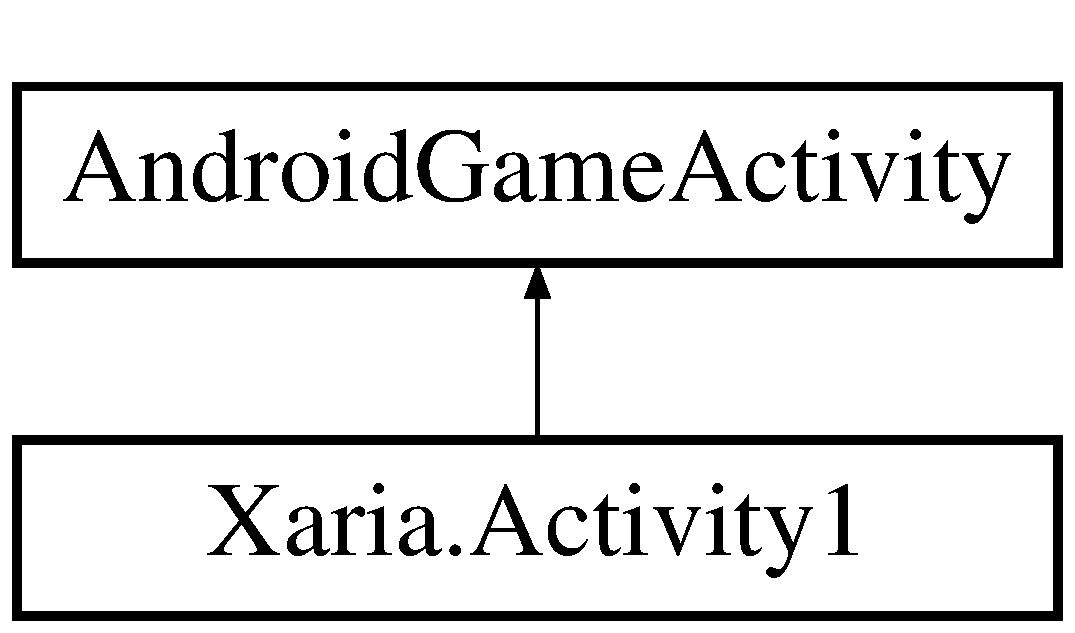
\includegraphics[height=2.000000cm]{classXaria_1_1Activity1}
\end{center}
\end{figure}
\subsection*{Public Member Functions}
\begin{DoxyCompactItemize}
\item 
void \hyperlink{classXaria_1_1Activity1_aadf94688926beaaf66d1000b73662a43}{On\+Accuracy\+Changed} (Sensor sensor, Sensor\+Status accuracy)
\begin{DoxyCompactList}\small\item\em Called when the accuracy of a sensor has changed. \end{DoxyCompactList}\item 
void \hyperlink{classXaria_1_1Activity1_a9a7df9c23656ef7839a8fddd1e14dc49}{On\+Sensor\+Changed} (Sensor\+Event e)
\begin{DoxyCompactList}\small\item\em Called when sensor values have changed. \end{DoxyCompactList}\item 
override bool \hyperlink{classXaria_1_1Activity1_ab27a73ce9dd28a79774b7c10e3630235}{On\+Key\+Up} (\mbox{[}Generated\+Enum\mbox{]} Keycode key\+Code, Key\+Event e)
\begin{DoxyCompactList}\small\item\em Called when a key was released and not handled by any of the views inside of the activity. \end{DoxyCompactList}\end{DoxyCompactItemize}
\subsection*{Static Public Attributes}
\begin{DoxyCompactItemize}
\item 
static Sensor\+Manager \hyperlink{classXaria_1_1Activity1_a24e5f33379e7c617726f819305e211a1}{sensor\+Manager}
\begin{DoxyCompactList}\small\item\em The sensor manager \end{DoxyCompactList}\item 
static float \mbox{[}$\,$\mbox{]} \hyperlink{classXaria_1_1Activity1_a27724ecd7f40103c5f2e1175d4138283}{accel\+Values} = new float\mbox{[}3\mbox{]}
\begin{DoxyCompactList}\small\item\em The accel values \end{DoxyCompactList}\item 
static float \mbox{[}$\,$\mbox{]} \hyperlink{classXaria_1_1Activity1_a258919f676bc970cf2b0742591932ba9}{magneto\+Values} = new float\mbox{[}3\mbox{]}
\begin{DoxyCompactList}\small\item\em The magneto values \end{DoxyCompactList}\end{DoxyCompactItemize}
\subsection*{Protected Member Functions}
\begin{DoxyCompactItemize}
\item 
override void \hyperlink{classXaria_1_1Activity1_a1b2c637e080b9032389a43705d193581}{On\+Create} (Bundle bundle)
\begin{DoxyCompactList}\small\item\em Android activity creation event \end{DoxyCompactList}\end{DoxyCompactItemize}
\subsection*{Private Attributes}
\begin{DoxyCompactItemize}
\item 
Sensor \hyperlink{classXaria_1_1Activity1_a60c77f521c1a61fe00fad362d9cae9ea}{accelerometer}
\begin{DoxyCompactList}\small\item\em The accelerometer \end{DoxyCompactList}\item 
Sensor \hyperlink{classXaria_1_1Activity1_a7fd08945593fa05793e41e4e52818636}{magnetometer}
\begin{DoxyCompactList}\small\item\em The magnetometer \end{DoxyCompactList}\end{DoxyCompactItemize}


\subsection{Detailed Description}
The android activity 

\begin{DoxySeeAlso}{See also}
Android.\+Hardware.\+I\+Sensor\+Event\+Listener, Microsoft.\+Xna.\+Framework.\+Android\+Game\+Activity


\end{DoxySeeAlso}


\subsection{Member Function Documentation}
\mbox{\Hypertarget{classXaria_1_1Activity1_aadf94688926beaaf66d1000b73662a43}\label{classXaria_1_1Activity1_aadf94688926beaaf66d1000b73662a43}} 
\index{Xaria\+::\+Activity1@{Xaria\+::\+Activity1}!On\+Accuracy\+Changed@{On\+Accuracy\+Changed}}
\index{On\+Accuracy\+Changed@{On\+Accuracy\+Changed}!Xaria\+::\+Activity1@{Xaria\+::\+Activity1}}
\subsubsection{\texorpdfstring{On\+Accuracy\+Changed()}{OnAccuracyChanged()}}
{\footnotesize\ttfamily void Xaria.\+Activity1.\+On\+Accuracy\+Changed (\begin{DoxyParamCaption}\item[{Sensor}]{sensor,  }\item[{Sensor\+Status}]{accuracy }\end{DoxyParamCaption})\hspace{0.3cm}{\ttfamily [inline]}}



Called when the accuracy of a sensor has changed. 


\begin{DoxyParams}{Parameters}
{\em sensor} & To be added.\\
\hline
{\em accuracy} & The new accuracy of this sensor\\
\hline
\end{DoxyParams}


Called when the accuracy of a sensor has changed. 

See {\ttfamily T\+:\+Android.\+Hardware.\+Sensor\+Manager} for details.

$<$format type=\char`\"{}text/html\char`\"{}$>$ \href{http://developer.android.com/reference/android/hardware/SensorEventListener.html#onAccuracyChanged(android.hardware.Sensor, int)}{\tt \mbox{[}Android Documentation\mbox{]}} $<$/format$>$ 

$<$since version=\char`\"{}\+Added in A\+P\+I level 3\char`\"{}$>$ \mbox{\Hypertarget{classXaria_1_1Activity1_a1b2c637e080b9032389a43705d193581}\label{classXaria_1_1Activity1_a1b2c637e080b9032389a43705d193581}} 
\index{Xaria\+::\+Activity1@{Xaria\+::\+Activity1}!On\+Create@{On\+Create}}
\index{On\+Create@{On\+Create}!Xaria\+::\+Activity1@{Xaria\+::\+Activity1}}
\subsubsection{\texorpdfstring{On\+Create()}{OnCreate()}}
{\footnotesize\ttfamily override void Xaria.\+Activity1.\+On\+Create (\begin{DoxyParamCaption}\item[{Bundle}]{bundle }\end{DoxyParamCaption})\hspace{0.3cm}{\ttfamily [inline]}, {\ttfamily [protected]}}



Android activity creation event 


\begin{DoxyParams}{Parameters}
{\em bundle} & The bundle.\\
\hline
\end{DoxyParams}
\mbox{\Hypertarget{classXaria_1_1Activity1_ab27a73ce9dd28a79774b7c10e3630235}\label{classXaria_1_1Activity1_ab27a73ce9dd28a79774b7c10e3630235}} 
\index{Xaria\+::\+Activity1@{Xaria\+::\+Activity1}!On\+Key\+Up@{On\+Key\+Up}}
\index{On\+Key\+Up@{On\+Key\+Up}!Xaria\+::\+Activity1@{Xaria\+::\+Activity1}}
\subsubsection{\texorpdfstring{On\+Key\+Up()}{OnKeyUp()}}
{\footnotesize\ttfamily override bool Xaria.\+Activity1.\+On\+Key\+Up (\begin{DoxyParamCaption}\item[{\mbox{[}\+Generated\+Enum\mbox{]} Keycode}]{key\+Code,  }\item[{Key\+Event}]{e }\end{DoxyParamCaption})\hspace{0.3cm}{\ttfamily [inline]}}



Called when a key was released and not handled by any of the views inside of the activity. 


\begin{DoxyParams}{Parameters}
{\em key\+Code} & The value in event.\+get\+Key\+Code().\\
\hline
{\em e} & Description of the key event.\\
\hline
\end{DoxyParams}
\begin{DoxyReturn}{Returns}
To be added. 
\end{DoxyReturn}


Called when a key was released and not handled by any of the views inside of the activity. So, for example, key presses while the cursor is inside a Text\+View will not trigger the event (unless it is a navigation to another object) because Text\+View handles its own key presses. 

The default implementation handles K\+E\+Y\+C\+O\+D\+E\+\_\+\+B\+A\+CK to stop the activity and go back.

$<$format type=\char`\"{}text/html\char`\"{}$>$ \href{http://developer.android.com/reference/android/app/Activity.html#onKeyUp(int, android.view.KeyEvent)}{\tt \mbox{[}Android Documentation\mbox{]}} $<$/format$>$ 

$<$since version=\char`\"{}\+Added in A\+P\+I level 1\char`\"{}$>$ $<$altmember cref=\char`\"{}\+M\+:\+Android.\+App.\+Activity.\+On\+Key\+Down(\+Android.\+Views.\+Keycode, Android.\+Views.\+Key\+Event)\char`\"{}$>$ $<$altmember cref=\char`\"{}\+T\+:\+Android.\+Views.\+Key\+Event\char`\"{}$>$ \mbox{\Hypertarget{classXaria_1_1Activity1_a9a7df9c23656ef7839a8fddd1e14dc49}\label{classXaria_1_1Activity1_a9a7df9c23656ef7839a8fddd1e14dc49}} 
\index{Xaria\+::\+Activity1@{Xaria\+::\+Activity1}!On\+Sensor\+Changed@{On\+Sensor\+Changed}}
\index{On\+Sensor\+Changed@{On\+Sensor\+Changed}!Xaria\+::\+Activity1@{Xaria\+::\+Activity1}}
\subsubsection{\texorpdfstring{On\+Sensor\+Changed()}{OnSensorChanged()}}
{\footnotesize\ttfamily void Xaria.\+Activity1.\+On\+Sensor\+Changed (\begin{DoxyParamCaption}\item[{Sensor\+Event}]{e }\end{DoxyParamCaption})\hspace{0.3cm}{\ttfamily [inline]}}



Called when sensor values have changed. 


\begin{DoxyParams}{Parameters}
{\em e} & the {\ttfamily T\+:\+Android.\+Hardware.\+Sensor\+Event}.\\
\hline
\end{DoxyParams}


Called when sensor values have changed. 

See {\ttfamily T\+:\+Android.\+Hardware.\+Sensor\+Manager} for details on possible sensor types. 

See also {\ttfamily T\+:\+Android.\+Hardware.\+Sensor\+Event}. 

$<$format type=\char`\"{}text/html\char`\"{}$>$ {\bfseries N\+O\+TE\+:} $<$/format$>$ The application doesn\textquotesingle{}t own the {\ttfamily T\+:\+Android.\+Hardware.\+Sensor\+Event} object passed as a parameter and therefore cannot hold on to it. The object may be part of an internal pool and may be reused by the framework.

$<$format type=\char`\"{}text/html\char`\"{}$>$ \href{http://developer.android.com/reference/android/hardware/SensorEventListener.html#onSensorChanged(android.hardware.SensorEvent)}{\tt \mbox{[}Android Documentation\mbox{]}} $<$/format$>$ 

$<$since version=\char`\"{}\+Added in A\+P\+I level 3\char`\"{}$>$ 

\subsection{Member Data Documentation}
\mbox{\Hypertarget{classXaria_1_1Activity1_a60c77f521c1a61fe00fad362d9cae9ea}\label{classXaria_1_1Activity1_a60c77f521c1a61fe00fad362d9cae9ea}} 
\index{Xaria\+::\+Activity1@{Xaria\+::\+Activity1}!accelerometer@{accelerometer}}
\index{accelerometer@{accelerometer}!Xaria\+::\+Activity1@{Xaria\+::\+Activity1}}
\subsubsection{\texorpdfstring{accelerometer}{accelerometer}}
{\footnotesize\ttfamily Sensor Xaria.\+Activity1.\+accelerometer\hspace{0.3cm}{\ttfamily [private]}}



The accelerometer 

\mbox{\Hypertarget{classXaria_1_1Activity1_a27724ecd7f40103c5f2e1175d4138283}\label{classXaria_1_1Activity1_a27724ecd7f40103c5f2e1175d4138283}} 
\index{Xaria\+::\+Activity1@{Xaria\+::\+Activity1}!accel\+Values@{accel\+Values}}
\index{accel\+Values@{accel\+Values}!Xaria\+::\+Activity1@{Xaria\+::\+Activity1}}
\subsubsection{\texorpdfstring{accel\+Values}{accelValues}}
{\footnotesize\ttfamily float \mbox{[}$\,$\mbox{]} Xaria.\+Activity1.\+accel\+Values = new float\mbox{[}3\mbox{]}\hspace{0.3cm}{\ttfamily [static]}}



The accel values 

\mbox{\Hypertarget{classXaria_1_1Activity1_a7fd08945593fa05793e41e4e52818636}\label{classXaria_1_1Activity1_a7fd08945593fa05793e41e4e52818636}} 
\index{Xaria\+::\+Activity1@{Xaria\+::\+Activity1}!magnetometer@{magnetometer}}
\index{magnetometer@{magnetometer}!Xaria\+::\+Activity1@{Xaria\+::\+Activity1}}
\subsubsection{\texorpdfstring{magnetometer}{magnetometer}}
{\footnotesize\ttfamily Sensor Xaria.\+Activity1.\+magnetometer\hspace{0.3cm}{\ttfamily [private]}}



The magnetometer 

\mbox{\Hypertarget{classXaria_1_1Activity1_a258919f676bc970cf2b0742591932ba9}\label{classXaria_1_1Activity1_a258919f676bc970cf2b0742591932ba9}} 
\index{Xaria\+::\+Activity1@{Xaria\+::\+Activity1}!magneto\+Values@{magneto\+Values}}
\index{magneto\+Values@{magneto\+Values}!Xaria\+::\+Activity1@{Xaria\+::\+Activity1}}
\subsubsection{\texorpdfstring{magneto\+Values}{magnetoValues}}
{\footnotesize\ttfamily float \mbox{[}$\,$\mbox{]} Xaria.\+Activity1.\+magneto\+Values = new float\mbox{[}3\mbox{]}\hspace{0.3cm}{\ttfamily [static]}}



The magneto values 

\mbox{\Hypertarget{classXaria_1_1Activity1_a24e5f33379e7c617726f819305e211a1}\label{classXaria_1_1Activity1_a24e5f33379e7c617726f819305e211a1}} 
\index{Xaria\+::\+Activity1@{Xaria\+::\+Activity1}!sensor\+Manager@{sensor\+Manager}}
\index{sensor\+Manager@{sensor\+Manager}!Xaria\+::\+Activity1@{Xaria\+::\+Activity1}}
\subsubsection{\texorpdfstring{sensor\+Manager}{sensorManager}}
{\footnotesize\ttfamily Sensor\+Manager Xaria.\+Activity1.\+sensor\+Manager\hspace{0.3cm}{\ttfamily [static]}}



The sensor manager 



The documentation for this class was generated from the following file\+:\begin{DoxyCompactItemize}
\item 
Project3/\+Project3/Activity1.\+cs\end{DoxyCompactItemize}

\hypertarget{classXaria_1_1Button}{}\section{Xaria.\+Button Class Reference}
\label{classXaria_1_1Button}\index{Xaria.\+Button@{Xaria.\+Button}}


The button class  


Inheritance diagram for Xaria.\+Button\+:\begin{figure}[H]
\begin{center}
\leavevmode
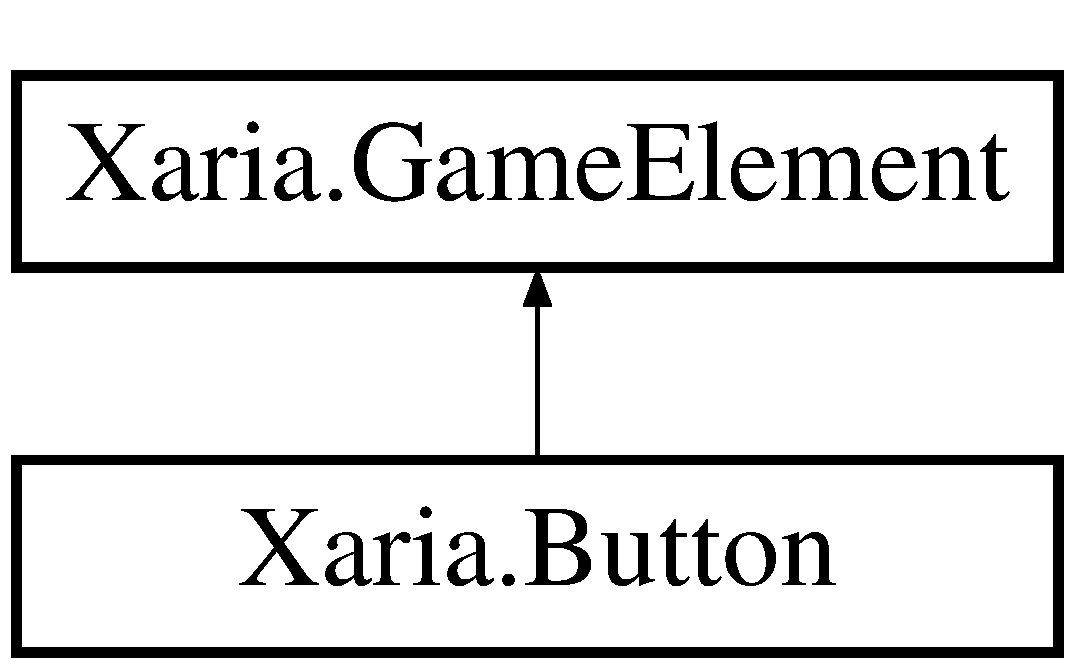
\includegraphics[height=2.000000cm]{classXaria_1_1Button}
\end{center}
\end{figure}
\subsection*{Public Member Functions}
\begin{DoxyCompactItemize}
\item 
\hyperlink{classXaria_1_1Button_adb44a71990a4da16b32e721b30a0d219}{Button} (Texture2D texture, Vector2 position, Action action)
\begin{DoxyCompactList}\small\item\em Initializes a new instance of the \hyperlink{classXaria_1_1Button}{Button} class. \end{DoxyCompactList}\item 
bool \hyperlink{classXaria_1_1Button_aa60b3edf6886916fb025d60db4645ade}{Is\+Clicked} (Touch\+Location input)
\begin{DoxyCompactList}\small\item\em Determines whether the specified input is clicked. \end{DoxyCompactList}\item 
void \hyperlink{classXaria_1_1Button_a774571620215fb6a3b1ae9315023bd41}{Click} ()
\begin{DoxyCompactList}\small\item\em Invokes the click action \end{DoxyCompactList}\end{DoxyCompactItemize}
\subsection*{Private Attributes}
\begin{DoxyCompactItemize}
\item 
Action \hyperlink{classXaria_1_1Button_adbeeb3818c76acb80a43342fc24f1f0f}{click\+Action}
\begin{DoxyCompactList}\small\item\em The click action \end{DoxyCompactList}\end{DoxyCompactItemize}
\subsection*{Additional Inherited Members}


\subsection{Detailed Description}
The button class 

\begin{DoxySeeAlso}{See also}
\hyperlink{classXaria_1_1GameElement}{Xaria.\+Game\+Element}


\end{DoxySeeAlso}


\subsection{Constructor \& Destructor Documentation}
\mbox{\Hypertarget{classXaria_1_1Button_adb44a71990a4da16b32e721b30a0d219}\label{classXaria_1_1Button_adb44a71990a4da16b32e721b30a0d219}} 
\index{Xaria\+::\+Button@{Xaria\+::\+Button}!Button@{Button}}
\index{Button@{Button}!Xaria\+::\+Button@{Xaria\+::\+Button}}
\subsubsection{\texorpdfstring{Button()}{Button()}}
{\footnotesize\ttfamily Xaria.\+Button.\+Button (\begin{DoxyParamCaption}\item[{Texture2D}]{texture,  }\item[{Vector2}]{position,  }\item[{Action}]{action }\end{DoxyParamCaption})\hspace{0.3cm}{\ttfamily [inline]}}



Initializes a new instance of the \hyperlink{classXaria_1_1Button}{Button} class. 


\begin{DoxyParams}{Parameters}
{\em texture} & The texture.\\
\hline
{\em position} & The position.\\
\hline
{\em action} & The action.\\
\hline
\end{DoxyParams}


\subsection{Member Function Documentation}
\mbox{\Hypertarget{classXaria_1_1Button_a774571620215fb6a3b1ae9315023bd41}\label{classXaria_1_1Button_a774571620215fb6a3b1ae9315023bd41}} 
\index{Xaria\+::\+Button@{Xaria\+::\+Button}!Click@{Click}}
\index{Click@{Click}!Xaria\+::\+Button@{Xaria\+::\+Button}}
\subsubsection{\texorpdfstring{Click()}{Click()}}
{\footnotesize\ttfamily void Xaria.\+Button.\+Click (\begin{DoxyParamCaption}{ }\end{DoxyParamCaption})\hspace{0.3cm}{\ttfamily [inline]}}



Invokes the click action 

\mbox{\Hypertarget{classXaria_1_1Button_aa60b3edf6886916fb025d60db4645ade}\label{classXaria_1_1Button_aa60b3edf6886916fb025d60db4645ade}} 
\index{Xaria\+::\+Button@{Xaria\+::\+Button}!Is\+Clicked@{Is\+Clicked}}
\index{Is\+Clicked@{Is\+Clicked}!Xaria\+::\+Button@{Xaria\+::\+Button}}
\subsubsection{\texorpdfstring{Is\+Clicked()}{IsClicked()}}
{\footnotesize\ttfamily bool Xaria.\+Button.\+Is\+Clicked (\begin{DoxyParamCaption}\item[{Touch\+Location}]{input }\end{DoxyParamCaption})\hspace{0.3cm}{\ttfamily [inline]}}



Determines whether the specified input is clicked. 


\begin{DoxyParams}{Parameters}
{\em input} & The input.\\
\hline
\end{DoxyParams}
\begin{DoxyReturn}{Returns}
{\ttfamily true} if the specified input is clicked; otherwise, {\ttfamily false}. 
\end{DoxyReturn}


\subsection{Member Data Documentation}
\mbox{\Hypertarget{classXaria_1_1Button_adbeeb3818c76acb80a43342fc24f1f0f}\label{classXaria_1_1Button_adbeeb3818c76acb80a43342fc24f1f0f}} 
\index{Xaria\+::\+Button@{Xaria\+::\+Button}!click\+Action@{click\+Action}}
\index{click\+Action@{click\+Action}!Xaria\+::\+Button@{Xaria\+::\+Button}}
\subsubsection{\texorpdfstring{click\+Action}{clickAction}}
{\footnotesize\ttfamily Action Xaria.\+Button.\+click\+Action\hspace{0.3cm}{\ttfamily [private]}}



The click action 



The documentation for this class was generated from the following file\+:\begin{DoxyCompactItemize}
\item 
Project3/\+Project3/Button.\+cs\end{DoxyCompactItemize}

\hypertarget{classXaria_1_1Game1}{}\section{Xaria.\+Game1 Class Reference}
\label{classXaria_1_1Game1}\index{Xaria.\+Game1@{Xaria.\+Game1}}


This is the main type for your game.  


Inheritance diagram for Xaria.\+Game1\+:\begin{figure}[H]
\begin{center}
\leavevmode
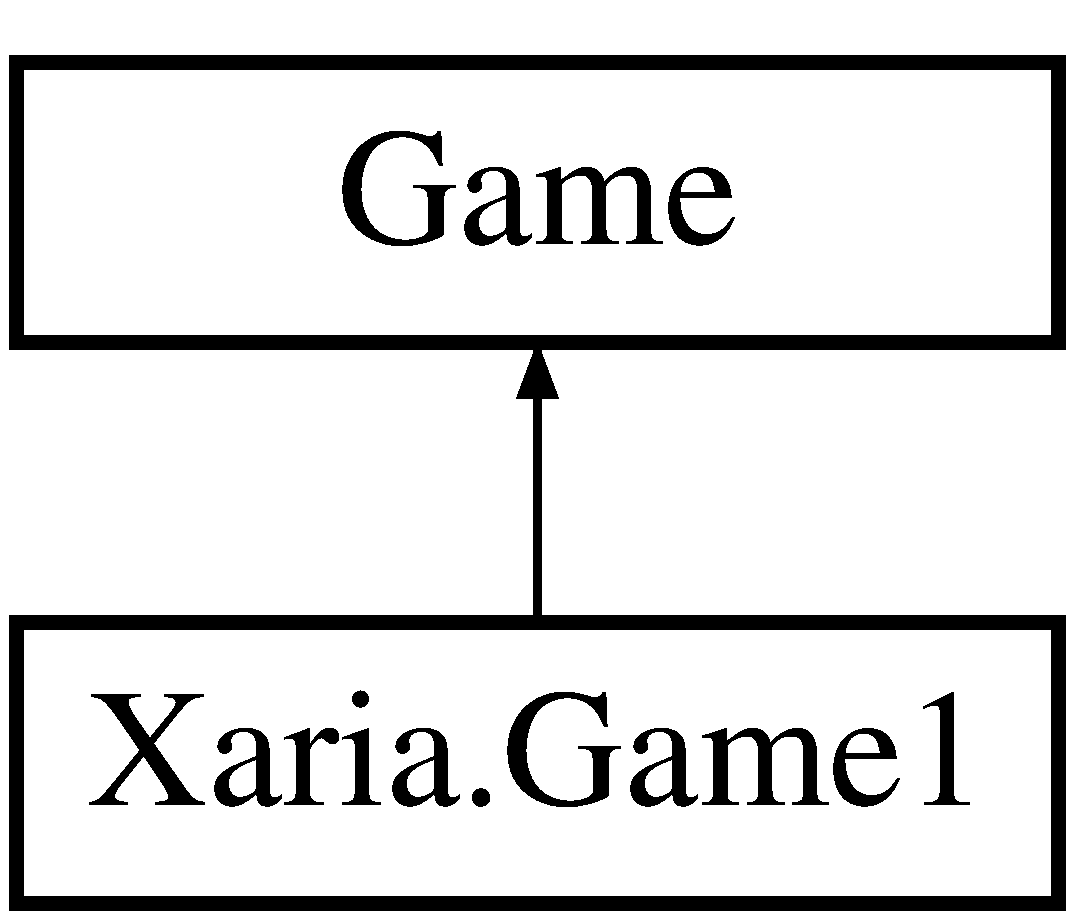
\includegraphics[height=2.000000cm]{classXaria_1_1Game1}
\end{center}
\end{figure}
\subsection*{Public Member Functions}
\begin{DoxyCompactItemize}
\item 
\hyperlink{classXaria_1_1Game1_aa7b8268d52c2f0435734c83f3d76f266}{Game1} ()
\begin{DoxyCompactList}\small\item\em Initializes a new instance of the \hyperlink{classXaria_1_1Game1}{Game1} class. \end{DoxyCompactList}\end{DoxyCompactItemize}
\subsection*{Protected Member Functions}
\begin{DoxyCompactItemize}
\item 
override void \hyperlink{classXaria_1_1Game1_a7510c981afe40f31d24c551b7cc73046}{Initialize} ()
\begin{DoxyCompactList}\small\item\em Allows the game to perform any initialization it needs to before starting to run. This is where it can query for any required services and load any non-\/graphic related content. Calling base.\+Initialize will enumerate through any components and initialize them as well. \end{DoxyCompactList}\item 
override void \hyperlink{classXaria_1_1Game1_a4593eda6c63d3242f6544e2357a08431}{Load\+Content} ()
\begin{DoxyCompactList}\small\item\em Load\+Content will be called once per game and is the place to load all of your content. \end{DoxyCompactList}\item 
override void \hyperlink{classXaria_1_1Game1_a650e782700008533feec6ae84c19536a}{Update} (Game\+Time game\+Time)
\begin{DoxyCompactList}\small\item\em Allows the game to run logic such as updating the world, checking for collisions, gathering input, and playing audio. \end{DoxyCompactList}\item 
override void \hyperlink{classXaria_1_1Game1_a5dce3a85b3eba6685d04d309bcd6e1c0}{Draw} (Game\+Time game\+Time)
\begin{DoxyCompactList}\small\item\em This is called when the game should draw itself. \end{DoxyCompactList}\end{DoxyCompactItemize}
\subsection*{Static Package Attributes}
\begin{DoxyCompactItemize}
\item 
static Vector2 \hyperlink{classXaria_1_1Game1_a898cce284fb6f0610dc80b644b2515e8}{scale}
\begin{DoxyCompactList}\small\item\em The scale for game drawing \end{DoxyCompactList}\item 
static Vector2 \hyperlink{classXaria_1_1Game1_a6ed6553ba5719c56420ea91daf45baac}{screen\+Size}
\begin{DoxyCompactList}\small\item\em The screen size \end{DoxyCompactList}\item 
static Dictionary$<$ string, Texture2D $>$ \hyperlink{classXaria_1_1Game1_a4b450443afb4c333b7c1e4f52beaebb8}{texture\+Dictionary} = new Dictionary$<$string, Texture2D$>$()
\begin{DoxyCompactList}\small\item\em The texture dictionary \end{DoxyCompactList}\item 
static \hyperlink{namespaceXaria_a2c2420c982c39ab01bdb72f1d7d4aac7}{Game\+State} \hyperlink{classXaria_1_1Game1_aba3abde5ccacf8d7e06d7eddf07a32ef}{state} = \hyperlink{namespaceXaria_a2c2420c982c39ab01bdb72f1d7d4aac7aa6122a65eaa676f700ae68d393054a37}{Game\+State.\+Start}
\begin{DoxyCompactList}\small\item\em The state \end{DoxyCompactList}\item 
static Sprite\+Font \hyperlink{classXaria_1_1Game1_a5693ebed547453aca51068c8f941c690}{font}
\begin{DoxyCompactList}\small\item\em The font \end{DoxyCompactList}\item 
static \hyperlink{classXaria_1_1Player}{Player} \hyperlink{classXaria_1_1Game1_a4bd930c3ac170ab2e202b58bb093eb81}{player}
\begin{DoxyCompactList}\small\item\em The player \end{DoxyCompactList}\item 
static \hyperlink{classXaria_1_1Level}{Level} \hyperlink{classXaria_1_1Game1_a0923aa0c8e68d0408afab30eb1817e5e}{level}
\begin{DoxyCompactList}\small\item\em The level \end{DoxyCompactList}\end{DoxyCompactItemize}
\subsection*{Private Attributes}
\begin{DoxyCompactItemize}
\item 
Graphics\+Device\+Manager \hyperlink{classXaria_1_1Game1_a1bbdbcd137d3484aa8c662c8574ac1a3}{graphics}
\begin{DoxyCompactList}\small\item\em The graphics device manager \end{DoxyCompactList}\item 
Sprite\+Batch \hyperlink{classXaria_1_1Game1_a5c9ecabcaf53ac9aa1a8fd1d18a9e585}{sprite\+Batch}
\begin{DoxyCompactList}\small\item\em The sprite batch for drawings \end{DoxyCompactList}\item 
\hyperlink{namespaceXaria_a2c2420c982c39ab01bdb72f1d7d4aac7aa6122a65eaa676f700ae68d393054a37}{Start} \hyperlink{classXaria_1_1Game1_a6707e2f65e76cd15207852d0f502f07c}{start\+Screen}
\begin{DoxyCompactList}\small\item\em The start screen \end{DoxyCompactList}\item 
\hyperlink{namespaceXaria_a2c2420c982c39ab01bdb72f1d7d4aac7a87557f11575c0ad78e4e28abedc13b6e}{End} \hyperlink{classXaria_1_1Game1_a24d32974a54581bfc6931f9dd8b3b107}{end\+Screen}
\begin{DoxyCompactList}\small\item\em The end screen \end{DoxyCompactList}\item 
Background \hyperlink{classXaria_1_1Game1_a78d1a6b1749b5d112ca90524a74728ed}{background}
\begin{DoxyCompactList}\small\item\em The background \end{DoxyCompactList}\end{DoxyCompactItemize}


\subsection{Detailed Description}
This is the main type for your game. 



\subsection{Constructor \& Destructor Documentation}
\mbox{\Hypertarget{classXaria_1_1Game1_aa7b8268d52c2f0435734c83f3d76f266}\label{classXaria_1_1Game1_aa7b8268d52c2f0435734c83f3d76f266}} 
\index{Xaria\+::\+Game1@{Xaria\+::\+Game1}!Game1@{Game1}}
\index{Game1@{Game1}!Xaria\+::\+Game1@{Xaria\+::\+Game1}}
\subsubsection{\texorpdfstring{Game1()}{Game1()}}
{\footnotesize\ttfamily Xaria.\+Game1.\+Game1 (\begin{DoxyParamCaption}{ }\end{DoxyParamCaption})\hspace{0.3cm}{\ttfamily [inline]}}



Initializes a new instance of the \hyperlink{classXaria_1_1Game1}{Game1} class. 



\subsection{Member Function Documentation}
\mbox{\Hypertarget{classXaria_1_1Game1_a5dce3a85b3eba6685d04d309bcd6e1c0}\label{classXaria_1_1Game1_a5dce3a85b3eba6685d04d309bcd6e1c0}} 
\index{Xaria\+::\+Game1@{Xaria\+::\+Game1}!Draw@{Draw}}
\index{Draw@{Draw}!Xaria\+::\+Game1@{Xaria\+::\+Game1}}
\subsubsection{\texorpdfstring{Draw()}{Draw()}}
{\footnotesize\ttfamily override void Xaria.\+Game1.\+Draw (\begin{DoxyParamCaption}\item[{Game\+Time}]{game\+Time }\end{DoxyParamCaption})\hspace{0.3cm}{\ttfamily [inline]}, {\ttfamily [protected]}}



This is called when the game should draw itself. 


\begin{DoxyParams}{Parameters}
{\em game\+Time} & Provides a snapshot of timing values.\\
\hline
\end{DoxyParams}
\mbox{\Hypertarget{classXaria_1_1Game1_a7510c981afe40f31d24c551b7cc73046}\label{classXaria_1_1Game1_a7510c981afe40f31d24c551b7cc73046}} 
\index{Xaria\+::\+Game1@{Xaria\+::\+Game1}!Initialize@{Initialize}}
\index{Initialize@{Initialize}!Xaria\+::\+Game1@{Xaria\+::\+Game1}}
\subsubsection{\texorpdfstring{Initialize()}{Initialize()}}
{\footnotesize\ttfamily override void Xaria.\+Game1.\+Initialize (\begin{DoxyParamCaption}{ }\end{DoxyParamCaption})\hspace{0.3cm}{\ttfamily [inline]}, {\ttfamily [protected]}}



Allows the game to perform any initialization it needs to before starting to run. This is where it can query for any required services and load any non-\/graphic related content. Calling base.\+Initialize will enumerate through any components and initialize them as well. 

\mbox{\Hypertarget{classXaria_1_1Game1_a4593eda6c63d3242f6544e2357a08431}\label{classXaria_1_1Game1_a4593eda6c63d3242f6544e2357a08431}} 
\index{Xaria\+::\+Game1@{Xaria\+::\+Game1}!Load\+Content@{Load\+Content}}
\index{Load\+Content@{Load\+Content}!Xaria\+::\+Game1@{Xaria\+::\+Game1}}
\subsubsection{\texorpdfstring{Load\+Content()}{LoadContent()}}
{\footnotesize\ttfamily override void Xaria.\+Game1.\+Load\+Content (\begin{DoxyParamCaption}{ }\end{DoxyParamCaption})\hspace{0.3cm}{\ttfamily [inline]}, {\ttfamily [protected]}}



Load\+Content will be called once per game and is the place to load all of your content. 

\mbox{\Hypertarget{classXaria_1_1Game1_a650e782700008533feec6ae84c19536a}\label{classXaria_1_1Game1_a650e782700008533feec6ae84c19536a}} 
\index{Xaria\+::\+Game1@{Xaria\+::\+Game1}!Update@{Update}}
\index{Update@{Update}!Xaria\+::\+Game1@{Xaria\+::\+Game1}}
\subsubsection{\texorpdfstring{Update()}{Update()}}
{\footnotesize\ttfamily override void Xaria.\+Game1.\+Update (\begin{DoxyParamCaption}\item[{Game\+Time}]{game\+Time }\end{DoxyParamCaption})\hspace{0.3cm}{\ttfamily [inline]}, {\ttfamily [protected]}}



Allows the game to run logic such as updating the world, checking for collisions, gathering input, and playing audio. 


\begin{DoxyParams}{Parameters}
{\em game\+Time} & Provides a snapshot of timing values.\\
\hline
\end{DoxyParams}


\subsection{Member Data Documentation}
\mbox{\Hypertarget{classXaria_1_1Game1_a78d1a6b1749b5d112ca90524a74728ed}\label{classXaria_1_1Game1_a78d1a6b1749b5d112ca90524a74728ed}} 
\index{Xaria\+::\+Game1@{Xaria\+::\+Game1}!background@{background}}
\index{background@{background}!Xaria\+::\+Game1@{Xaria\+::\+Game1}}
\subsubsection{\texorpdfstring{background}{background}}
{\footnotesize\ttfamily Background Xaria.\+Game1.\+background\hspace{0.3cm}{\ttfamily [private]}}



The background 

\mbox{\Hypertarget{classXaria_1_1Game1_a24d32974a54581bfc6931f9dd8b3b107}\label{classXaria_1_1Game1_a24d32974a54581bfc6931f9dd8b3b107}} 
\index{Xaria\+::\+Game1@{Xaria\+::\+Game1}!end\+Screen@{end\+Screen}}
\index{end\+Screen@{end\+Screen}!Xaria\+::\+Game1@{Xaria\+::\+Game1}}
\subsubsection{\texorpdfstring{end\+Screen}{endScreen}}
{\footnotesize\ttfamily \hyperlink{namespaceXaria_a2c2420c982c39ab01bdb72f1d7d4aac7a87557f11575c0ad78e4e28abedc13b6e}{End} Xaria.\+Game1.\+end\+Screen\hspace{0.3cm}{\ttfamily [private]}}



The end screen 

\mbox{\Hypertarget{classXaria_1_1Game1_a5693ebed547453aca51068c8f941c690}\label{classXaria_1_1Game1_a5693ebed547453aca51068c8f941c690}} 
\index{Xaria\+::\+Game1@{Xaria\+::\+Game1}!font@{font}}
\index{font@{font}!Xaria\+::\+Game1@{Xaria\+::\+Game1}}
\subsubsection{\texorpdfstring{font}{font}}
{\footnotesize\ttfamily Sprite\+Font Xaria.\+Game1.\+font\hspace{0.3cm}{\ttfamily [static]}, {\ttfamily [package]}}



The font 

\mbox{\Hypertarget{classXaria_1_1Game1_a1bbdbcd137d3484aa8c662c8574ac1a3}\label{classXaria_1_1Game1_a1bbdbcd137d3484aa8c662c8574ac1a3}} 
\index{Xaria\+::\+Game1@{Xaria\+::\+Game1}!graphics@{graphics}}
\index{graphics@{graphics}!Xaria\+::\+Game1@{Xaria\+::\+Game1}}
\subsubsection{\texorpdfstring{graphics}{graphics}}
{\footnotesize\ttfamily Graphics\+Device\+Manager Xaria.\+Game1.\+graphics\hspace{0.3cm}{\ttfamily [private]}}



The graphics device manager 

\mbox{\Hypertarget{classXaria_1_1Game1_a0923aa0c8e68d0408afab30eb1817e5e}\label{classXaria_1_1Game1_a0923aa0c8e68d0408afab30eb1817e5e}} 
\index{Xaria\+::\+Game1@{Xaria\+::\+Game1}!level@{level}}
\index{level@{level}!Xaria\+::\+Game1@{Xaria\+::\+Game1}}
\subsubsection{\texorpdfstring{level}{level}}
{\footnotesize\ttfamily \hyperlink{classXaria_1_1Level}{Level} Xaria.\+Game1.\+level\hspace{0.3cm}{\ttfamily [static]}, {\ttfamily [package]}}



The level 

\mbox{\Hypertarget{classXaria_1_1Game1_a4bd930c3ac170ab2e202b58bb093eb81}\label{classXaria_1_1Game1_a4bd930c3ac170ab2e202b58bb093eb81}} 
\index{Xaria\+::\+Game1@{Xaria\+::\+Game1}!player@{player}}
\index{player@{player}!Xaria\+::\+Game1@{Xaria\+::\+Game1}}
\subsubsection{\texorpdfstring{player}{player}}
{\footnotesize\ttfamily \hyperlink{classXaria_1_1Player}{Player} Xaria.\+Game1.\+player\hspace{0.3cm}{\ttfamily [static]}, {\ttfamily [package]}}



The player 

\mbox{\Hypertarget{classXaria_1_1Game1_a898cce284fb6f0610dc80b644b2515e8}\label{classXaria_1_1Game1_a898cce284fb6f0610dc80b644b2515e8}} 
\index{Xaria\+::\+Game1@{Xaria\+::\+Game1}!scale@{scale}}
\index{scale@{scale}!Xaria\+::\+Game1@{Xaria\+::\+Game1}}
\subsubsection{\texorpdfstring{scale}{scale}}
{\footnotesize\ttfamily Vector2 Xaria.\+Game1.\+scale\hspace{0.3cm}{\ttfamily [static]}, {\ttfamily [package]}}



The scale for game drawing 

\mbox{\Hypertarget{classXaria_1_1Game1_a6ed6553ba5719c56420ea91daf45baac}\label{classXaria_1_1Game1_a6ed6553ba5719c56420ea91daf45baac}} 
\index{Xaria\+::\+Game1@{Xaria\+::\+Game1}!screen\+Size@{screen\+Size}}
\index{screen\+Size@{screen\+Size}!Xaria\+::\+Game1@{Xaria\+::\+Game1}}
\subsubsection{\texorpdfstring{screen\+Size}{screenSize}}
{\footnotesize\ttfamily Vector2 Xaria.\+Game1.\+screen\+Size\hspace{0.3cm}{\ttfamily [static]}, {\ttfamily [package]}}



The screen size 

\mbox{\Hypertarget{classXaria_1_1Game1_a5c9ecabcaf53ac9aa1a8fd1d18a9e585}\label{classXaria_1_1Game1_a5c9ecabcaf53ac9aa1a8fd1d18a9e585}} 
\index{Xaria\+::\+Game1@{Xaria\+::\+Game1}!sprite\+Batch@{sprite\+Batch}}
\index{sprite\+Batch@{sprite\+Batch}!Xaria\+::\+Game1@{Xaria\+::\+Game1}}
\subsubsection{\texorpdfstring{sprite\+Batch}{spriteBatch}}
{\footnotesize\ttfamily Sprite\+Batch Xaria.\+Game1.\+sprite\+Batch\hspace{0.3cm}{\ttfamily [private]}}



The sprite batch for drawings 

\mbox{\Hypertarget{classXaria_1_1Game1_a6707e2f65e76cd15207852d0f502f07c}\label{classXaria_1_1Game1_a6707e2f65e76cd15207852d0f502f07c}} 
\index{Xaria\+::\+Game1@{Xaria\+::\+Game1}!start\+Screen@{start\+Screen}}
\index{start\+Screen@{start\+Screen}!Xaria\+::\+Game1@{Xaria\+::\+Game1}}
\subsubsection{\texorpdfstring{start\+Screen}{startScreen}}
{\footnotesize\ttfamily \hyperlink{namespaceXaria_a2c2420c982c39ab01bdb72f1d7d4aac7aa6122a65eaa676f700ae68d393054a37}{Start} Xaria.\+Game1.\+start\+Screen\hspace{0.3cm}{\ttfamily [private]}}



The start screen 

\mbox{\Hypertarget{classXaria_1_1Game1_aba3abde5ccacf8d7e06d7eddf07a32ef}\label{classXaria_1_1Game1_aba3abde5ccacf8d7e06d7eddf07a32ef}} 
\index{Xaria\+::\+Game1@{Xaria\+::\+Game1}!state@{state}}
\index{state@{state}!Xaria\+::\+Game1@{Xaria\+::\+Game1}}
\subsubsection{\texorpdfstring{state}{state}}
{\footnotesize\ttfamily \hyperlink{namespaceXaria_a2c2420c982c39ab01bdb72f1d7d4aac7}{Game\+State} Xaria.\+Game1.\+state = \hyperlink{namespaceXaria_a2c2420c982c39ab01bdb72f1d7d4aac7aa6122a65eaa676f700ae68d393054a37}{Game\+State.\+Start}\hspace{0.3cm}{\ttfamily [static]}, {\ttfamily [package]}}



The state 

\mbox{\Hypertarget{classXaria_1_1Game1_a4b450443afb4c333b7c1e4f52beaebb8}\label{classXaria_1_1Game1_a4b450443afb4c333b7c1e4f52beaebb8}} 
\index{Xaria\+::\+Game1@{Xaria\+::\+Game1}!texture\+Dictionary@{texture\+Dictionary}}
\index{texture\+Dictionary@{texture\+Dictionary}!Xaria\+::\+Game1@{Xaria\+::\+Game1}}
\subsubsection{\texorpdfstring{texture\+Dictionary}{textureDictionary}}
{\footnotesize\ttfamily Dictionary$<$string, Texture2D$>$ Xaria.\+Game1.\+texture\+Dictionary = new Dictionary$<$string, Texture2D$>$()\hspace{0.3cm}{\ttfamily [static]}, {\ttfamily [package]}}



The texture dictionary 



The documentation for this class was generated from the following file\+:\begin{DoxyCompactItemize}
\item 
Project3/\+Project3/\hyperlink{Game1_8cs}{Game1.\+cs}\end{DoxyCompactItemize}

\hypertarget{classXaria_1_1GameElement}{}\section{Xaria.\+Game\+Element Class Reference}
\label{classXaria_1_1GameElement}\index{Xaria.\+Game\+Element@{Xaria.\+Game\+Element}}


Basic element that stores texture, position, and draw info.  


Inheritance diagram for Xaria.\+Game\+Element\+:\begin{figure}[H]
\begin{center}
\leavevmode
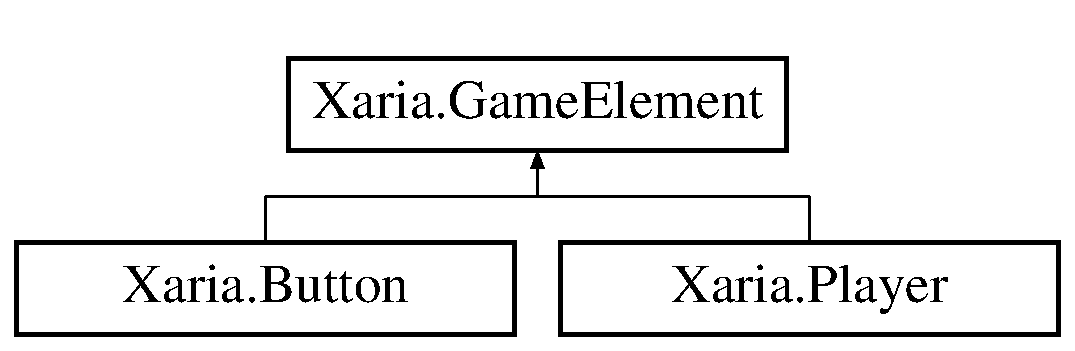
\includegraphics[height=3.218391cm]{classXaria_1_1GameElement}
\end{center}
\end{figure}
\subsection*{Public Member Functions}
\begin{DoxyCompactItemize}
\item 
void \hyperlink{classXaria_1_1GameElement_a7f93dc93e970e72a5540924e06d28c92}{Draw} (ref Sprite\+Batch sprite\+Batch, Color color)
\begin{DoxyCompactList}\small\item\em Draws the specified sprite batch. \end{DoxyCompactList}\item 
virtual void \hyperlink{classXaria_1_1GameElement_a812e0ffbe54519a3fb14a49115bf43d9}{Draw} (ref Sprite\+Batch sprite\+Batch)
\begin{DoxyCompactList}\small\item\em Draws the specified sprite batch. \end{DoxyCompactList}\item 
Rectangle \hyperlink{classXaria_1_1GameElement_a2b050e61aea8232eba3e820b14c98656}{Bounds} ()
\begin{DoxyCompactList}\small\item\em Gets the element\textquotesingle{}s bounds \end{DoxyCompactList}\end{DoxyCompactItemize}
\subsection*{Properties}
\begin{DoxyCompactItemize}
\item 
Texture2D \hyperlink{classXaria_1_1GameElement_ae5816c3fd6f76aa7af85b1cc9c8a5cf8}{Texture}\hspace{0.3cm}{\ttfamily  \mbox{[}get, set\mbox{]}}
\begin{DoxyCompactList}\small\item\em Gets the texture. \end{DoxyCompactList}\end{DoxyCompactItemize}


\subsection{Detailed Description}
Basic element that stores texture, position, and draw info. 



\subsection{Member Function Documentation}
\mbox{\Hypertarget{classXaria_1_1GameElement_a2b050e61aea8232eba3e820b14c98656}\label{classXaria_1_1GameElement_a2b050e61aea8232eba3e820b14c98656}} 
\index{Xaria\+::\+Game\+Element@{Xaria\+::\+Game\+Element}!Bounds@{Bounds}}
\index{Bounds@{Bounds}!Xaria\+::\+Game\+Element@{Xaria\+::\+Game\+Element}}
\subsubsection{\texorpdfstring{Bounds()}{Bounds()}}
{\footnotesize\ttfamily Rectangle Xaria.\+Game\+Element.\+Bounds (\begin{DoxyParamCaption}{ }\end{DoxyParamCaption})\hspace{0.3cm}{\ttfamily [inline]}}



Gets the element\textquotesingle{}s bounds 

\begin{DoxyReturn}{Returns}

\end{DoxyReturn}
\mbox{\Hypertarget{classXaria_1_1GameElement_a7f93dc93e970e72a5540924e06d28c92}\label{classXaria_1_1GameElement_a7f93dc93e970e72a5540924e06d28c92}} 
\index{Xaria\+::\+Game\+Element@{Xaria\+::\+Game\+Element}!Draw@{Draw}}
\index{Draw@{Draw}!Xaria\+::\+Game\+Element@{Xaria\+::\+Game\+Element}}
\subsubsection{\texorpdfstring{Draw()}{Draw()}\hspace{0.1cm}{\footnotesize\ttfamily [1/2]}}
{\footnotesize\ttfamily void Xaria.\+Game\+Element.\+Draw (\begin{DoxyParamCaption}\item[{ref Sprite\+Batch}]{sprite\+Batch,  }\item[{Color}]{color }\end{DoxyParamCaption})\hspace{0.3cm}{\ttfamily [inline]}}



Draws the specified sprite batch. 


\begin{DoxyParams}{Parameters}
{\em sprite\+Batch} & The sprite batch.\\
\hline
{\em color} & The color.\\
\hline
\end{DoxyParams}
\mbox{\Hypertarget{classXaria_1_1GameElement_a812e0ffbe54519a3fb14a49115bf43d9}\label{classXaria_1_1GameElement_a812e0ffbe54519a3fb14a49115bf43d9}} 
\index{Xaria\+::\+Game\+Element@{Xaria\+::\+Game\+Element}!Draw@{Draw}}
\index{Draw@{Draw}!Xaria\+::\+Game\+Element@{Xaria\+::\+Game\+Element}}
\subsubsection{\texorpdfstring{Draw()}{Draw()}\hspace{0.1cm}{\footnotesize\ttfamily [2/2]}}
{\footnotesize\ttfamily virtual void Xaria.\+Game\+Element.\+Draw (\begin{DoxyParamCaption}\item[{ref Sprite\+Batch}]{sprite\+Batch }\end{DoxyParamCaption})\hspace{0.3cm}{\ttfamily [inline]}, {\ttfamily [virtual]}}



Draws the specified sprite batch. 


\begin{DoxyParams}{Parameters}
{\em sprite\+Batch} & The sprite batch.\\
\hline
\end{DoxyParams}


Reimplemented in \hyperlink{classXaria_1_1Player_a25ddea2b9d8679ab6aa649fda6ce1f22}{Xaria.\+Player}, \hyperlink{classXaria_1_1Enemy_a0f857a720f4a5ecc037887c846c55afc}{Xaria.\+Enemy}, and \hyperlink{classXaria_1_1Drops_1_1Drop_a2cd5c3912ae653526a7cc25aefa691b0}{Xaria.\+Drops.\+Drop}.



\subsection{Property Documentation}
\mbox{\Hypertarget{classXaria_1_1GameElement_ae5816c3fd6f76aa7af85b1cc9c8a5cf8}\label{classXaria_1_1GameElement_ae5816c3fd6f76aa7af85b1cc9c8a5cf8}} 
\index{Xaria\+::\+Game\+Element@{Xaria\+::\+Game\+Element}!Texture@{Texture}}
\index{Texture@{Texture}!Xaria\+::\+Game\+Element@{Xaria\+::\+Game\+Element}}
\subsubsection{\texorpdfstring{Texture}{Texture}}
{\footnotesize\ttfamily Texture2D Xaria.\+Game\+Element.\+Texture\hspace{0.3cm}{\ttfamily [get]}, {\ttfamily [set]}, {\ttfamily [protected]}}



Gets the texture. 

The texture. 

The documentation for this class was generated from the following file\+:\begin{DoxyCompactItemize}
\item 
Project3/\+Project3/Game\+Element.\+cs\end{DoxyCompactItemize}

\hypertarget{classXaria_1_1Level}{}\section{Xaria.\+Level Class Reference}
\label{classXaria_1_1Level}\index{Xaria.\+Level@{Xaria.\+Level}}


The \hyperlink{classXaria_1_1Level}{Level} class  


\subsection*{Public Member Functions}
\begin{DoxyCompactItemize}
\item 
\hyperlink{classXaria_1_1Level_abbe8f5dc4eb2b1ea9bb259a4e1440838}{Level} (int difficulty)
\begin{DoxyCompactList}\small\item\em Initializes a new instance of the \hyperlink{classXaria_1_1Level}{Level} class. \end{DoxyCompactList}\end{DoxyCompactItemize}
\subsection*{Public Attributes}
\begin{DoxyCompactItemize}
\item 
const int \hyperlink{classXaria_1_1Level_a7ff38927b2a440eca51807fcc4f53109}{B\+O\+S\+S\+\_\+\+L\+E\+V\+EL} = 4
\begin{DoxyCompactList}\small\item\em The boss level \end{DoxyCompactList}\item 
const int \hyperlink{classXaria_1_1Level_aeefce3beb83d2578ed9f63c59c0a7e9d}{F\+I\+N\+A\+L\+\_\+\+L\+E\+V\+EL} = 16
\begin{DoxyCompactList}\small\item\em The final level \end{DoxyCompactList}\item 
const int \hyperlink{classXaria_1_1Level_afd8806018ddf8b47dbec8a495ed8e3b4}{E\+N\+E\+M\+I\+E\+S\+\_\+\+P\+E\+R\+\_\+\+R\+OW} = 7
\begin{DoxyCompactList}\small\item\em The enemies per row \end{DoxyCompactList}\end{DoxyCompactItemize}
\subsection*{Static Public Attributes}
\begin{DoxyCompactItemize}
\item 
static Random \hyperlink{classXaria_1_1Level_a9782c177ac48834cf40de7ab5a17469f}{random} = new Random()
\begin{DoxyCompactList}\small\item\em A random class for determining enemy shooting \end{DoxyCompactList}\end{DoxyCompactItemize}
\subsection*{Properties}
\begin{DoxyCompactItemize}
\item 
int \hyperlink{classXaria_1_1Level_a088431ceff97978eb6b0c9aae95ccfd2}{Difficulty}\hspace{0.3cm}{\ttfamily  \mbox{[}get, private set\mbox{]}}
\begin{DoxyCompactList}\small\item\em Gets the difficulty. \end{DoxyCompactList}\end{DoxyCompactItemize}
\subsection*{Private Member Functions}
\begin{DoxyCompactItemize}
\item 
void \hyperlink{classXaria_1_1Level_a22bccc0212af3ebce89ad36a735cf2f1}{Generate\+Level} (int difficulty)
\begin{DoxyCompactList}\small\item\em \+: Either the game has just started, or a level was just beaten. Difficulty level is needed. \+: The current level the player needs to go through is generated \+: None. \end{DoxyCompactList}\item 
List$<$ \hyperlink{classXaria_1_1Enemy_af736652ccf0a3aabacb41bd1afd41234}{Enemy.\+Type} $>$ \hyperlink{classXaria_1_1Level_ae564a661679ef491ffc9ec1406a34d51}{Get\+Enemy\+Types} (List$<$ \hyperlink{classXaria_1_1Enemy_af736652ccf0a3aabacb41bd1afd41234}{Enemy.\+Type} $>$ prev\+Level=null, int difficulty=1)
\begin{DoxyCompactList}\small\item\em \+: Requires level difficulty. A new level is needed to be generated. \+: The previous level\textquotesingle{}s row types for the enemy rows is found \+: enemy list for the current level \end{DoxyCompactList}\item 
void \hyperlink{classXaria_1_1Level_a29b52773008e6b0091a896718d4004b0}{Add\+Boss} (\hyperlink{classXaria_1_1Enemies_1_1Boss_ae95ffc3618433440acbfd7aab7671b02}{Boss.\+Type} boss\+Type)
\begin{DoxyCompactList}\small\item\em \+: \hyperlink{classXaria_1_1Level}{Level} 3, 7, 11, or 15 has been completed. A boss is needed for the next level and is generated. \+: Boss is generated \+: None \end{DoxyCompactList}\item 
void \hyperlink{classXaria_1_1Level_a90464cee28b51fe396f2990c15af90f3}{Add\+Row\+Of\+Enemy} (\hyperlink{classXaria_1_1Enemy_af736652ccf0a3aabacb41bd1afd41234}{Enemy.\+Type} enemy\+Type)
\begin{DoxyCompactList}\small\item\em \+: A row of enemies is needed for the next level \+: A level of enemies (basic, intermediate, or advanced) is added to the enemy list \+: None. \end{DoxyCompactList}\item 
void \hyperlink{classXaria_1_1Level_a066f8459e44939f3d2851427dfc3423e}{Update\+Drops} ()
\begin{DoxyCompactList}\small\item\em \+: An enemy has died and powerup drop for the player has been created \+: powerup drop is moved downward until it is off the screen or the player\textquotesingle{}s hitbox intersects the drops hitbox \+: None \end{DoxyCompactList}\item 
void \hyperlink{classXaria_1_1Level_a46a7b08381a882d95321d41f0ab7537f}{Update\+Enemies} (Game\+Time game\+Time)
\begin{DoxyCompactList}\small\item\em \+: The list of enemies has been created. \+: All enemy sprites are updated. This means if their health is below 0, they are removed from the list and the game. Calls Update\+Movement and Shoot on all enemies. \+: None \end{DoxyCompactList}\item 
void \hyperlink{classXaria_1_1Level_a9c32c2aeebc7fefe181b142fe03cae78}{Update\+Enemy\+Projectiles} ()
\begin{DoxyCompactList}\small\item\em \+: An enemy has shot a projectile (decided by R\+NG) \+: All enemy projectiles are moved downward.\+If it intersects the player, the player loses health. \+: None \end{DoxyCompactList}\item 
void \hyperlink{classXaria_1_1Level_ab1b45e8eacae455500518158aceadeba}{Next\+Level} ()
\begin{DoxyCompactList}\small\item\em Goes to the next level. \+: An enemy has shot a projectile (decided by R\+NG) \+: All enemy projectiles are moved downward.\+If it intersects the player, the player loses health. \+: None \end{DoxyCompactList}\item 
void \hyperlink{classXaria_1_1Level_aca4ebca18f725704744d9c51073a44a5}{Game\+Over} ()
\begin{DoxyCompactList}\small\item\em \+: \hyperlink{classXaria_1_1Player}{Player} has beaten the final level (level 16) or has lost all of their lives \+: Game\+State is changed to End \+: None \end{DoxyCompactList}\end{DoxyCompactItemize}
\subsection*{Private Attributes}
\begin{DoxyCompactItemize}
\item 
List$<$ List$<$ \hyperlink{classXaria_1_1Enemy}{Enemy} $>$ $>$ \hyperlink{classXaria_1_1Level_a4eff7a4620cc9fc399d3eccd477f65ab}{Enemies} = new List$<$List$<$\hyperlink{classXaria_1_1Enemy}{Enemy}$>$$>$()
\begin{DoxyCompactList}\small\item\em The enemies \end{DoxyCompactList}\item 
readonly Vector2 \hyperlink{classXaria_1_1Level_a11828cb0f191abce748eccf9921cf83a}{spacing} = new Vector2(50, 30)
\begin{DoxyCompactList}\small\item\em The spacing between enemies \end{DoxyCompactList}\end{DoxyCompactItemize}


\subsection{Detailed Description}
The \hyperlink{classXaria_1_1Level}{Level} class 



\subsection{Constructor \& Destructor Documentation}
\mbox{\Hypertarget{classXaria_1_1Level_abbe8f5dc4eb2b1ea9bb259a4e1440838}\label{classXaria_1_1Level_abbe8f5dc4eb2b1ea9bb259a4e1440838}} 
\index{Xaria\+::\+Level@{Xaria\+::\+Level}!Level@{Level}}
\index{Level@{Level}!Xaria\+::\+Level@{Xaria\+::\+Level}}
\subsubsection{\texorpdfstring{Level()}{Level()}}
{\footnotesize\ttfamily Xaria.\+Level.\+Level (\begin{DoxyParamCaption}\item[{int}]{difficulty }\end{DoxyParamCaption})\hspace{0.3cm}{\ttfamily [inline]}}



Initializes a new instance of the \hyperlink{classXaria_1_1Level}{Level} class. 


\begin{DoxyParams}{Parameters}
{\em difficulty} & The difficulty.\\
\hline
\end{DoxyParams}


\subsection{Member Function Documentation}
\mbox{\Hypertarget{classXaria_1_1Level_a29b52773008e6b0091a896718d4004b0}\label{classXaria_1_1Level_a29b52773008e6b0091a896718d4004b0}} 
\index{Xaria\+::\+Level@{Xaria\+::\+Level}!Add\+Boss@{Add\+Boss}}
\index{Add\+Boss@{Add\+Boss}!Xaria\+::\+Level@{Xaria\+::\+Level}}
\subsubsection{\texorpdfstring{Add\+Boss()}{AddBoss()}}
{\footnotesize\ttfamily void Xaria.\+Level.\+Add\+Boss (\begin{DoxyParamCaption}\item[{\hyperlink{classXaria_1_1Enemies_1_1Boss_ae95ffc3618433440acbfd7aab7671b02}{Boss.\+Type}}]{boss\+Type }\end{DoxyParamCaption})\hspace{0.3cm}{\ttfamily [inline]}, {\ttfamily [private]}}



\+: \hyperlink{classXaria_1_1Level}{Level} 3, 7, 11, or 15 has been completed. A boss is needed for the next level and is generated. \+: Boss is generated \+: None 


\begin{DoxyParams}{Parameters}
{\em boss\+Type} & Type of the boss.\\
\hline
\end{DoxyParams}
\mbox{\Hypertarget{classXaria_1_1Level_a90464cee28b51fe396f2990c15af90f3}\label{classXaria_1_1Level_a90464cee28b51fe396f2990c15af90f3}} 
\index{Xaria\+::\+Level@{Xaria\+::\+Level}!Add\+Row\+Of\+Enemy@{Add\+Row\+Of\+Enemy}}
\index{Add\+Row\+Of\+Enemy@{Add\+Row\+Of\+Enemy}!Xaria\+::\+Level@{Xaria\+::\+Level}}
\subsubsection{\texorpdfstring{Add\+Row\+Of\+Enemy()}{AddRowOfEnemy()}}
{\footnotesize\ttfamily void Xaria.\+Level.\+Add\+Row\+Of\+Enemy (\begin{DoxyParamCaption}\item[{\hyperlink{classXaria_1_1Enemy_af736652ccf0a3aabacb41bd1afd41234}{Enemy.\+Type}}]{enemy\+Type }\end{DoxyParamCaption})\hspace{0.3cm}{\ttfamily [inline]}, {\ttfamily [private]}}



\+: A row of enemies is needed for the next level \+: A level of enemies (basic, intermediate, or advanced) is added to the enemy list \+: None. 


\begin{DoxyParams}{Parameters}
{\em enemy\+Type} & Type of the enemy.\\
\hline
\end{DoxyParams}
\mbox{\Hypertarget{classXaria_1_1Level_aca4ebca18f725704744d9c51073a44a5}\label{classXaria_1_1Level_aca4ebca18f725704744d9c51073a44a5}} 
\index{Xaria\+::\+Level@{Xaria\+::\+Level}!Game\+Over@{Game\+Over}}
\index{Game\+Over@{Game\+Over}!Xaria\+::\+Level@{Xaria\+::\+Level}}
\subsubsection{\texorpdfstring{Game\+Over()}{GameOver()}}
{\footnotesize\ttfamily void Xaria.\+Level.\+Game\+Over (\begin{DoxyParamCaption}{ }\end{DoxyParamCaption})\hspace{0.3cm}{\ttfamily [inline]}, {\ttfamily [private]}}



\+: \hyperlink{classXaria_1_1Player}{Player} has beaten the final level (level 16) or has lost all of their lives \+: Game\+State is changed to End \+: None 

\mbox{\Hypertarget{classXaria_1_1Level_a22bccc0212af3ebce89ad36a735cf2f1}\label{classXaria_1_1Level_a22bccc0212af3ebce89ad36a735cf2f1}} 
\index{Xaria\+::\+Level@{Xaria\+::\+Level}!Generate\+Level@{Generate\+Level}}
\index{Generate\+Level@{Generate\+Level}!Xaria\+::\+Level@{Xaria\+::\+Level}}
\subsubsection{\texorpdfstring{Generate\+Level()}{GenerateLevel()}}
{\footnotesize\ttfamily void Xaria.\+Level.\+Generate\+Level (\begin{DoxyParamCaption}\item[{int}]{difficulty }\end{DoxyParamCaption})\hspace{0.3cm}{\ttfamily [inline]}, {\ttfamily [private]}}



\+: Either the game has just started, or a level was just beaten. Difficulty level is needed. \+: The current level the player needs to go through is generated \+: None. 


\begin{DoxyParams}{Parameters}
{\em difficulty} & The difficulty of the level.\\
\hline
\end{DoxyParams}
\mbox{\Hypertarget{classXaria_1_1Level_ae564a661679ef491ffc9ec1406a34d51}\label{classXaria_1_1Level_ae564a661679ef491ffc9ec1406a34d51}} 
\index{Xaria\+::\+Level@{Xaria\+::\+Level}!Get\+Enemy\+Types@{Get\+Enemy\+Types}}
\index{Get\+Enemy\+Types@{Get\+Enemy\+Types}!Xaria\+::\+Level@{Xaria\+::\+Level}}
\subsubsection{\texorpdfstring{Get\+Enemy\+Types()}{GetEnemyTypes()}}
{\footnotesize\ttfamily List$<$\hyperlink{classXaria_1_1Enemy_af736652ccf0a3aabacb41bd1afd41234}{Enemy.\+Type}$>$ Xaria.\+Level.\+Get\+Enemy\+Types (\begin{DoxyParamCaption}\item[{List$<$ \hyperlink{classXaria_1_1Enemy_af736652ccf0a3aabacb41bd1afd41234}{Enemy.\+Type} $>$}]{prev\+Level = {\ttfamily null},  }\item[{int}]{difficulty = {\ttfamily 1} }\end{DoxyParamCaption})\hspace{0.3cm}{\ttfamily [inline]}, {\ttfamily [private]}}



\+: Requires level difficulty. A new level is needed to be generated. \+: The previous level\textquotesingle{}s row types for the enemy rows is found \+: enemy list for the current level 


\begin{DoxyParams}{Parameters}
{\em prev\+Level} & The previous level.\\
\hline
{\em difficulty} & The difficulty.\\
\hline
\end{DoxyParams}
\begin{DoxyReturn}{Returns}

\end{DoxyReturn}
\mbox{\Hypertarget{classXaria_1_1Level_ab1b45e8eacae455500518158aceadeba}\label{classXaria_1_1Level_ab1b45e8eacae455500518158aceadeba}} 
\index{Xaria\+::\+Level@{Xaria\+::\+Level}!Next\+Level@{Next\+Level}}
\index{Next\+Level@{Next\+Level}!Xaria\+::\+Level@{Xaria\+::\+Level}}
\subsubsection{\texorpdfstring{Next\+Level()}{NextLevel()}}
{\footnotesize\ttfamily void Xaria.\+Level.\+Next\+Level (\begin{DoxyParamCaption}{ }\end{DoxyParamCaption})\hspace{0.3cm}{\ttfamily [inline]}, {\ttfamily [private]}}



Goes to the next level. \+: An enemy has shot a projectile (decided by R\+NG) \+: All enemy projectiles are moved downward.\+If it intersects the player, the player loses health. \+: None 

\mbox{\Hypertarget{classXaria_1_1Level_a066f8459e44939f3d2851427dfc3423e}\label{classXaria_1_1Level_a066f8459e44939f3d2851427dfc3423e}} 
\index{Xaria\+::\+Level@{Xaria\+::\+Level}!Update\+Drops@{Update\+Drops}}
\index{Update\+Drops@{Update\+Drops}!Xaria\+::\+Level@{Xaria\+::\+Level}}
\subsubsection{\texorpdfstring{Update\+Drops()}{UpdateDrops()}}
{\footnotesize\ttfamily void Xaria.\+Level.\+Update\+Drops (\begin{DoxyParamCaption}{ }\end{DoxyParamCaption})\hspace{0.3cm}{\ttfamily [inline]}, {\ttfamily [private]}}



\+: An enemy has died and powerup drop for the player has been created \+: powerup drop is moved downward until it is off the screen or the player\textquotesingle{}s hitbox intersects the drops hitbox \+: None 

\mbox{\Hypertarget{classXaria_1_1Level_a46a7b08381a882d95321d41f0ab7537f}\label{classXaria_1_1Level_a46a7b08381a882d95321d41f0ab7537f}} 
\index{Xaria\+::\+Level@{Xaria\+::\+Level}!Update\+Enemies@{Update\+Enemies}}
\index{Update\+Enemies@{Update\+Enemies}!Xaria\+::\+Level@{Xaria\+::\+Level}}
\subsubsection{\texorpdfstring{Update\+Enemies()}{UpdateEnemies()}}
{\footnotesize\ttfamily void Xaria.\+Level.\+Update\+Enemies (\begin{DoxyParamCaption}\item[{Game\+Time}]{game\+Time }\end{DoxyParamCaption})\hspace{0.3cm}{\ttfamily [inline]}, {\ttfamily [private]}}



\+: The list of enemies has been created. \+: All enemy sprites are updated. This means if their health is below 0, they are removed from the list and the game. Calls Update\+Movement and Shoot on all enemies. \+: None 


\begin{DoxyParams}{Parameters}
{\em game\+Time} & The game time.\\
\hline
\end{DoxyParams}
\mbox{\Hypertarget{classXaria_1_1Level_a9c32c2aeebc7fefe181b142fe03cae78}\label{classXaria_1_1Level_a9c32c2aeebc7fefe181b142fe03cae78}} 
\index{Xaria\+::\+Level@{Xaria\+::\+Level}!Update\+Enemy\+Projectiles@{Update\+Enemy\+Projectiles}}
\index{Update\+Enemy\+Projectiles@{Update\+Enemy\+Projectiles}!Xaria\+::\+Level@{Xaria\+::\+Level}}
\subsubsection{\texorpdfstring{Update\+Enemy\+Projectiles()}{UpdateEnemyProjectiles()}}
{\footnotesize\ttfamily void Xaria.\+Level.\+Update\+Enemy\+Projectiles (\begin{DoxyParamCaption}{ }\end{DoxyParamCaption})\hspace{0.3cm}{\ttfamily [inline]}, {\ttfamily [private]}}



\+: An enemy has shot a projectile (decided by R\+NG) \+: All enemy projectiles are moved downward.\+If it intersects the player, the player loses health. \+: None 



\subsection{Member Data Documentation}
\mbox{\Hypertarget{classXaria_1_1Level_a7ff38927b2a440eca51807fcc4f53109}\label{classXaria_1_1Level_a7ff38927b2a440eca51807fcc4f53109}} 
\index{Xaria\+::\+Level@{Xaria\+::\+Level}!B\+O\+S\+S\+\_\+\+L\+E\+V\+EL@{B\+O\+S\+S\+\_\+\+L\+E\+V\+EL}}
\index{B\+O\+S\+S\+\_\+\+L\+E\+V\+EL@{B\+O\+S\+S\+\_\+\+L\+E\+V\+EL}!Xaria\+::\+Level@{Xaria\+::\+Level}}
\subsubsection{\texorpdfstring{B\+O\+S\+S\+\_\+\+L\+E\+V\+EL}{BOSS\_LEVEL}}
{\footnotesize\ttfamily const int Xaria.\+Level.\+B\+O\+S\+S\+\_\+\+L\+E\+V\+EL = 4}



The boss level 

\mbox{\Hypertarget{classXaria_1_1Level_a4eff7a4620cc9fc399d3eccd477f65ab}\label{classXaria_1_1Level_a4eff7a4620cc9fc399d3eccd477f65ab}} 
\index{Xaria\+::\+Level@{Xaria\+::\+Level}!Enemies@{Enemies}}
\index{Enemies@{Enemies}!Xaria\+::\+Level@{Xaria\+::\+Level}}
\subsubsection{\texorpdfstring{Enemies}{Enemies}}
{\footnotesize\ttfamily List$<$List$<$\hyperlink{classXaria_1_1Enemy}{Enemy}$>$ $>$ Xaria.\+Level.\+Enemies = new List$<$List$<$\hyperlink{classXaria_1_1Enemy}{Enemy}$>$$>$()\hspace{0.3cm}{\ttfamily [private]}}



The enemies 

\mbox{\Hypertarget{classXaria_1_1Level_afd8806018ddf8b47dbec8a495ed8e3b4}\label{classXaria_1_1Level_afd8806018ddf8b47dbec8a495ed8e3b4}} 
\index{Xaria\+::\+Level@{Xaria\+::\+Level}!E\+N\+E\+M\+I\+E\+S\+\_\+\+P\+E\+R\+\_\+\+R\+OW@{E\+N\+E\+M\+I\+E\+S\+\_\+\+P\+E\+R\+\_\+\+R\+OW}}
\index{E\+N\+E\+M\+I\+E\+S\+\_\+\+P\+E\+R\+\_\+\+R\+OW@{E\+N\+E\+M\+I\+E\+S\+\_\+\+P\+E\+R\+\_\+\+R\+OW}!Xaria\+::\+Level@{Xaria\+::\+Level}}
\subsubsection{\texorpdfstring{E\+N\+E\+M\+I\+E\+S\+\_\+\+P\+E\+R\+\_\+\+R\+OW}{ENEMIES\_PER\_ROW}}
{\footnotesize\ttfamily const int Xaria.\+Level.\+E\+N\+E\+M\+I\+E\+S\+\_\+\+P\+E\+R\+\_\+\+R\+OW = 7}



The enemies per row 

\mbox{\Hypertarget{classXaria_1_1Level_aeefce3beb83d2578ed9f63c59c0a7e9d}\label{classXaria_1_1Level_aeefce3beb83d2578ed9f63c59c0a7e9d}} 
\index{Xaria\+::\+Level@{Xaria\+::\+Level}!F\+I\+N\+A\+L\+\_\+\+L\+E\+V\+EL@{F\+I\+N\+A\+L\+\_\+\+L\+E\+V\+EL}}
\index{F\+I\+N\+A\+L\+\_\+\+L\+E\+V\+EL@{F\+I\+N\+A\+L\+\_\+\+L\+E\+V\+EL}!Xaria\+::\+Level@{Xaria\+::\+Level}}
\subsubsection{\texorpdfstring{F\+I\+N\+A\+L\+\_\+\+L\+E\+V\+EL}{FINAL\_LEVEL}}
{\footnotesize\ttfamily const int Xaria.\+Level.\+F\+I\+N\+A\+L\+\_\+\+L\+E\+V\+EL = 16}



The final level 

\mbox{\Hypertarget{classXaria_1_1Level_a9782c177ac48834cf40de7ab5a17469f}\label{classXaria_1_1Level_a9782c177ac48834cf40de7ab5a17469f}} 
\index{Xaria\+::\+Level@{Xaria\+::\+Level}!random@{random}}
\index{random@{random}!Xaria\+::\+Level@{Xaria\+::\+Level}}
\subsubsection{\texorpdfstring{random}{random}}
{\footnotesize\ttfamily Random Xaria.\+Level.\+random = new Random()\hspace{0.3cm}{\ttfamily [static]}}



A random class for determining enemy shooting 

\mbox{\Hypertarget{classXaria_1_1Level_a11828cb0f191abce748eccf9921cf83a}\label{classXaria_1_1Level_a11828cb0f191abce748eccf9921cf83a}} 
\index{Xaria\+::\+Level@{Xaria\+::\+Level}!spacing@{spacing}}
\index{spacing@{spacing}!Xaria\+::\+Level@{Xaria\+::\+Level}}
\subsubsection{\texorpdfstring{spacing}{spacing}}
{\footnotesize\ttfamily readonly Vector2 Xaria.\+Level.\+spacing = new Vector2(50, 30)\hspace{0.3cm}{\ttfamily [private]}}



The spacing between enemies 



\subsection{Property Documentation}
\mbox{\Hypertarget{classXaria_1_1Level_a088431ceff97978eb6b0c9aae95ccfd2}\label{classXaria_1_1Level_a088431ceff97978eb6b0c9aae95ccfd2}} 
\index{Xaria\+::\+Level@{Xaria\+::\+Level}!Difficulty@{Difficulty}}
\index{Difficulty@{Difficulty}!Xaria\+::\+Level@{Xaria\+::\+Level}}
\subsubsection{\texorpdfstring{Difficulty}{Difficulty}}
{\footnotesize\ttfamily int Xaria.\+Level.\+Difficulty\hspace{0.3cm}{\ttfamily [get]}, {\ttfamily [private set]}}



Gets the difficulty. 

The difficulty. 

The documentation for this class was generated from the following file\+:\begin{DoxyCompactItemize}
\item 
Project3/\+Project3/Level.\+cs\end{DoxyCompactItemize}

\hypertarget{classXaria_1_1Player}{}\section{Xaria.\+Player Class Reference}
\label{classXaria_1_1Player}\index{Xaria.\+Player@{Xaria.\+Player}}


Our player class  


Inheritance diagram for Xaria.\+Player\+:\begin{figure}[H]
\begin{center}
\leavevmode
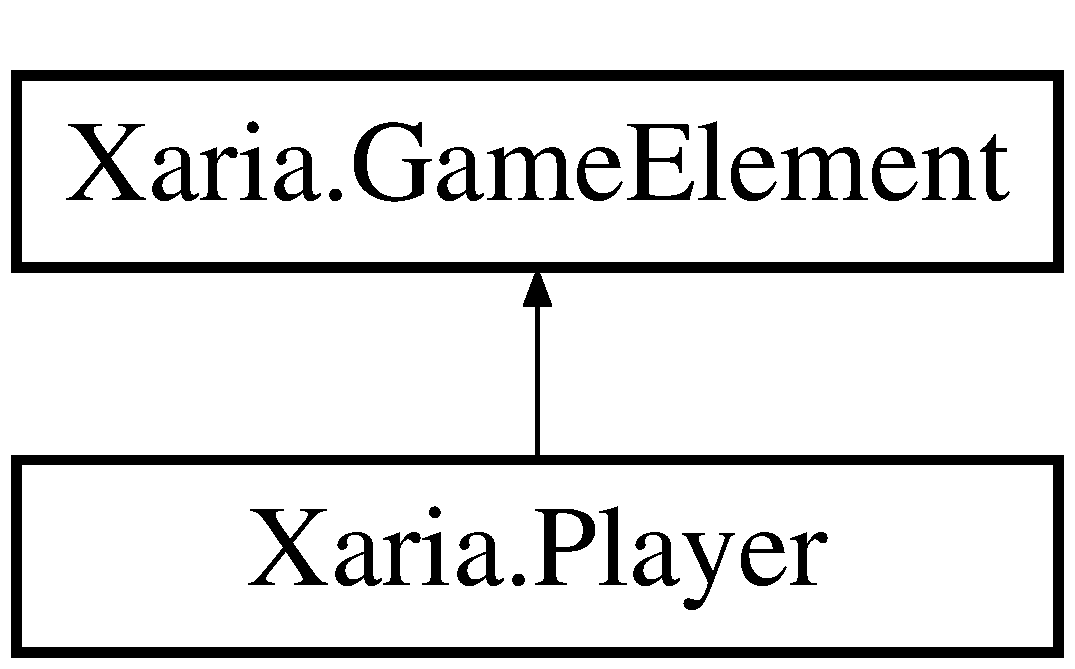
\includegraphics[height=2.000000cm]{classXaria_1_1Player}
\end{center}
\end{figure}
\subsection*{Public Member Functions}
\begin{DoxyCompactItemize}
\item 
\hyperlink{classXaria_1_1Player_a86d80bfee5af015e8612cd992bf53ad0}{Player} ()
\begin{DoxyCompactList}\small\item\em Initializes a new instance of the \hyperlink{classXaria_1_1Player}{Player} class. \end{DoxyCompactList}\item 
override void \hyperlink{classXaria_1_1Player_a25ddea2b9d8679ab6aa649fda6ce1f22}{Draw} (ref Sprite\+Batch sprite\+Batch)
\begin{DoxyCompactList}\small\item\em Draws the player, projectiles, and health. 
\begin{DoxyParams}{Parameters}
{\em sprite\+Batch} & The sprite batch.\\
\hline
\end{DoxyParams}
\end{DoxyCompactList}\item 
bool \hyperlink{classXaria_1_1Player_a75f034f442c2afb88d445ea6968c9a1d}{Is\+Hit} (Projectile shot)
\begin{DoxyCompactList}\small\item\em Determines whether the player is hit by a projectile. \end{DoxyCompactList}\end{DoxyCompactItemize}
\subsection*{Public Attributes}
\begin{DoxyCompactItemize}
\item 
List$<$ Projectile $>$ \hyperlink{classXaria_1_1Player_a643c5dbda599d86c01bde3cfd1749ae6}{Projectiles} = new List$<$Projectile$>$()
\item 
float \hyperlink{classXaria_1_1Player_ae6a69729c15af135388ead356e025b97}{Velocity} = 10
\end{DoxyCompactItemize}
\subsection*{Package Functions}
\begin{DoxyCompactItemize}
\item 
void \hyperlink{classXaria_1_1Player_adc33765b2f4761f7722299cc880f376f}{Update} (Touch\+Collection touch, ref List$<$ List$<$ Enemy $>$$>$ Enemies)
\begin{DoxyCompactList}\small\item\em Updates the specified touch and checks for player projectile collision with enemies. \end{DoxyCompactList}\item 
void \hyperlink{classXaria_1_1Player_a9449bb24ef3a669d4d8081c652811b7c}{Shoot} (Game\+Time game\+Time)
\begin{DoxyCompactList}\small\item\em Shoots a projectile after a given time. \end{DoxyCompactList}\end{DoxyCompactItemize}
\subsection*{Package Attributes}
\begin{DoxyCompactItemize}
\item 
double \hyperlink{classXaria_1_1Player_afdb434cf55e3817ee1f6949c0fb71ee3}{next\+Shoot}
\item 
const int \hyperlink{classXaria_1_1Player_a454099110fca2d19ae08bc7174802018}{S\+T\+A\+R\+T\+I\+N\+G\+\_\+\+H\+E\+A\+L\+TH} = 100
\end{DoxyCompactItemize}
\subsection*{Properties}
\begin{DoxyCompactItemize}
\item 
int \hyperlink{classXaria_1_1Player_a48a4972a17acb525adca1a30454eaf30}{Health}\hspace{0.3cm}{\ttfamily  \mbox{[}get, set\mbox{]}}
\item 
double \hyperlink{classXaria_1_1Player_a0139bb987403bdbe4b795a03be8d2108}{Shoot\+Cooldown}\hspace{0.3cm}{\ttfamily  \mbox{[}get, set\mbox{]}}
\end{DoxyCompactItemize}


\subsection{Detailed Description}
Our player class 



\subsection{Constructor \& Destructor Documentation}
\mbox{\Hypertarget{classXaria_1_1Player_a86d80bfee5af015e8612cd992bf53ad0}\label{classXaria_1_1Player_a86d80bfee5af015e8612cd992bf53ad0}} 
\index{Xaria\+::\+Player@{Xaria\+::\+Player}!Player@{Player}}
\index{Player@{Player}!Xaria\+::\+Player@{Xaria\+::\+Player}}
\subsubsection{\texorpdfstring{Player()}{Player()}}
{\footnotesize\ttfamily Xaria.\+Player.\+Player (\begin{DoxyParamCaption}{ }\end{DoxyParamCaption})\hspace{0.3cm}{\ttfamily [inline]}}



Initializes a new instance of the \hyperlink{classXaria_1_1Player}{Player} class. 



\subsection{Member Function Documentation}
\mbox{\Hypertarget{classXaria_1_1Player_a25ddea2b9d8679ab6aa649fda6ce1f22}\label{classXaria_1_1Player_a25ddea2b9d8679ab6aa649fda6ce1f22}} 
\index{Xaria\+::\+Player@{Xaria\+::\+Player}!Draw@{Draw}}
\index{Draw@{Draw}!Xaria\+::\+Player@{Xaria\+::\+Player}}
\subsubsection{\texorpdfstring{Draw()}{Draw()}}
{\footnotesize\ttfamily override void Xaria.\+Player.\+Draw (\begin{DoxyParamCaption}\item[{ref Sprite\+Batch}]{sprite\+Batch }\end{DoxyParamCaption})\hspace{0.3cm}{\ttfamily [inline]}, {\ttfamily [virtual]}}



Draws the player, projectiles, and health. 
\begin{DoxyParams}{Parameters}
{\em sprite\+Batch} & The sprite batch.\\
\hline
\end{DoxyParams}




Reimplemented from \hyperlink{classXaria_1_1GameElement_a812e0ffbe54519a3fb14a49115bf43d9}{Xaria.\+Game\+Element}.

\mbox{\Hypertarget{classXaria_1_1Player_a75f034f442c2afb88d445ea6968c9a1d}\label{classXaria_1_1Player_a75f034f442c2afb88d445ea6968c9a1d}} 
\index{Xaria\+::\+Player@{Xaria\+::\+Player}!Is\+Hit@{Is\+Hit}}
\index{Is\+Hit@{Is\+Hit}!Xaria\+::\+Player@{Xaria\+::\+Player}}
\subsubsection{\texorpdfstring{Is\+Hit()}{IsHit()}}
{\footnotesize\ttfamily bool Xaria.\+Player.\+Is\+Hit (\begin{DoxyParamCaption}\item[{Projectile}]{shot }\end{DoxyParamCaption})\hspace{0.3cm}{\ttfamily [inline]}}



Determines whether the player is hit by a projectile. 


\begin{DoxyParams}{Parameters}
{\em shot} & The projectile.\\
\hline
\end{DoxyParams}
\begin{DoxyReturn}{Returns}
{\ttfamily true} if the specified player is hit; otherwise, {\ttfamily false}. 
\end{DoxyReturn}
\mbox{\Hypertarget{classXaria_1_1Player_a9449bb24ef3a669d4d8081c652811b7c}\label{classXaria_1_1Player_a9449bb24ef3a669d4d8081c652811b7c}} 
\index{Xaria\+::\+Player@{Xaria\+::\+Player}!Shoot@{Shoot}}
\index{Shoot@{Shoot}!Xaria\+::\+Player@{Xaria\+::\+Player}}
\subsubsection{\texorpdfstring{Shoot()}{Shoot()}}
{\footnotesize\ttfamily void Xaria.\+Player.\+Shoot (\begin{DoxyParamCaption}\item[{Game\+Time}]{game\+Time }\end{DoxyParamCaption})\hspace{0.3cm}{\ttfamily [inline]}, {\ttfamily [package]}}



Shoots a projectile after a given time. 


\begin{DoxyParams}{Parameters}
{\em game\+Time} & The game time.\\
\hline
\end{DoxyParams}
\mbox{\Hypertarget{classXaria_1_1Player_adc33765b2f4761f7722299cc880f376f}\label{classXaria_1_1Player_adc33765b2f4761f7722299cc880f376f}} 
\index{Xaria\+::\+Player@{Xaria\+::\+Player}!Update@{Update}}
\index{Update@{Update}!Xaria\+::\+Player@{Xaria\+::\+Player}}
\subsubsection{\texorpdfstring{Update()}{Update()}}
{\footnotesize\ttfamily void Xaria.\+Player.\+Update (\begin{DoxyParamCaption}\item[{Touch\+Collection}]{touch,  }\item[{ref List$<$ List$<$ Enemy $>$$>$}]{Enemies }\end{DoxyParamCaption})\hspace{0.3cm}{\ttfamily [inline]}, {\ttfamily [package]}}



Updates the specified touch and checks for player projectile collision with enemies. 


\begin{DoxyParams}{Parameters}
{\em touch} & The touch.\\
\hline
{\em Enemies} & The enemies.\\
\hline
\end{DoxyParams}


\subsection{Member Data Documentation}
\mbox{\Hypertarget{classXaria_1_1Player_afdb434cf55e3817ee1f6949c0fb71ee3}\label{classXaria_1_1Player_afdb434cf55e3817ee1f6949c0fb71ee3}} 
\index{Xaria\+::\+Player@{Xaria\+::\+Player}!next\+Shoot@{next\+Shoot}}
\index{next\+Shoot@{next\+Shoot}!Xaria\+::\+Player@{Xaria\+::\+Player}}
\subsubsection{\texorpdfstring{next\+Shoot}{nextShoot}}
{\footnotesize\ttfamily double Xaria.\+Player.\+next\+Shoot\hspace{0.3cm}{\ttfamily [package]}}

\mbox{\Hypertarget{classXaria_1_1Player_a643c5dbda599d86c01bde3cfd1749ae6}\label{classXaria_1_1Player_a643c5dbda599d86c01bde3cfd1749ae6}} 
\index{Xaria\+::\+Player@{Xaria\+::\+Player}!Projectiles@{Projectiles}}
\index{Projectiles@{Projectiles}!Xaria\+::\+Player@{Xaria\+::\+Player}}
\subsubsection{\texorpdfstring{Projectiles}{Projectiles}}
{\footnotesize\ttfamily List$<$Projectile$>$ Xaria.\+Player.\+Projectiles = new List$<$Projectile$>$()}

\mbox{\Hypertarget{classXaria_1_1Player_a454099110fca2d19ae08bc7174802018}\label{classXaria_1_1Player_a454099110fca2d19ae08bc7174802018}} 
\index{Xaria\+::\+Player@{Xaria\+::\+Player}!S\+T\+A\+R\+T\+I\+N\+G\+\_\+\+H\+E\+A\+L\+TH@{S\+T\+A\+R\+T\+I\+N\+G\+\_\+\+H\+E\+A\+L\+TH}}
\index{S\+T\+A\+R\+T\+I\+N\+G\+\_\+\+H\+E\+A\+L\+TH@{S\+T\+A\+R\+T\+I\+N\+G\+\_\+\+H\+E\+A\+L\+TH}!Xaria\+::\+Player@{Xaria\+::\+Player}}
\subsubsection{\texorpdfstring{S\+T\+A\+R\+T\+I\+N\+G\+\_\+\+H\+E\+A\+L\+TH}{STARTING\_HEALTH}}
{\footnotesize\ttfamily const int Xaria.\+Player.\+S\+T\+A\+R\+T\+I\+N\+G\+\_\+\+H\+E\+A\+L\+TH = 100\hspace{0.3cm}{\ttfamily [package]}}

\mbox{\Hypertarget{classXaria_1_1Player_ae6a69729c15af135388ead356e025b97}\label{classXaria_1_1Player_ae6a69729c15af135388ead356e025b97}} 
\index{Xaria\+::\+Player@{Xaria\+::\+Player}!Velocity@{Velocity}}
\index{Velocity@{Velocity}!Xaria\+::\+Player@{Xaria\+::\+Player}}
\subsubsection{\texorpdfstring{Velocity}{Velocity}}
{\footnotesize\ttfamily float Xaria.\+Player.\+Velocity = 10}



\subsection{Property Documentation}
\mbox{\Hypertarget{classXaria_1_1Player_a48a4972a17acb525adca1a30454eaf30}\label{classXaria_1_1Player_a48a4972a17acb525adca1a30454eaf30}} 
\index{Xaria\+::\+Player@{Xaria\+::\+Player}!Health@{Health}}
\index{Health@{Health}!Xaria\+::\+Player@{Xaria\+::\+Player}}
\subsubsection{\texorpdfstring{Health}{Health}}
{\footnotesize\ttfamily int Xaria.\+Player.\+Health\hspace{0.3cm}{\ttfamily [get]}, {\ttfamily [set]}}

\mbox{\Hypertarget{classXaria_1_1Player_a0139bb987403bdbe4b795a03be8d2108}\label{classXaria_1_1Player_a0139bb987403bdbe4b795a03be8d2108}} 
\index{Xaria\+::\+Player@{Xaria\+::\+Player}!Shoot\+Cooldown@{Shoot\+Cooldown}}
\index{Shoot\+Cooldown@{Shoot\+Cooldown}!Xaria\+::\+Player@{Xaria\+::\+Player}}
\subsubsection{\texorpdfstring{Shoot\+Cooldown}{ShootCooldown}}
{\footnotesize\ttfamily double Xaria.\+Player.\+Shoot\+Cooldown\hspace{0.3cm}{\ttfamily [get]}, {\ttfamily [set]}}



The documentation for this class was generated from the following file\+:\begin{DoxyCompactItemize}
\item 
Project3/\+Project3/\hyperlink{Player_8cs}{Player.\+cs}\end{DoxyCompactItemize}

\chapter{File Documentation}
\hypertarget{Activity1_8cs}{}\section{Project3/\+Project3/\+Activity1.cs File Reference}
\label{Activity1_8cs}\index{Project3/\+Project3/\+Activity1.\+cs@{Project3/\+Project3/\+Activity1.\+cs}}
\subsection*{Classes}
\begin{DoxyCompactItemize}
\item 
class \hyperlink{classXaria_1_1Activity1}{Xaria.\+Activity1}
\begin{DoxyCompactList}\small\item\em The android activity \end{DoxyCompactList}\end{DoxyCompactItemize}
\subsection*{Namespaces}
\begin{DoxyCompactItemize}
\item 
namespace \hyperlink{namespaceXaria}{Xaria}
\end{DoxyCompactItemize}

\hypertarget{Button_8cs}{}\section{Project3/\+Project3/\+Button.cs File Reference}
\label{Button_8cs}\index{Project3/\+Project3/\+Button.\+cs@{Project3/\+Project3/\+Button.\+cs}}
\subsection*{Classes}
\begin{DoxyCompactItemize}
\item 
class \hyperlink{classXaria_1_1Button}{Xaria.\+Button}
\begin{DoxyCompactList}\small\item\em The button class \end{DoxyCompactList}\end{DoxyCompactItemize}
\subsection*{Namespaces}
\begin{DoxyCompactItemize}
\item 
namespace \hyperlink{namespaceXaria}{Xaria}
\end{DoxyCompactItemize}

\hypertarget{Game1_8cs}{}\section{Project3/\+Project3/\+Game1.cs File Reference}
\label{Game1_8cs}\index{Project3/\+Project3/\+Game1.\+cs@{Project3/\+Project3/\+Game1.\+cs}}
\subsection*{Classes}
\begin{DoxyCompactItemize}
\item 
class \hyperlink{classXaria_1_1Game1}{Xaria.\+Game1}
\begin{DoxyCompactList}\small\item\em This is the main type for your game. \end{DoxyCompactList}\end{DoxyCompactItemize}
\subsection*{Namespaces}
\begin{DoxyCompactItemize}
\item 
namespace \hyperlink{namespaceXaria}{Xaria}
\end{DoxyCompactItemize}
\subsection*{Enumerations}
\begin{DoxyCompactItemize}
\item 
enum \hyperlink{namespaceXaria_a2c2420c982c39ab01bdb72f1d7d4aac7}{Xaria.\+Game\+State} \{ \hyperlink{namespaceXaria_a2c2420c982c39ab01bdb72f1d7d4aac7aa6122a65eaa676f700ae68d393054a37}{Xaria.\+Game\+State.\+Start}, 
\hyperlink{namespaceXaria_a2c2420c982c39ab01bdb72f1d7d4aac7ac9dbb2b7c84159b632d71e512eba8428}{Xaria.\+Game\+State.\+Playing}, 
\hyperlink{namespaceXaria_a2c2420c982c39ab01bdb72f1d7d4aac7a87557f11575c0ad78e4e28abedc13b6e}{Xaria.\+Game\+State.\+End}
 \}\begin{DoxyCompactList}\small\item\em Game\+State controls the game\textquotesingle{}s state \end{DoxyCompactList}
\end{DoxyCompactItemize}

\hypertarget{GameElement_8cs}{}\section{Project3/\+Project3/\+Game\+Element.cs File Reference}
\label{GameElement_8cs}\index{Project3/\+Project3/\+Game\+Element.\+cs@{Project3/\+Project3/\+Game\+Element.\+cs}}
\subsection*{Classes}
\begin{DoxyCompactItemize}
\item 
class \hyperlink{classXaria_1_1GameElement}{Xaria.\+Game\+Element}
\begin{DoxyCompactList}\small\item\em Basic element that stores texture, position, and draw info. \end{DoxyCompactList}\end{DoxyCompactItemize}
\subsection*{Namespaces}
\begin{DoxyCompactItemize}
\item 
namespace \hyperlink{namespaceXaria}{Xaria}
\end{DoxyCompactItemize}

\hypertarget{Level_8cs}{}\section{Project3/\+Project3/\+Level.cs File Reference}
\label{Level_8cs}\index{Project3/\+Project3/\+Level.\+cs@{Project3/\+Project3/\+Level.\+cs}}
\subsection*{Classes}
\begin{DoxyCompactItemize}
\item 
class \hyperlink{classXaria_1_1Level}{Xaria.\+Level}
\begin{DoxyCompactList}\small\item\em The \hyperlink{classXaria_1_1Level}{Level} class \end{DoxyCompactList}\end{DoxyCompactItemize}
\subsection*{Namespaces}
\begin{DoxyCompactItemize}
\item 
namespace \hyperlink{namespaceXaria}{Xaria}
\end{DoxyCompactItemize}

\hypertarget{Player_8cs}{}\section{Project3/\+Project3/\+Player.cs File Reference}
\label{Player_8cs}\index{Project3/\+Project3/\+Player.\+cs@{Project3/\+Project3/\+Player.\+cs}}
\subsection*{Classes}
\begin{DoxyCompactItemize}
\item 
class \hyperlink{classXaria_1_1Player}{Xaria.\+Player}
\begin{DoxyCompactList}\small\item\em Our player class \end{DoxyCompactList}\end{DoxyCompactItemize}
\subsection*{Namespaces}
\begin{DoxyCompactItemize}
\item 
namespace \hyperlink{namespaceXaria}{Xaria}
\end{DoxyCompactItemize}

%--- End generated contents ---

% Index
\backmatter
\newpage
\phantomsection
\clearemptydoublepage
\addcontentsline{toc}{chapter}{Index}
\printindex

\end{document}
